% !TeX root = thesis.tex
% !TeX spellcheck = en_GB
% !TeX encoding = UTF-8


\documentclass[12pt,a4paper,oneside]{amsbook}

\usepackage{thesis}


\begin{document}


\frontmatter

% Half-title

% Title page
% !TeX root = thesis.tex
% !TeX spellcheck = en_GB
% !TeX encoding = UTF-8


\begin{titlepage}
	\begin{center}

		% Logos
		
\includegraphics[width=\textwidth]{logos.jpg} \\[3em]

		% Programme information
		{\Large\bfseries Erasmus Mundus Consortium} \\[1em]
		{\LARGE\bfseries MathMods} \\[2em]
		
		% Joint degree
		{\large Joint Degree of Master of Science in} \\
		{\large Mathematical Modelling in Engineering: Theory, Numerics, Applications} \\[1em]
		
		{\large In the framework of the} \\
		{\large Consortium Agreement and Award of a Joint/Multiple Degree 2013-2019} \\[3em]
		
		% Title
		{\LARGE Master's Thesis} \\[2em]
%		\hrule
		{\Huge\bfseries The Singular Points method for pricing exotic path-dependent options}
%		\hrule \leavevmode
		\\[4em]

		% Supervisor
		\begin{minipage}[t]{0.5\textwidth}
			\begin{center} \Large
				\emph{Supervisor:} \\
				\textsc{\LARGE Prof. \textbf{Fabio Antonelli}}
			\end{center}
		\end{minipage}
		\begin{minipage}[t]{0.4\textwidth}
			\begin{center} \Large
				\emph{Candidate:}\\
				{\LARGE\textbf{\textsc{Sudip Sinha}}}\\
				Matricola: 228435
			\end{center}
		\end{minipage}
		
		\vfill

		% Bottom of the page
		{\large \today}

	\end{center}
\end{titlepage}


%%% Local Variables:
%%% mode: latex
%%% TeX-master: t
%%% End:


%Research is what I’m doing when I don’t know what I’m doing. — Wernher von Braun

% Information (copyright notice, ISBN, etc.)

% Dedication if any, else empty

\tableofcontents

%\clearpage


% Preface chapter
\chapter*{Preface}
\label{cha:preface}
% !TeX root = ../thesis.tex
% !TeX spellcheck = en_GB
% !TeX encoding = UTF-8

A path-dependent option is a type of exotic option in which the price of the option depends not only on the price of the underlying asset at maturity, but also on the history of the asset's price till that point. Typical examples of popular exotic options are Asian options, lookback options, barrier options, and digital options.

In the Black-Scholes market model, it is not possible to find closed-form analytical formulae for the prices of most exotic options. This inspires the requirement of fast numerical algorithms to determine the fair price of such options. Such algorithms may be clustered into categories. Some algorithms utilise the convergence of prices calculated using a discrete model to those of a continuous model, as a limit when the time step is reduced. Other approaches include use of numerical methods to solve partial differential equation, or simulation using Monte Carlo methods.

Under the Cox-Ross-Rubinstein model, Gaudenzi\footnote{\url{http://people.uniud.it/page/marcellino.gaudenzi}}, Zanette\footnote{\url{http://people.uniud.it/page/antonino.zanette}} and Lepellere\footnote{\url{https://www.researchgate.net/profile/Maria_Lepellere}} introduced the Singular Points method. It is a numerical method to price Asian and lookback options. A modification enables pricing of cliquet options. In the method, in each node of the binomial tree of the underlying risky asset, the price is represented as a continuous function of the path-dependent parameter. An advantage of this method over pre-existing methods is its low order of computational and space complexity. It is convergent, and allows us to set \emph{a priori} upper and lower bounds on the error.

In the master's thesis, we present an exposition on the Singular Points method and how it may be used to price exotic options. We also explore the extensibility of the method to similar types of options, like Asian options with geometric mean as opposed to arithmetic mean, and whether it may be used for variable local volatilities and interest rates.


\paragraph{Prerequisites}
The reader is expected to be familiar about basic Probability Theory and Stochastic Processes. In particular, (s)he should be comfortable with probability spaces and measures, filtrations, random variables, stochastic processes, martingales, Brownian motion, and elementary stochastic calculus. There is no strict requirement of knowledge of financial concepts, as we introduce the required terminologies in the introductory chapters. [TODO: Appendix]


\paragraph{Note to the reader}
The theory part of the thesis borrows heavily from the book titled Introduction to Stochastic Calculus Applied to Finance by Damien Lamberton and Bernard Lapeyre \cite[]{Lamberton1996}, as well as from the lecture notes of Mathematical Finance authored by Prof. Fabio Antonelli. This course was offered in the Fall semester of 2014-15 in Università degli Studi dell'Aquila, Italy.

The chapters on the Singular Point method has been motivated by the series of papers published by Gaudenzi, Zanette and Lepellere on the same topic.


%%% Local Variables:
%%% mode: latex
%%% TeX-master: t
%%% End:



\chapter*{Notations}
\begin{description}
	\item[$ {[n]} $] $ \{0, 1, 2, \dots, n\} $
	\item[$ \mathbb{N} $] $ \{ 1, 2, 3, \dots \} $
	\item[$ \mathbb{N}_0 $] $ \mathbb{N} \cup \{ 0 \} $
	\item[$ \mu \mathcal{F} $] The class of all $ \mathcal{F} $-measurable functions.
	\item[$ \floor{\cdot} $] The floor function. $ \floor{x} $ gives the largest integer smaller or equal to $ x $.
	\item[$ \ceil{\cdot} $] The ceiling function. $ \ceil{x} $ gives the smallest integer larger or equal to $ x $.
	\item[$ \sim $] Represents the discounted value when used on top of a quantity. For example, $ \tilde{S}_t = e^{-rt} S_t $
\end{description}


\mainmatter

\chapter{Prologue}
\label{cha:prologue}
% !TeX root = ../thesis.tex
% !TeX spellcheck = en_GB
% !TeX encoding = UTF-8


Mathematics and finance have been intricately linked since the inception of human civilisations. In the span of the last two millennia, many mathematicians -- from Thales of Greece to Fibonacci, Pascal, Fermat and Bernoulli -- have tried to apply their knowledge to the domain of finance\footnote{Significant portions in this introductory section have been taken verbatim from the paper \cite{Akyildirim2014}}. However, Louis Bachelier's thesis “Théorie de la Spéculation” (Theory of Speculation) in 1900 arguably marked the birth of modern mathematical finance. Bachelier is credited with being the first person to derive the mathematics of Brownian motion and to apply its trajectories for modelling stock price dynamics and calculating option prices.

One of the most exciting innovations in the modern history of mathematical finance is rooted in the discovery of the Brownian motion by Scottish botanist Robert Brown. In 1827, he observed rapid oscillatory motion of microscopic particles in a fluid resulting from their collision with atoms or molecules in the fluid. However, Bachelier was the first to define Brownian motion mathematically, and used the one dimensional version $ t \mapsto B_t, t \ge 0 $ to model stock price dynamics. Norbert Wiener laid down the rigorous mathematical foundation of Browian motion, hence the parallel name of Wiener process is also used for Brownian motion. He proved the existence of Brownian motion, and constructed the Wiener measure which describes its probability distribution.

In 1933, in the seminal book “Foundations of the Theory of Probability”, Kolmogorov laid the foundation of modern Probability theory from fundamental axioms. His work relied heavily on Lebesgue's Measure Theory, and united the previously disparate areas of probability -- discrete and continuous -- into a unified theory that could be applied to both. It is in this book that he introduced the ideas of conditional expectation and equivalent measures.

Another breakthrough in Probability theory came in 1941, when in his attempts to model Markov processes, Kiyosi Itô (in his famous 1942 paper “On stochastic processes”) constructed stochastic differential equations of the form $ \dif X_t = \mu(X_t) \dif t + \sigma(X_t) \dif B_t $, where $ B_t $ is a standard Brownian motion. He introduced the theory of integration over a Brownian motion, and in 1951 gave a formula for constructing new stochastic differntial equations from existing ones (Itô's lemma), giving birth to Itô calculus. Itô's lemma is one of the most widely used mathematical formula by financial engineers today.

At this crucial juncture, when the probability theory was ripe enough, in 1973, Fischer Black and Myron Scholes published the paper “The Pricing of Options and Corporate Liabilities”, and Robert Merton published the paper “On the pricing of corporate debt: the risk structure of interest rates”. These papers together introduced a new methodology for the valuation of financial instruments and in particular developed the Black–Scholes model for pricing European call and put options. At the same time, another breakthrough on the industry side was the foundation of the Chicago Board Options Exchange to become the first marketplace for trading listed options. Even beyond the imagination of the celebrated authors above, the market was so quick to adapt these models. By 1975, almost all traders were valuing and hedging option portfolios by using the Black–Scholes model built in their hand calculators.

But there were problems with the Black and Scholes model. A primary disadvantage was that the esoteric theory was not understandable by most practitioners in the field of finance. Moreover, it could not be used to price all kinds of options. In 1979, Cox, Ross and Rubinstein introduced a discrete model, which is much more approachable, and yet has the flexibility to price almost all kinds of derivatives. Yet, the exponential nature of the complexity forbids scaling up the number of levels of the tree to any significant value, reducing its utility.

In this chapter, we briefly discuss some fundamental ideas in finance. We shall follow this up with a discussion on the two models mentioned.


\section{Financial instruments}
\label{sec:intro-assets}

A \emph{financial instrument} or a \emph{financial asset} is an intangible asset whose value is derived from a contractual claim, such as bank deposits, bonds, stocks and derivatives. Financial assets are usually more \emph{liquid} than other tangible assets, such as commodities or real estate, and may be traded on financial markets. Every financial asset is characterised by its return. When the return is deterministic, we call it a \emph{risk-free} or \emph{riskless} asset. When the return is contingent on the market and external conditions, it is called \emph{risky}. It must be kept in mind that no instrument is fundamentally risk-free, it has only negligible risk compared to its risky counterparts.



\subsection{Return on an asset}
\label{subsec:intro-assets-return}

\paragraph{Return on a riskless asset -- Compounding}
Compounding is the first idea that we must be familiar with. Essentially, a riskless asset will increase in monetary value in a deterministic manner if we keep it in the market. The increase depends on the compounding frequency and the duration of investment. The term compounding is used because the interest earned in each period also contributes to the principal in the successive periods.

Let the compounding frequency is $ n $ times per year, the total time is $ t $, and the annual rate of interest is $ r $. Then
\begin{equation}
	\label{eq:intro-compounding-discrete}
	B_t = B_0 \left(1 + \frac{r}{n} \right)^{\floor{nt}},
\end{equation}
where $ B_0 $ is the starting value of the asset, and $ B_t $ is the value of the asset at time $ t $, and $ \floor{\cdot} $ represents the floor function.

If the compounding is continuous, we let $ n \to \infty $ to obtain
\begin{equation}
	\label{eq:intro-compounding-continous}
	B_t = B_0 e^{rt}.
\end{equation}


\paragraph{Return on a risky asset}
At any point of time in the future, the value of a risky asset is not known with certainty, so it is a random variable taking values in $ [0, \infty) $. Since the values change with time, we denote the \emph{spot price} of a risky asset by the stochastic process\footnote{\url{https://en.wikipedia.org/wiki/Stochastic_process}} $ (S_t)_t $, where $ t \in [0, T] $ denotes the time and $ T $ is the maturity. Since the future value of the asset is adventitious, we use the following quantities to measure the return of the risky asset in the given time interval.

\begin{dfn}[absolute and relative returns]
	The absolute return on an asset for the time interval $ [0, t], \  t \in [0, T] $ is given by
	\begin{equation*}
		\tilde{R}_t = S_t - S_0
	\end{equation*}
	
	The relative return on the asset is given by
	\begin{equation*}
		R_t = \frac{S_t - S_0}{S_0}
	\end{equation*}	
\end{dfn}

It must be noted that relative return is usually a better indicator of the return on an asset as compared to its absolute equivalent. This may be illustrated better by the following example.
\begin{eg}[relative vs absolute return]
	Let A and B be two assets. Let their values at $ t = 0 $ be $ S_0^A = 5 $ and $ S_0^B = 10 $, respectively. At time $ t = 1 $ one observes that the prices have become $ S_1^A = 10 $ and $ S_1^B = 15 $.
	
	The absolute return on both assets are equal to $ 5 $ here. On the other hand, the relative returns are:
	\begin{align*}
		R_1^A  &=  \frac{S_1^A - S_0^A}{S_0^A} = \frac{5}{5} = 1  \\
		R_1^B  &=  \frac{S_1^B - S_0^B}{S_0^B} = \frac{5}{10} = \frac{1}{2}
	\end{align*}
	
	Thus, the asset A is more interesting to an investor, as it gives more return on investment. If an investor were to invest an amount of $ 10 $ at $ t = 0 $, it is more profitable for him to buy two quantities of asset A than one quantity of asset B.
\end{eg}


\subsection{Common asset types}

\paragraph{Bonds}
A \emph{bond} is an instrument of indebtedness of the bond issuer to the holders. It is a \emph{debt security}, under which the issuer owes the holders a debt and, depending on the terms of the bond, is obliged to pay them interest (the coupon) and/or to repay the principal at a later date, termed the maturity date. Bonds can also be thought of as a \emph{loan} given to the issuer of the bond by the holder. A bond primarily has two kinds of risks, \emph{credit default risk} and \emph{interest rate risk}. A bond issued by a reliable institution like the United States government is a good illustration of a risk-free asset. This is because the probability of such an organisation defaulting is close to zero, or in other words, the bond has \emph{negligible} \emph{credit default risk}. Such bonds are only subject to fluctuations of the current interest rate, called \emph{interest rate risk}. The interest rate risk may also be nullified if the bond is held till maturity. If we assume that the interest rate is deterministic (the fluctuations are not random), the value of the bond is computable at any given future date, making it riskless. Such an assumption is quite reasonable in short periods of time and for institutions with a low default risk rating.


\paragraph{Stocks}
A \emph{stock} of a corporation is an ownership certificate, and constitutes the equity stake of its owners. It represents the residual assets of the company that would be due to stockholders after discharge of all senior claims such as secured and unsecured debt. A \emph{share} of a stock is a unit of ownership of the organisation. Stocks are inherently risky, since the value of the organisation may change from time to time due to various internal and external factors. As noted earlier, since stocks are risky, the value of a stock in time is represented by a stochastic process $ (S_t)_t $.


\paragraph{Derivatives}
A \emph{derivative} is a contract between two parties that specify conditions (starting and termination dates, resulting values and definitions of the underlying variables, the parties' contractual obligations, and the notional amount) under which transactions are to be made between the parties. The most common underlying assets include commodities, stocks, bonds, interest rates and currencies, but they can also be other derivatives, which adds another layer of complexity to proper valuation. Essentially, the value of a derivative is a function of the value of the \emph{underlying} asset(s). Derivatives are traded in their own right, and a fair price must be found for a derivative at each time of its existence. This problem is known as the \emph{pricing problem}. One of the primary motivations for creation of derivatives was to hedge one's position from fluctuations in the market. A \emph{hedge} is an investment strategy intended to offset potential losses or gains that may be incurred by a companion investment. Finding a hedging strategy is called the \emph{hedging problem}. These are the two problems that must be looked at when defining a market model. In this thesis, our main focus shall be the pricing problem of a particular class of derivatives, called \emph{exotic options}.


\subsection{Classification of derivatives}
\label{subsec:intro-derivative-classification}

Derivatives may be classified on the basis of various factors. One important factor is whether the risk is shared, or taken up by only one party. Another factor is the nature of the function (of the underlying) that the derivative depends on. This function may either be dependent only on the final value of the underlying (\emph{path-independent}), or on the path that it took to reach this final value (\emph{path-dependent}). The function may be discrete (\emph{digital} or \emph{binary}), or continuous In this section, we briefly look at some of the more important types of derivatives. \footnote{
	A more interested reader should consult the following extensive Wikipedia articles.
	\begin{itemize}
		\item \url{https://en.wikipedia.org/wiki/Option_(finance)\#Types}
		\item \url{https://en.wikipedia.org/wiki/Option_style}
	\end{itemize}
}


\paragraph{Futures and forwards}

\begin{dfn}[Futures and forwards]
	Futures and forwards are contracts between two parties, the seller and the buyer, to exchange a certain asset at a predetermined future time at a agreed upon price. Futures are \emph{exchange-traded derivatives} (ETDs), whereas forwards are traded \emph{over-the-counter} (OTC).
\end{dfn}

Such derivatives obligate the contractual parties to the terms over the life of the contract. Futures are in some sense `safer' compared to forwards, since the involved parties must go through standard protocols of the exchange.
The contract contains the following details.
\begin{description}
	\item[$ T $] The maturity, or the duration of the contract
	\item[$ F_0 $] The delivery price, or the price prefixed (at the initial time) at which trades must take place at maturity
	\item[$ r $] The rate of interest
	\item[underlying] The asset(s) of trade at maturity
	\item[$ S_0 $] The initial value of the underlying asset(s)
\end{description}
There are, of course, other possibilities, for instance a variable interest rate, dividends yielded by the underlying, but these may be viewed as generalisations of this simple case.

Let us assume that the compounding is continuous. We may show that under the condition of a \emph{viable market}\footnote{see Section \ref{sec:intro-market} for definitions of the term}, the fair delivery price of a future with underlying prices $ ( S_t )_{t \in [0, T] } $ at any time $ t \in [0, T] $ is given by the following equation.
\begin{equation}
	\label{eq:intro-future-pr}
	F_t = S_t e^{ r (T - t) }
\end{equation}


\paragraph{Options}

\begin{dfn}[option]
	An \emph{option} or a \emph{contingent claim} is a derivative which provides the buyer \emph{the right, but not the obligation} to enter the contract under the specified terms.
\end{dfn}

Thus, the owner of the option may choose whether to exercise his right or not. Thus, on the one hand, the owner of the option bears no risk, since all the choice is his. On the other hand, the seller of the option is \emph{obligated} to honour the terms of the contract -- whether it benefits him or not -- essentially making him bear all the risks. This asymmetry is primarily what sets options apart from the futures and forwards discussed earlier.
The contract contains the following details.
\begin{description}
	\item[$ T $] The maturity, or the duration of the contract
	\item[$ K $] The strike price, or the prefixed price at which trades may take place at maturity
	\item[$ r $] The rate of interest
	\item[underlying] The asset(s) which may be traded at maturity
	\item[$ S_0 $] The initial value of the underlying asset at the initial time
	\item[right] The exact right that the owner of the options has (see below)
	\item[exercise time] European or American (see below)
\end{description}

Options may be categorised by the right of the owner and the exercise time.

\subparagraph{According to the right of the owner}  Options may be of two main types.
\begin{description}
	\item[call] The owner has the right to buy. In this case, the price of the option at maturity is given by $ c_T = (S_T - K)_+ $, where $ (x)_+ \coloneqq \max \{ 0, x \} $.
	\item[put] The owner has the right to sell. In this case, the price of the option at maturity is given by $ p_T = (K - S_T)_+ $.
\end{description}
Of course, other complicated ownership rights may be constructed, but we shall not go into the details of those.

\subparagraph{According to the time at which the option may be exercised}  Again, option may be of two main types.
\begin{description}
	\item[European] The owner may exercise the option only at maturity
	\item[American] The owner may exercise the option at any time up to the maturity
\end{description}
Again, more complicated options exist, which allow exercising rights only at certain time points, but we exclude them from out discussion.

Since American options allow for more flexibility for the owner, and thus more risk for the seller, they are more expensive as compared to their European counterparts. Let $ c_t, p_t $ denote the prices of an European call and put, and $ C_t, P_t $ denote the prices of an American call and put, respectively. Then, we must have $ C_t \ge c_t $ and $ P_t \ge p_t $.


\subparagraph{Call-put parity}  Call and put prices are connected to each other. We need the following proposition to explore the relationship.

\begin{prp}[Equality of portfolios]
	\label{thm:intro-portfolio-eq}
	In a \emph{viable} and \emph{frictionless market}\footnote{see Section \ref{sec:intro-market} for definitions of the terms}, if the values of two portfolios coincide at a time $ T $, they have to coincide at $ 0 $ ( or any other intermediate time $ t $).
\end{prp}

\begin{proof}
	Let us denote by $ \mathcal{P}_1 $ and $ \mathcal{P}_2 $ the two portfolios and by $ v_t(\mathcal{P}) $ the value of a portfolio $ \mathcal{P} $ at time $ t $. By assumption $ v_T (\mathcal{P}_1) = v_T (\mathcal{P}_2) $, so we assume by contradiction that $ v_0 (\mathcal{P}_1) > v_0 (\mathcal{P}_2) $.
	
	Under this hypothesis it is possible to construct the following arbitrage strategy. At time 0, one can borrow the portfolio $ \mathcal{P}_1 $ and sell it right away to buy portfolio $ \mathcal{P}_2 $. One can pocket the difference $ v_0 (\mathcal{P}_1) - v_0 (\mathcal{P}_2) > 0 $. At $ t = T $ the values of the two portfolios coincide, so selling $ \mathcal{P}_2 $ one gets the exact money to buy $ \mathcal{P}_1 $ to be returned to the original lender. An profit is achieved, without investing any money, implying an arbitrage and violating the viable market hypothesis.
	
	Similarly, we can show that $ v_0 (\mathcal{P}_1) < v_0 (\mathcal{P}_2) $ would also enable an arbitrage opportunity. Generalising the argument to all intermediate times $ t \in [0, T] $, we get the result.
\end{proof}

We now look at the relationship. $ S_T - K = (S_T - K)_+ + (S_T - K)_- = (S_T - K)_+ - (K - S_T)_+ = c_T - p_T $. For any general time $ t $, using Proposition \ref{thm:intro-portfolio-eq}, it holds that $ c_t - p_t = S_t - K e^{- r (T-t) } $. This is known as the \emph{call-put parity}.


\paragraph{Exotic options}
European options are path-independent and the simplest type of options available. Hence, they are popularly known as \emph{vanilla options}. The American options are path-dependent. Typically, other options which are more complex in nature are collectively called \emph{exotic options}. These are usually path-dependent, and may be either European, American or have more complex exercise times. A few such options are described in brief.
\begin{description}
	\item[Asian] The payoff depends on the average of the underlying's prices
	\item[lookback] The payoff depends on one of the extrema of the underlying's prices
	\item[cliquet or ratchet] A series of globally or locally, capped or floored, at-the-money options, but where the total premium is determined in advance.
	\item[barrier] The price of the underlying reaching the pre-set barrier level either springs the option into existence (\emph{knock-in}) or extinguishes an already existing option (\emph{knock-out}).
\end{description}



\section{Financial Markets}
\label{sec:intro-market}

The idea of financial markets is intricately linked to that of financial transactions. Analogous to the ordinary markets, a financial market is a human construct to allow transaction between investors. The assets in the financial market are typically financial instruments such as bonds, stocks and derivatives discussed in the previous section. In this section we will primarily concern ourselves with the nature of financial markets and the assumptions we make while modelling them. Some of the jargon used in the previous section will become clear after this section.

Pricing of financial assets is one of the most pressing aims of the subject of Financial Mathematics. In order to do so, we need to understand and characterise the fundamental mechanisms of the market that shape the pricing of assets. In doing so, we must note which dynamics of the market are most fundamental and must be incorporated in every model, and which are more debatable may be excluded from simpler models.

\paragraph{Viable market}
The term viability here refers to the fairness of a market. To interpret viability, we need to familiarise ourselves with the following definitions.

In what follows, we assume the following.
\begin{itemize}
	\item There is a probability space $ (\Omega, \mathcal{F}, (\mathcal{F}_t)_t, P) $, endowed with the filtration $ (\mathcal{F}_t)_t $.
	\item $ \forall t \in [0, T], T \in [0, \infty) $, there is one riskless asset worth $ S_t^0 = e^{rt} $ (Take $ S_0^0 = 1 $).
	\item $ \forall t \in [0, T], T \in [0, \infty) $, there are $ d $ risky assets each worth $ S_t^i $, where $ i \in \{ 1, 2, \dots, d \} $ is the index of the risky asset. These may be represented as a $ d $-dimensional (vector) stochastic process $ ( S_t^1, S_t^2, \dots, S_t^d ) $.
\end{itemize}

Also, any quantity with a `$ \sim $' on top denotes the discounted value of that quantity.


\begin{dfn}[investment strategy]
	A $ d + 1 $ dimensional (vector) stochastic process $ \Phi = (\bm{\phi_t})_t = (\phi_t^0, \phi_t^1, \dots, \phi_t^d)_t $ is called an \emph{investment strategy} or \emph{trading strategy} if $ \phi_t^i $ is $ \mathcal{F}_t $-measurable $ \forall i \in [d] $.
\end{dfn}
This means that there is a procedure to allocate resources within the portfolio at all times. We shall write strategy to mean investment strategy in the rest of the document.

The following definition gives the value of a strategy at a point in time.
\begin{dfn}[value of a strategy]
	The value of a strategy $ \Phi $ at a time $ t $ is given by $ V_t( \Phi ) = \bm{\phi_t} \cdot S_t $.
\end{dfn}

\begin{dfn}[self-financing strategy]
	A portfolio is self-financing if its changes in value are only due to changes in prices of the assets. This can be represented as follows.
	\begin{subequations}
		\begin{align}
			\dif V_t &= \bm{\phi_t} \cdot \dif S_t \qquad \forall t \in [0, T]  \\
			\implies  \qquad  \dif \tilde{V}_t &= \bm{\phi_t} \cdot \dif \tilde{S}_t \qquad \forall t \in [0, T]
		\end{align}
	\end{subequations}
\end{dfn}
This implies that we do not put in any fresh money in the strategy at any point of time, apart from what is generated due to the change is values of the underlying assets.

\begin{dfn}[admissible strategy]
	A self-financing strategy $ \Phi $ is said to be admissible if $ V_t( \Phi ) \ge 0 \  \forall t \in [0, T] $.
\end{dfn}
This implies that we do not run out of money at any point of time.

\begin{dfn}[arbitrage strategy]
	An admissible strategy $ \Phi $ is said to be an arbitrage strategy if $ V_0( \Phi ) = 0 $ and $ P( V_T( \Phi ) > 0 ) > 0 $.
\end{dfn}
A arbitrage strategy basically means that we generate value at time $ T $ without any initial investment. For the sake of fairness, we do not want a market in which there exist arbitrage opportunities. The next definition addresses this issue.

%In what follows, we assume the following.
%\begin{itemize}
%	\item There is a probability space $ (\Omega, \mathcal{F}, (\mathcal{F}_n)_n, P) $, endowed with the filtration $ (\mathcal{F}_n)_n $.
%	\item $ \forall n \in [N], N \in \mathbb{N} $, there is one riskless asset worth $ S_n^0 = e^{rt} $ ($ S_0^0 = 1 $).
%	\item $ \forall t \in [0, T], T \in [0, \infty) $, there are $ d $ risky assets each worth $ S_t^i $, where $ i \in \{ 1, 2, \dots, d \} $ is the index of the risky asset. These may be represented as a $ d $-dimensional (vector) stochastic process $ ( S_t^1, S_t^2, \dots, S_t^d ) $.
%\end{itemize}
%
%A word about notation: We shall denote the class of all $ \mathcal{F} $-measurable random variables by $ \mu \mathcal{F} $.
%
%\begin{dfn}[investment strategy]
%	A $ d + 1 $ dimensional (vector) stochastic process $ \Phi = (\bm{\phi_t})_t = (\phi_t^0, \phi_t^1, \dots, \phi_t^d)_t $ is called an \emph{investment strategy} or \emph{trading strategy} if $ \phi_t^i \in \mu \mathcal{F}_t \  \forall i \in [d]$.
%\end{dfn}
%This means that there is a procedure to allocate resources within the portfolio at all times. We shall write strategy to mean investment strategy in the rest of the document.
%
%The following definition gives the value of a strategy at a point in time.
%\begin{dfn}[value of a strategy]
%	The value of a strategy $ \Phi $ at a time $ t $ is given by $ V_t( \Phi ) = \bm{\phi_t} \cdot S_t $.
%\end{dfn}
%
%\begin{dfn}[self-financing strategy]
%	A strategy $ \Phi $ is called \emph{self-financing} if $ \dif \bm{\phi_t} \cdot S_t = 0 \  \forall t \in [0, T] $.
%\end{dfn}
%This implies that we do not put in any fresh money in the strategy at any point of time, apart from what is generated due to the change is values of the underlying assets.
%
%\begin{dfn}[admissible strategy]
%	A self-financing strategy $ \Phi $ is said to be admissible if $ V_t( \Phi ) \ge 0 \  \forall t \in [0, T] $.
%\end{dfn}
%This implies that we do not run out of money at any point of time.
%
%\begin{dfn}[arbitrage strategy]
%	An admissible strategy $ \Phi $ is said to be an arbitrage strategy if $ V_0( \Phi ) = 0 $ and $ P( V_T( \Phi ) > 0 ) > 0 $.
%\end{dfn}
%A arbitrage strategy basically means that we generate value at time $ T $ without any initial investment. For the sake of fairness, we do not want a market in which there exist arbitrage opportunities. The next definition addresses this issue.
%
%\begin{prp}[Equivalence of arbitrage conditions]
%	Assume that $ \phi_t^i \in L^2( P \times \lambda ) $, where $ \lambda $ is the Lebesgue measure for time. Then the following are equivalent.
%	\begin{itemize}
%		\item $ \Phi $ is self-financing
%		\item $ \forall t \in [0, T], \dif V_t = \bm{\phi_t} \cdot \dif S_t $
%		\item $ \forall t \in [0, T], \dif \tilde{V}_t = \bm{\phi_t} \cdot \dif \tilde{S}_t $
%	\end{itemize}
%\end{prp}
%[TODO: Proof]
%[TODO: May be incorrect -- Check \cite[Remark 4.1.3, Page 65]{Lamberton1996}]


\begin{dfn}[viable market, no free lunch]
	A market is called \emph{viable}, or there is \emph{no free lunch}, if there does not exist any arbitrage strategies.
\end{dfn}

We will see in Theorem \ref{thm:discrete-ftoap1} of Chapter \ref{cha:models} how the financial concept of viability translates mathematically to the existence of equivalent martingale measures.


\paragraph{Complete market}

\begin{dfn}[hedgeable, attainable]
	A derivative is called hedgeable or attainable if it can be represented as a linear combination of the basic assets at all times. Basic assets include stocks, bonds and commodities whose prices are \emph{not} directly linked to other assets in the market.
\end{dfn}

\begin{dfn}[complete market]
	A market is said to be complete if all derivatives are hedgeable.
\end{dfn}

A market is complete if the traded basic assets represent all the random factors that influence the course of prices. If we are in complete market model, this means that, whatever be the contract, one can always set a hedging strategy that equals the final value of the derivative. This hedging strategy employs, by definition, only the basic assets (riskless and risky) traded on the market. In a sense those derivatives are redundant, they do not introduce any additional risk factor; any randomness source is represented by the basic assets prices and it is tradeable.

This implies that the marginal probability distributions of the derivative price are uniquely determined by the marginal distributions of the prices of the basic assets. Namely, each derivative is replicable, so its price at all times may be written as the value of a portfolio employing basic assets only, that is to say it is a linear combination of the prices of the basic assets. On the other hand, in a viable market the discounted value of a portfolio is a martingale under the risk-neutral probability, so if a contingent claim is attainable, then its price, by the martingale property, belongs to the linear span of the basic assets' prices under this probability. Vice versa, if the market is incomplete, then there must be sources of randomness that cannot be totally represented as linear combinations of the prices of the basic tradeable assets, which means that the basic titles are not sufficient to construct all the necessary hedging strategies.

We will see in Theorem \ref{thm:discrete-ftoap2} of Chapter \ref{cha:models} how the financial concept of market completeness translates mathematically to the existence of a unique equivalent martingale measure.


\paragraph{Frictionless market}
For any transaction (sale or purchase) in the market, one usually pays some \emph{commission}. The commission is a very small fraction of the current value of the traded assets, and it seems reasonable to assume that it is not a factor that affects the dynamics of the prices in a direct fashion. Furthermore, the computational difficulty of including such transactional costs in the market is quite high. Thus, we choose to ignore such costs in the simple market models that we shall deal with, and call the market as \emph{frictionless}.

\begin{dfn}[frictionless market]
	A market is called frictionless if there are no transaction costs.
\end{dfn}


\paragraph{Infinitely divisible assets}
In a market, usually only discrete units of assets may be bought or sold. This would pose an additional constraint in the modelling of the market. But it is quite evident that this constraint does in no way affect prices of individual assets. Furthermore, markets are usually so varied that one might think to combine stocks and bonds to a value that is roughly equivalent to a fraction of a different asset. Thus, we ignore this constraint in our market models, and say that we may have \emph{infinitely divisible assets} in our market.


\paragraph{Small investor hypothesis}
An investor who has virtually unlimited funds might decide to buy massive quantities of an asset to make its price rise in order to sell it later at a higher price. We shall ignore such cases, and assume that all agents are trifling with respect to the market dimension, meaning that they cannot influence prices uniquely by means of their investing strategies, hence prices are determined only by the combined actions of all agents. This assumption is called the \emph{small investor hypothesis} and it is totally realistic in bigger stock markets like for those in the United States, even though it is less so for much smaller markets.


\paragraph{Borrowing}
Lastly, we assume that an investor may borrow assets, whether they are financial instruments such as money, bonds and stocks, or otherwise.


%%% Local Variables:
%%% mode: latex
%%% TeX-master: t
%%% End:


\chapter{Market models}
\label{cha:models}
% !TeX root = ../thesis.tex
% !TeX spellcheck = en_GB
% !TeX encoding = UTF-8


Now that we are familiar the basics of financial assets and markets, we may delve into market models under which we may price options. Since continuous models are mathematically more complex than their discrete time counterparts (also known as \emph{lattice models}), we shall discuss the latter first. We shall then show that under certain convergence conditions, the discrete model converges to the continuous one.



\section{Discrete models -- The binomial model}
\label{sec:discrete-binom-model}

We start our discussion with one of the simplest model used for pricing of assets, the binomial model. This model was first introduced by Cox, Ross and Rubinstein \cite{Cox1979} in the paper titled \emph{Option pricing: A simplified approach} in 1979. Even though it is quite simplistic, it does contain all the necessary ingredients to construct a viable market model, and to solve the problems of pricing and hedging of derivatives.

We assume that the following are true.
\begin{itemize}
	\item The market is frictionless
	\item All assets are infinitely divisible
	\item The small investor hypothesis holds
	\item The annual interest rate is constant and it is applied both for borrowing or lending, hence there are no spreads
\end{itemize}

In this model, we essentially have
\begin{itemize}
	\item two time points, $ t = 0 $ (present) and $ t = 1 $ (future)
	\item two traded assets
	\begin{itemize}
		\item the riskless asset, usually a bond, which is compounded at a constant rate of interest $ r > 0 $
		\item the risky asset, usually a stock, which may either go up with a factor $ u $, or down with a factor $ d $
	\end{itemize}
\end{itemize}
The binomial model is so called because there are two times, two assets and two possible movements of the risky asset.

We denote as $ S_0 $ the value of the risky asset at time 0, and by $ S_1 $ its value at time 1. Firstly, in order to have no arbitrage opportunities, we must have $ d < R < u $, where $ R \coloneqq 1 + r $. Secondly, for fairness, there must exist a probability distribution $ p, (1-p) $ -- signifying the probabilities of the up and down movements, respectively -- such that the expected value of the asset remains the same as that of the riskless asset given the same time. (See Figure \ref{fig:discrete-2tr-underlying}.)


\begin{figure}[h]
	\begin{tikzpicture}
	\matrix (tree) [column sep=25mm, row sep=1mm]{
		\node[header] (t0) {$ t = 0 $};  &  \node[header] (t1) {$ t = 1 $}; \\
		&  \node[term] (u) {$ S_1^u = S_0 u $}; \\
		\node[term] (s) {$ S_0 $};  &  \\
		&  \node[term] (d) {$ S_1^d = S_0 d $}; \\
	};
	\draw[->] (s) -- (u) node[midway,above,sloped] {$ p_u = p $};
	\draw[->] (s) -- (d) node[midway,below,sloped] {$ p_d = 1 - p $};
	\end{tikzpicture}
	
	\caption{Binomial tree for the underlying}
	\label{fig:discrete-2tr-underlying}
\end{figure}


Thus, we have
\begin{equation*}
	S_1 =
	\begin{cases}
		u S_0 & \quad \text{with probability } p \\
		d S_0 & \quad \text{with probability } (1 - p) \\		
	\end{cases}
\end{equation*}

We may also write $ S_1 = T_1 S_0 $, where $ T_1 $ is a random variable taking values in $ \{ u, d \} $ with associated probability distribution $ (p, 1-p) $.
\begin{equation*}
	T_1 =
	\begin{cases}
		u  & \quad \text{with probability } p \\
		d  & \quad \text{with probability } (1 - p) \\		
	\end{cases}
\end{equation*}


We want $ p \in [0,1] $ such that $ \E(S_1) = S_0 R $. This would make the system fair because the expected gain from either asset should be the same.
\begin{alignat}{9}
	          &&  \E(S_1) &= S_0 R \\
	\implies  &&   p u S_0 + ( 1 - p ) d S_0  & =  S_0 R \nonumber \\
	\implies  &&  p  & =  \frac{R - d}{u - d}    \label{eq:discrete-pr}
\end{alignat}

The probability thus obtained is called the \emph{risk neutral probability}, because under this probability, it is equivalent for the investor whether he invests in a risky or a riskless asset. Note that this probability is completely objective as it is determined completely by the parameters $ u $, $ d $ and $ r $. Since the probability distribution is uniquely determinable from the market parameters, the market is viable and complete (See Theorems \ref{thm:discrete-ftoap1} and \ref{thm:discrete-ftoap2} in the next section).

Now we impose the condition $ p \in [0,1] $ to obtain
\begin{equation}
	\label{eq:discrete-feasibility-condition}
	d < R < u
\end{equation}


\paragraph{Volatility}
A natural way to express the risk associated with an asset is by its variance. In the case of binomial model, at each time, the variance is associated with the gap between $ u $ and $ d $, the up and down factors. It is reasonable to assume that when comparing to assets, an asset with the propensity of a higher up movement will also have a similar disposition towards a large down movement. If it were not so, the investors would invest in the asset with higher up movement potential, driving up the prices, and naturally recalibrating the current value of the asset, so that the assumption is true. Thus we may reduce the requirement of two variables $ u $ and $ d $ by expressing them as a function of only the variance of the return $ T_i $. This may be achieved by making the model symmetrical by setting $ u = d^{-1} $. In this case, the log return is symmetrical w.r.t. the origin since $ \log (u) = - \log (d) $.

Moreover it is reasonable to think that this variance stays constant at each time unit, but directly proportional to time.
\begin{equation*}
	\Var(\log(T_i)) = \sigma^2 \Delta T
\end{equation*}
Here $ \sigma > 0 $ is called the \emph{volatility} of the asset, and is used as a constant of proportionality.

With this choice it is natural to take
\begin{subequations}
	\label{eq:discrete-ud}
	\begin{align}
		u &= e^{\sigma \sqrt{\Delta T}} \\
		d &= e^{- \sigma \sqrt{\Delta T}}
	\end{align}
\end{subequations}

Now we require only one parameter, $ \sigma $, to get $ u $ and $ d $, and subsequently to generate the whole tree. The value of this parameter must be estimated from the market.


\paragraph{Pricing a call}


Let us use the above model to price a call. Recall that the pay-off of a call is given by $ h(x) = (x - K)_+ $, where $ K $ is the strike price, a fixed value specified in the contract. Thus, we know the values of the call at maturity. Note that for financial viability, we must have $ K \in (S_1^d, S_1^u) $, implying $ c_1^u = (S_1^u - K)_+ = (S_1^u - K) $ and $ c_1^d = (S_1^d - K)_+ = 0 $ (See Figure \ref{fig:discrete-2tr-call}). To ensure fairness, we may again write the following


\begin{align*}
	c_0 &= \E(\frac{c_1}{R}) \\
	    &= \frac{1}{R} ( p c_1^u + (1-p) c_1^d ) \\
	    &= p \frac{c_1^u}{R} \\
	    &= \frac{R - d}{u - d} \frac{u S_0 - K}{R}
\end{align*}
Thus we have been able to price the call uniquely at all times. This is an implication of the completeness of the market, whose randomness is totally characterized by the unique probability measure $ p $.


\begin{figure}[h]
	\begin{tikzpicture}
	\matrix (tree) [column sep=25mm, row sep=1mm]{
		\node[header] (t0) {$ t = 0 $};  &  \node[header] (t1) {$ t = 1 $}; \\
		&  \node[term] (u) {$ c_1^u = (S_1^u - K) $}; \\
		\node[term] (s) {$ c_0 $};  &  \\
		&  \node[term] (d) {$ c_1^d = 0 $}; \\
	};
	\draw[->] (u) -- (s) node[midway,above,sloped] {$ p $};
	\draw[->] (d) -- (s) node[midway,below,sloped] {$ 1 - p $};
	\end{tikzpicture}
	
	\caption{Binomial tree for the call}
	\label{fig:discrete-2tr-call}
\end{figure}


For the sake of completeness, we comment here that a call is also completely hedgeable in the binomial model.






\section{Discrete models -- The Cox Ross Rubinstein model}
\label{sec:discrete-cox-ross-rubinstein}

In this section we extend the binomial model introduced in Section \ref{sec:discrete-binom-model} to a sequence of integer times $ [n] \coloneqq \{ 0, 1, \dots, n \}, \  n \in \mathbb{N} $.

Let $ (\Omega, \mathcal{F}, (\mathcal{F}_i)_i, P) $ be a finite probability space ($ |\Omega| < \infty $), such that $ P(\omega) > 0 \  \forall \omega \in \Omega $, endowed with a filtration $ (\mathcal{F}_i)_{i \in [n]} $, such that $ \mathcal{F}_0 $ is trivial ($ \mathcal{F}_0 = \{ \emptyset, \Omega \} $).

We assume that the following are true.
\begin{itemize}
	\item The market is frictionless
	\item All assets are infinitely divisible
	\item The small investor hypothesis holds
	\item The annual interest rate is constant and it is applied both for borrowing or lending, hence there are no spreads
	\item The market is viable
	\item The market is complete
\end{itemize}


From the binomial model, we have at any time $ i \in [n-1] $
\begin{equation*}
	S_{i + 1} =
	\begin{cases}
		u S_i & \quad \text{with probability } p \\
		d S_i & \quad \text{with probability } (1 - p) \\		
	\end{cases}.
\end{equation*}

And, $ S_{i+1} = T_{i+1} S_n $, where $ (T_{i+1})_{i \in [n-1]} $ is a sequence of independent and identically distributed random variables taking values in $ \{ u, d \} $ with associated probability distribution $ (p, 1-p) $.
\begin{equation*}
	T_{i+1} =
	\begin{cases}
		u  & \quad \text{with probability } p \\
		d  & \quad \text{with probability } (1 - p) \\		
	\end{cases}
\end{equation*}

Using the above, we may write
\begin{equation}
	\label{eq:discrete-risky-prod-iid}
	S_n = s_0 \prod_{j=1}^{i} T_j  \qquad  \forall i \in [n] .
\end{equation}


Using exactly the same computations as in the binomial case, we again find the risk-neutral probability as $ p = \frac{R - d}{u - d} $, such that $ d < R < u $. Again, since the probability distribution is uniquely determinable from the market parameters, the market is viable and complete (See Theorems \ref{thm:discrete-ftoap1} and \ref{thm:discrete-ftoap2} in the next section).



\subsection{Fundamental Theorems of Asset Pricing}

We now need to invoke two cornerstone theorems, which will allow us to price the option at any time step $ i $.

\begin{thm}[First Fundamental Theorem of Asset Pricing]
	\label{thm:discrete-ftoap1}
	The market model is viable if and only if there exists a probability measure $ P^* $ equivalent to the historic probability measure $ P $ under which the discounted prices of the basic risky assets are martingales.
	
	Mathematically,
	$ \text{Viable market} \iff \exists \  P^* \sim P \text{ such that } \E^*( \tilde{S}_{i+1} | \mathcal{F}_n ) = \tilde{S}_{i} $, where $ \E^* $ is the expectation computed under $ P^* $..
\end{thm}

\begin{proof}
	See \cite[page 6, Theorem 1.2.7]{Lamberton1996}
\end{proof}

Theorem \ref{thm:discrete-ftoap1} guarantees the existence of an equivalent martingale measure for viable markets. This implies that under this probability measure, we can calculate the fair price of an option, although they may not be unique. To ensure uniqueness, we need the subsequent theorem.

\begin{thm}[Second Fundamental Theorem of Asset Pricing]
	\label{thm:discrete-ftoap2}
	The market model is complete if and only if there exists a \textbf{unique} probability measure $ P^* $ equivalent to the historic probability measure $ P $ under which the discounted prices of the basic risky assets are martingales.
	
	Mathematically,
	$ \text{Complete market} \iff \exists! \  P^* \sim P \text{ such that } \E^*( \tilde{S}_{i+1} | \mathcal{F}_n ) = \tilde{S}_{i} $, where $ \E^* $ is the expectation computed under $ P^* $.
\end{thm}

\begin{proof}
	See \cite[page 9, Theorem 1.3.4]{Lamberton1996}
\end{proof}

Theorem \ref{thm:discrete-ftoap2} guarantees the uniqueness of an equivalent martingale measure for complete markets. This implies that we can uniquely and objectively compute the fair price of an option.



\subsection{European options}

Augmented by these theorems, we may now seek to price path-independent options in this model. Let $ E^* $ be the expectation computed under the risk-neutral martingale measure $ P^* $. If the pay-off of an option at maturity is given by the function $ h(x) $, then the price of the option $ v_n $ at any time step $ i $ is given by the following formula.
\begin{equation}
	\label{eq:discrete-crr-eu-pr}
	v_i = \E^*( R^{-(n - i)} h(S_n) | \mathcal{F}_i )
\end{equation}

In particular, the price a European call at any time $ i $ is as follows.
\begin{equation}
	\label{eq:discrete-crr-eu-call-pr}
	c_i = \E^*( R^{-(n - i)} (S_n - K)_+ | \mathcal{F}_i )
\end{equation}


\begin{figure}[h]
	\begin{tikzpicture}
	\matrix[column sep=10mm,row sep=1mm] (tree){
		\node[header] (t0) {$ t = 0 $};  &  \node[header] (t1) {$ t = 1 $};   &  \node[header] (t2) {$ t = 2 $};   &  \node[header] (t3) {$ t = 3 $};   &  \node[header] (t4) {$ t = 4 $};  \\
		& & & & \node[term] (u4) {$S_0u^4$}; \\
		& & & \node[nterm] (u3) {$S_0u^3$}; & \\
		& & \node[nterm] (u2) {$S_0u^2$}; & & \node[term] (u3d) {$S_0u^3d$}; \\
		& \node[nterm] (u) {$S_0u$}; & & \node[nterm] (u2d) {$S_0u^2d$};\\
		\node[term] (s) {$S_0$}; & & \node[nterm] (ud) {$S_0ud$}; & & \node[term] (u2d2) {$S_0u^2d^2$}; \\
		& \node[nterm] (d) {$S_0d$}; & &	\node[nterm] (ud2) {$S_0ud^2$};\\
		& & \node[nterm] (d2) {$S_0d^2$}; & & \node[term] (ud3) {$S_0ud^3$}; \\
		& & & \node[nterm] (d3) {$S_0d^3$}; & \\
		& & & & \node[term] (d4) {$S_0d^4$}; \\
	};
	% Lines out of s
	\draw[->] (s) -- (u) node[midway,above,sloped] {$p_u$};
	\draw[->] (s) -- (d) node[midway,below,sloped] {$p_d$};
	% Lines out of u
	\draw[->] (u) -- (u2) node[midway,above,sloped] {$p_u$};
	\draw[->] (u) -- (ud) node[midway,above,sloped] {$p_d$};
	% Lines out of d
	\draw[->] (d) -- (ud) node[midway,below,sloped] {$p_u$};
	\draw[->] (d) -- (d2) node[midway,below,sloped] {$p_d$};
	% Lines out of u2
	\draw[->] (u2) -- (u3) node[midway,above,sloped] {$p_u$};
	\draw[->] (u2) -- (u2d) node[midway,above,sloped] {$p_d$};
	% Lines out of ud
	\draw[->] (ud) -- (u2d) node[midway,above,sloped] {$p_u$};
	\draw[->] (ud) -- (ud2) node[midway,below,sloped] {$p_d$};
	% Lines out of d2
	\draw[->] (d2) -- (ud2) node[midway,below,sloped] {$p_u$};
	\draw[->] (d2) -- (d3) node[midway,below,sloped] {$p_d$};
	% Lines out of u3
	\draw[->] (u3) -- (u4) node[midway,above,sloped] {$p_u$};
	\draw[->] (u3) -- (u3d) node[midway,above,sloped] {$p_d$};
	% Lines out of u2d
	\draw[->] (u2d) -- (u3d) node[midway,above,sloped] {$p_u$};
	\draw[->] (u2d) -- (u2d2) node[midway,above,sloped] {$p_d$};
	% Lines out of ud2
	\draw[->] (ud2) -- (u2d2) node[midway,below,sloped] {$p_u$};
	\draw[->] (ud2) -- (ud3) node[midway,below,sloped] {$p_d$};
	% Lines out of d3
	\draw[->] (d3) -- (ud3) node[midway,below,sloped] {$p_u$};
	\draw[->] (d3) -- (d4) node[midway,below,sloped] {$p_d$};
	\end{tikzpicture}
	
	\caption{A 4 step lattice ($ n = 4 $)}
	\label{fig:discrete-4tr}
\end{figure}


\paragraph{Computational details}
If we are given the contingency claim (which is the function of the underlying as stated in the contract), and the option is of the European type, it becomes very simple to evaluate it value in this model. While going through the algorithm, it is suggested to keep in mind Figure \ref{fig:discrete-4tr}.

\begin{algorithm}[H]
	\DontPrintSemicolon
	
	\KwIn{Claim $ h(x) $, Number of time steps $ n $, Volatility $ \sigma $}
	
	\KwOut{The price of the option at the initial time}
	
	\Begin{
		Calculate $ p $ using Equation \ref{eq:discrete-pr}. \;
		
		Calculate $ u $ and $ d $ using Equations \ref{eq:discrete-ud}. \;
		
		Construct the binomial tree. \;
		
		Use the claim to calculate the values that the option might take at maturity. \;
		
		\For{$ i \in \{ n-1, \dots, 0 \} $}{
			\ForEach{node}{
				Calculate the expected value of the option using the weighted mean of the prices at the $ (i+1)^{\mathrm{th}} $ time which are connected to this node. The weighting is done by the probabilities $ p $ and $ 1 - p $. \;
			}
		}
		\KwRet{Value at time 0}
	}
	
	\caption{Pricing European options in Cox-Ross-Rubinstein model}
	\label{alg:discrete-eu}
\end{algorithm}



\subsection{American options}

Since an American option can be exercised at any time $ i \in [n] $, at any time, the bearer of the option has two options -- to exercise or to hold. The exercise value at any time is given by $ Z_i = h(S_i) $, which in the case of a call is $ Z_i = (S_i - K)_+ $. Let the value of the options at a time $ i $ be denoted by $ U_i $. We start by backward induction. At maturity, we must have $ U_n = Z_n $. The value of holding the option at the time just before the maturity ($ i = n-1 $) is given by the discounted risk-neutral price $ \E^*( R^{-1} h(S_n) | \mathcal{F}_{n-1} ) = \E^*( R^{-1} U_n | \mathcal{F}_{n-1} ) $. The value of the option is thus given by the maximum of these two values, or
\begin{equation}
	U_{n-1} = \max \left\lbrace Z_{n-1}, \E^*( R^{-1} U_n | \mathcal{F}_{n-1} ) \right\rbrace .
\end{equation}

By induction, we write the price of an American option at any time $ i \in [n] $.
\begin{equation}
	\label{eq:discrete-crr-am-pr}
	\begin{cases}
		U_i = \max \left\lbrace Z_i, \E^*( R^{-1} U_{i+1} | \mathcal{F}_{i} ) \right\rbrace  &  \forall i \in [n-1]  \\
		U_n = Z_n \coloneqq h(S_n) .
	\end{cases}
\end{equation}

Note that Equation \ref{eq:discrete-crr-am-pr} may be equivalently represented using discounted values.
\begin{equation}
	\label{eq:discrete-crr-am-pr-disc}
	\begin{cases}
		\tilde{U}_i = \max \left\lbrace \tilde{Z}_i, \E^*( \tilde{U}_{i+1} | \mathcal{F}_{i} ) \right\rbrace  &  \forall i \in [n-1]  \\
		\tilde{U}_n = \tilde{Z}_n .
	\end{cases}
\end{equation}

This is sufficient to understand Algorithm \ref{alg:discrete-am}, which tells the mechanism of pricing American options under the Cox-Ross-Rubinstein model. But we will go ahead with some theoretical results regarding the American options, because we will use the results in Chapter \ref{cha:asian}.


\paragraph{Super-martingales and discounted prices}
The discounted prices of American options are super-martingales under $ P^* $, in contrast to European options. This is evinced from Equation \ref{eq:discrete-crr-am-pr-disc}, since $ \tilde{U}_i \ge \tilde{Z}_i \  \forall i $.
In fact, this is the smallest super-martingale that dominates $ (Z_n)_n $ (see \cite[Proposition 1.3.6]{Lamberton1996}). Historically, $ \tilde{U}_i $ is called the \emph{Snell envelope} of the process $ (\tilde{Z}_i)_i $.


\paragraph{Stopping time}
The owner of an American options may exercise his/her right at any point of time. For the decision to be fair, the owner should be able to make the choice with the information available only at till that time $ i $. To model this, we need the definition of a stopping time.

\begin{dfn}[stopping time]
	A random variable $ \tau $, taking values in $ [n] $ is called a stopping time, if for any $ i \in [n] $,
	\begin{equation*}
		\{ \tau = i \} \in \mathcal{F}_i
	\end{equation*}
\end{dfn}

An equivalent characterisation of a stopping time is $ \{ \tau \le i \} \in \mathcal{F}_i $.

\paragraph{Process stopped at a stopping time}
A process is $ (X_i)_i $ is said to be adapted to a filtration $ (\mathcal{F}_i)_i $ if $ X_i $ is $ \mathcal{F}_i $-measurable $ \forall i $.

Let $ (X_i)_i $ be a process adapted to the filtration $ (\mathcal{F}_i)_i $ and let $ \tau $ be a stopping time. Then, the process stopped at $ \tau $ is defined as
\begin{equation*}
	X_{ i }^{ \tau }( \omega )  \coloneqq  X_{ \tau( \omega ) \wedge i }( \omega ) .
\end{equation*}

On the set $ \{ \tau = m \} $, this is equivalent to
\begin{equation*}
	X_{ i }^{ \tau }( \omega ) = \begin{cases}
		X_i  &  \forall i < m  \\
		X_m  &  \forall i \ge m
	\end{cases} .
\end{equation*}

[TODO: Introduce completely stopping times and sup over stopping times to motivate the discussion on the theory of Asian options.]


\paragraph{Computational details}
If we are given the contingency claim, and the option is of the American type, it becomes very simple to evaluate it value in this model. The only difference with the European options is that at each node, we select the higher value among the the price for immediate exercise and holding the option till the next time. While going through the algorithm, it is suggested to keep in mind Figure \ref{fig:discrete-4tr}.

\begin{algorithm}[H]
	\DontPrintSemicolon
	
	\KwIn{Claim $ h(x) $, Number of time steps $ n $, Volatility $ \sigma $}
	
	\KwOut{The price of the option at the initial time}
	
	\Begin{
		Calculate $ p $ using Equation \ref{eq:discrete-pr}. \;
		
		Calculate $ u $ and $ d $ using Equations \ref{eq:discrete-ud}. \;
		
		Construct the binomial tree. \;
		
		Use the claim to calculate the values that the option might take at maturity. \;
		
		\For{$ i \in \{ n-1, \dots, 0 \} $}{
			\ForEach{node}{
				Calculate the expected value of the option using the weighted mean of the prices at the $ (i+1)^{\mathrm{th}} $ time which are connected to this node. The weighting is done by the probabilities $ p $ and $ 1 - p $. \;
				
				Calculate the value of exercising the option. \;
				
				Select the higher value among the two numbers obtained above. \;
			}
		}
		\KwRet{Value at time 0}
	}
	
	\caption{Pricing American options in Cox-Ross-Rubinstein model}
	\label{alg:discrete-am}
\end{algorithm}






\section{Continuous models -- the Black-Scholes model}
\label{sec:continuous}

We now consider a continuous model, meaning that the times are continuous and the prices do not have discrete jumps, but are continuous random variables. The most famous model is the Black-Scholes model proposed by Black and Scholes in 1973 \cite{Black1973}.

As in the previous chapter, we consider two assets -- one riskless and one risky.

The value of the riskless asset is proportional to the instantaneous rate of interest, the current value of the asset, and the time. Therefore, the dynamics of the riskless asset is given as follows.
\begin{align}
	\label{eq:continous-riskless-de}
	\dif S_t^0  &=  r S_t^0 \dif t  \\
	S_0^0  &=  1
\end{align}
Solving this initial value problem, we get
\begin{equation}
	\label{eq:continous-riskless-int}
	S_t^0 = e^{rt}.
\end{equation}


The risky asset is dependent on both deterministic and stochastic factors. The deterministic part is proportional to the current value of the asset and the time. The non-deterministic part is dependent on its current value and a stochastic process, whose mean should be zero, and variance should be proportional to the time. We choose these criteria because we do not expect the process to have a bias on going up or down (mean zero) and we expect that the process has a higher probability of going away from the current value with more time. It so happens that the best candidate for such a process is a standard Brownian motion.
[TODO: Brownian motion in Appendix]

Let $ B_t $ be a Brownian process. Let $ \mu $ (drift) and $ \sigma $ (volatility) be proportionality constants.
\begin{subequations}
	\label{eq:continous-risky-sde}
	\begin{align}
		\dif S_t  &=  \mu S_t \dif t + \sigma S_t \dif B_t \\
		S_0  &=  s_0
	\end{align}
\end{subequations}

This is a stochastic differential equation with initial value. The solution to this problem is the geometric Brownian motion
\begin{equation}
\label{eq:continous-risky-int}
S_t = s_0 e^{ ( \mu - \frac{\sigma^2}{2} )t + \sigma B_t }.
\end{equation}


Before we proceed further in this section, we need to recall the Girsanov theorem.
\begin{thm}[Girsanov]
	\label{thm:continuous-girsanov}
	Let $ (\Omega, \mathcal{F}, (\mathcal{F}_t)_t, P) $ be a filtered probability space, $ (B_t)_t $ be a $ (\mathcal{F}_t)_t $-Brownian motion on the bounded interval $ [0, T] $, and $ \theta \in \mathbb{R} $. Let the probability $ P^* $ be defined by the Radon-Nikodym derivative [TODO]
	\begin{equation}
	\frac{\dif P^*}{\dif P} = e^{ \theta B_T - \frac{\theta^2}{2} T }.
	\end{equation}
	
	Then, the following holds.
	\begin{itemize}
		\item $ P^* \sim P $
		\item The process $ Z_t \coloneqq \E \left( \frac{\dif P^*}{\dif P} \mid \mathcal{F}_t \right) $ is a $ P $-martingale
		\item The process $ W_t \coloneqq B_t + \theta t $ is a $ P^* $-Brownian motion
	\end{itemize}
\end{thm}

\begin{proof}
	Refer to \cite[Theorem 4.2.2 and Chapter 4: Exercise 19]{Lamberton1996}
\end{proof}


First, we need to show that there exists a probability measure $ P^* $ equivalent to $ P $ under which the discounted share price $ \tilde{S}_t = e^{-rt} S_t $ is a martingale[TODO]. From Equation \ref{eq:continous-risky-sde} and Ito's Lemma [TODO], we get
\begin{align*}
	\dif \tilde{S}_t  &=  -r e^{-rt} S_t \dif t + e^{-rt} \dif S_t  \\
	&=  -r \tilde{S}_t \dif t + e^{-rt} ( \mu S_t \dif t + \sigma S_t \dif B_t )  \\
	&=  (-r \tilde{S}_t + \mu \tilde{S}_t) \dif t + \sigma \tilde{S}_t \dif B_t  \\
	&=  \tilde{S}_t ( (\mu - r) \dif t + \sigma \dif B_t )
\end{align*}

Let $ W_t = B_t + \frac{\mu - r}{\sigma} t $. The we derive the following.
\begin{subequations}
	\label{eq:continuous-risky-disc-sde}
	\begin{align}
		&&  W_t  &=  B_t + \frac{\mu - r}{\sigma} t  \\
		\implies  &&  \dif W_t  &=  \dif B_t + \frac{\mu - r}{\sigma} \dif t  \nonumber \\
		\implies  &&  \sigma \tilde{S}_t \dif W_t  &=  \tilde{S}_t ( (\mu - r) \dif t + \sigma \dif B_t )  \nonumber \\
		\implies  &&  \sigma \tilde{S}_t \dif W_t  &=  \dif \tilde{S}_t
	\end{align}
\end{subequations}

From Theorem \ref{thm:continuous-girsanov}, with $ \theta = \frac{\mu - r}{\sigma} $, we know that there exists probability $ P^* \sim P $ given by $ \frac{\dif P^*}{\dif P} = e^{ \theta B_t - \frac{\theta^2}{2} t } $,
under which $ (W_t)_t $ is a standard Brownian motion. The definition of stochastic integral is invariant by change of equivalent probability. Therefore, from Equation \ref{eq:continuous-risky-disc-sde}b, under the probability $ P^* $, the discounted risky asset prices become
\begin{subequations}
	\begin{align}
		\label{eq:continous-risky}
		\tilde{S}_t  &=  s_0 e^{\sigma W_t - \frac{\sigma^2}{2} t }  \\
		\implies  \qquad  S_t  &=  s_0 e^{ ( r - \frac{\sigma^2}{2} ) t + \sigma W_t }.
	\end{align}	
\end{subequations}

To derive a SDE under the risk-neutral probability, we use Ito's lemma.
\begin{equation}
	\label{eq:continuous-risky-sde-risk-neutral}
	\frac{\dif S_t}{S_t} = r \dif t + \sigma \dif W_t
\end{equation}


We verify that $ \tilde{S}_t $ is a $ P^* $-martingale.
\begin{align*}
	\E^* \left( \tilde{S}_{t+s} \mid \mathcal{F}_t \right)  &=  \E^* \left( s_0 e^{\sigma W_{t+s} - \frac{\sigma^2}{2} (t+s) } \bigm| \mathcal{F}_t \right)  \\
	&=  \E^* \left( e^{\sigma \overbrace{( W_{t+s} - W_{t} )}^{\perp \mathcal{F}_t} }
	\cdot  \overbrace{e^{ \sigma W_t}}^{\in \mu \mathcal{F}_t}
	\cdot  \overbrace{s_0 e^{- \frac{\sigma^2}{2} (t+s)}}^{\in \mu \mathcal{F}_0} \Biggm| \mathcal{F}_t \right)  \\
	&=  s_0 e^{ \sigma W_t - \frac{\sigma^2}{2} t } e^{ - \frac{\sigma^2}{2} s }  \E^* \left( e^{\sigma ( W_{t+s} - W_{t} ) } \right)  \\
	&=  \tilde{S}_t e^{ - \frac{\sigma^2}{2} s } e^{ \frac{\sigma^2}{2} s }  \\
	&=  \tilde{S}_t
\end{align*}
The last expectation was calculated using the fact that $ ( W_{t+s} - W_{t} ) \sim \mathcal{N}(0, s) $, and that the characteristic function of $ \mathcal{N}(\mu, \sigma) $ is given by $ \varphi(t) = e^{it \mu - \frac{\sigma^2 t^2}{2}} $.


\begin{rem}[Continuous dividend yield]
	\label{rem:continuous-dividend}
	If the risky asset pays continuous dividends, the only modification that needs to be done is to replace $ r $ in all the equations by the effective interest rate $ r - q $.
\end{rem}



\paragraph{Pricing the European call}
From Equation \ref{eq:continous-risky}, we have:
\begin{align*}
	\frac{S_T}{S_t}  &=  \frac{s_0 e^{ ( r - \frac{\sigma^2}{2} ) T + \sigma W_T }}{s_0 e^{ ( r - \frac{\sigma^2}{2} ) t + \sigma W_t }}  \\
	&=  e^{ ( r - \frac{\sigma^2}{2} ) \overbrace{( T-t )}^{\coloneqq \Delta t} + \sigma \overbrace{( W_T - W_t )}^{\coloneqq \Delta W_t} }  \\
	\implies  \qquad S_T  &=  S_t e^{ ( r - \frac{\sigma^2}{2} ) \Delta t + \sigma \Delta W_t }
\end{align*}

The value of a contingency claim then becomes
\begin{align*}
	V_t  &=  \E^* \left( e^{-r \Delta t} \  h(S_T)  \big|  \mathcal{F}_t \right)  \\
	     &=  \E^* \left( e^{-r \Delta t} \  h(S_t e^{ ( r - \frac{\sigma^2}{2} ) \Delta t + \sigma \Delta W_t })  \big|  \mathcal{F}_t \right) .
\end{align*}

Since $ S_t $ is $ \mathcal{F}_t $-measurable, we can treat it as a constant $ x $. The value of the call can then be represented by $ V_t = F(t, S_t) $, where $ F(t,x) = \E^* \left( e^{-r \Delta t} \  h \left( x e^{ ( r - \frac{\sigma^2}{2} ) \Delta t + \sigma \Delta W_t } \right)  \Big|  \mathcal{F}_t \right) $.

For the call, we put $ h(x) = (x - K)_+ $, and denote $ F(t, x) $ by $ c(t, x) $.

\begin{align*}
	c(t, x)  &=  \E^* \left( e^{-r \Delta t} \  h \left( x e^{ ( r - \frac{\sigma^2}{2} ) \Delta t + \sigma \Delta W_t } \right)  \Big|  \mathcal{F}_t \right)  \\
	&=  \E^* \left( e^{-r \Delta t} \  \left( x e^{ ( r - \frac{\sigma^2}{2} ) \Delta t + \sigma \Delta W_t } - K  \right)_+  \Big|  \mathcal{F}_t \right)  \\
	&=  x \underbrace{ \E^* \left( e^{ \sigma \Delta W_t - \frac{\sigma^2}{2} \Delta t }  \mathbbm{1}_{ \left\lbrace  x e^{ ( r - \frac{\sigma^2}{2} ) \Delta t + \sigma \Delta W_t } > K  \right\rbrace }  \Big|  \mathcal{F}_t \right) }_{A}  +  K e^{-r \Delta t}  \underbrace{ \E^* \left(  \mathbbm{1}_{ \left\lbrace  x e^{ ( r - \frac{\sigma^2}{2} ) \Delta t + \sigma \Delta W_t } > K  \right\rbrace }  \Big|  \mathcal{F}_t \right) }_{B}
\end{align*}

We deal with $ B $ first as it is more manageable.
\begin{align*}
	B  &=  \E^* \left( \mathbbm{1}_{ \left\lbrace  x e^{ ( r - \frac{\sigma^2}{2} ) \Delta t + \sigma \Delta W_t } > K  \right\rbrace }  \Big|  \mathcal{F}_t \right)  \\
	&=  P^* \left( x e^{ ( r - \frac{\sigma^2}{2} ) \Delta t + \sigma \Delta W_t } > K  \Big|  \mathcal{F}_t \right)  \\
	&=  P^* \left( \frac{ \Delta W_t }{ \sqrt{\Delta t} }  >  \frac{ \log \frac{K}{x} - ( r - \frac{\sigma^2}{2} ) \Delta t }{ \sigma \sqrt{\Delta t} }  \bigg|  \mathcal{F}_t \right)  \\
	&=  P^* \left( \frac{ \Delta W_t }{ \sqrt{\Delta t} }  <  - \frac{ \log \frac{K}{x} - ( r - \frac{\sigma^2}{2} ) \Delta t }{ \sigma \sqrt{\Delta t} }  \bigg|  \mathcal{F}_t \right)  \\
	&=  P^* \left( \frac{ \Delta W_t }{ \sqrt{\Delta t} }  <  \frac{ \log \frac{x}{K} + ( r - \frac{\sigma^2}{2} ) \Delta t }{ \sigma \sqrt{\Delta t} }  \bigg|  \mathcal{F}_t \right)
\end{align*}

Now, $ \Delta W_t \sim N(0, \Delta t) $, implying $ \frac{ \Delta W_t }{ \sqrt{\Delta t} } \sim N(0, 1) $. Also note that $ \Delta W_t \perp \mathcal{F}_t $. Writing 
\begin{equation*}
	d_{\ominus} ( \Delta t, x; K, \sigma, r ) = \frac{ \log \frac{x}{K} + ( r - \frac{\sigma^2}{2} ) \Delta t }{ \sigma \sqrt{\Delta t} } ,
\end{equation*}
and using independence, we get:
\begin{align*}
	B  &=  P^* \left( N(0, 1)  <  d_{\ominus} \right)  \\
	\implies  \qquad  B  &=  \mathcal{N}(d_{\ominus} ( \Delta t, x; K, \sigma, r )),
\end{align*}
where $ \mathcal{N} $ is the (cumulative) distribution function of the standard normal distribution, given by
\begin{equation}
	\mathcal{N}(x) = \frac{1}{2 \pi} \int_{- \infty}^{x} e^{-\frac{z^2}{2}} \dif z .
\end{equation}


Similarly, we now evaluate $ A $.
\begin{align*}
	A  &=  \E^* \left( e^{ \sigma \Delta W_t - \frac{\sigma^2}{2} \Delta t }  \mathbbm{1}_{ \left\lbrace  x e^{ ( r - \frac{\sigma^2}{2} ) \Delta t + \sigma \Delta W_t } > K  \right\rbrace }  \Big|  \mathcal{F}_t \right)  \\
	&=  \E^* \left( e^{ \sigma \sqrt{\Delta t} \frac{ \Delta W_t }{ \sqrt{\Delta t} } - \frac{\sigma^2}{2} \Delta t }  \mathbbm{1}_{ \left\lbrace  \frac{ \Delta W_t }{ \sqrt{\Delta t} }  >  - d_{\ominus}  \right\rbrace }  \Big|  \mathcal{F}_t \right)  \\
	&=  \int_{- d_{\ominus}}^{\infty}  e^{ \sigma \sqrt{\Delta t} z - \frac{\sigma^2}{2} \Delta t } \frac{ e^{-\frac{z^2}{2}} }{ \sqrt{2 \pi} } \dif z  \\
	&=  \int_{- d_{\ominus}}^{\infty}  \frac{ 1 }{ \sqrt{2 \pi} }  e^{- \frac{ ( z - \sigma \sqrt{\Delta t } )^2 }{2} }  \dif z  \\
	&=  \int_{- d_{\oplus}}^{\infty}  \frac{ e^{-\frac{y^2}{2}} }{ \sqrt{2 \pi} }  \dif y  \\
	&=  \int_{- \infty}^{d_{\oplus}}  \frac{ e^{-\frac{y^2}{2}} }{ \sqrt{2 \pi} }  \dif y  \\
	&=  \mathcal{N}(d_{\oplus} ( \Delta t, x; K, \sigma, r ))
\end{align*}

The pre-penultimate step is obtained by substituting $ y = z - \sigma \sqrt{\Delta t } $. Then the new lower limit, denoted $ - d_{\oplus} $, is given as follows.
\begin{align*}
	- d_{\oplus} ( \Delta t, x; K, \sigma, r )  & \coloneqq  - \frac{ \log \frac{x}{K} + ( r - \frac{\sigma^2}{2} ) \Delta t }{ \sigma \sqrt{\Delta t} } - \sigma \sqrt{\Delta t }  \\
	&=  - \frac{ \log \frac{x}{K} + ( r + \frac{\sigma^2}{2} ) \Delta t }{ \sigma \sqrt{\Delta t} }  \\
	\implies  d_{\oplus} ( \Delta t, x; K, \sigma, r )  &=  \frac{ \log \frac{x}{K} + ( r + \frac{\sigma^2}{2} ) \Delta t }{ \sigma \sqrt{\Delta t} }
\end{align*}

Therefore, we have $ d_{\opm} ( \Delta t, x; K, \sigma, r )  =  \frac{ \log \frac{x}{K} + ( r \pm \frac{\sigma^2}{2} ) \Delta t }{ \sigma \sqrt{\Delta t} } $.

Henceforth, we shall write $ d_{\opm} $ to denote $ d_{\opm} ( \Delta t, x; K, \sigma, r ) $.

Assembling all the pieces together we obtain the famous Black-Scholes formula for a European call.
\begin{equation}
	\label{eq:continous-call-pr}
	c_t = c(t, S_t) = S_t \mathcal{N}(d_{\oplus}) - K e^{-r \Delta t} \mathcal{N}(d_{\ominus})
\end{equation}


\paragraph{Pricing the put}
Employing the call-put parity, we get
\begin{equation}
	\label{eq:continous-put-pr}
	p_t = p(t, S_t) = K e^{-r \Delta t} \mathcal{N}(- d_{\ominus}) - S_t \mathcal{N}(- d_{\oplus}).
\end{equation}


\begin{rem}[Hedging]
	Even though we shall not derive the hedging strategy, we comment that in the Black-Scholes model, derivatives are hedgeable, and is determined by the so called \emph{delta}, where $ \Delta \coloneqq \pd{c}{x}(t,S_t) = \mathcal{N}(d_{\oplus}) $. The hedging strategy which uses the delta is called \emph{delta hedging}. In the real-world, there are other sources of risk which needs different hedging strategies, as highlighted in the limitations of the model.
\end{rem}


\paragraph{Limitations}
\begin{itemize}
	\item Finding closed-form formulae for prices of American options and most exotic options is not possible.
	\item Security prices in reality do not follow a strict stationary log-normal process.
	\item The risk-free interest rate is not known, and is not constant over time.
	\item The volatility is not constant and depends on current value of the underlying (the curve is called the \emph{volatility smile}), and on the time to maturity (the curve is called the \emph{volatility skew}).
	\item The model underestimates extreme moves, yielding \emph{tail risk}, which can be hedged with out-of-the-money options.
	\item Its assumption of instant, cost-less trading yields \emph{liquidity risk}, which is difficult to hedge.
	\item Its assumption of a stationary process yields volatility risk, which can be hedged with \emph{volatility hedging}.
	\item Its assumption of continuous time and continuous trading yields \emph{gap risk}, which can be hedged with \emph{Gamma hedging}.
\end{itemize}


\paragraph{Benefits}
In spite of its limitations, the Black-Scholes model remain one of the most useful models in Mathematical Finance. Below are some advantages of the model.
\begin{description}
	\item[computability] The ease of computation is one of the biggest advantages of the model.
	\item[useful approximation] It serves as decent approximation of the real world, particularly when analysing the direction in which prices move when crossing critical points.
	\item[basis] It serves as a bedrock for more refined models, which try to address its drawbacks.
	\item[reversible] The model's original output, price, can be used as an input and one of the other variables solved for; the implied volatility calculated in this way is often used to quote option prices.
\end{description}



\subsection{Discrete and continuous -- different worlds?}

Even though it may seem that the Cox-Ross-Rubinstein model and the Black-Scholes models are fundamentally different, we can show that as the number of time steps increase to infinity, the former converges to the latter in distribution.
[TODO: Proof of convergence in distribution of CRR to BS]



\subsection{Black-Scholes model -- other options}
\label{subsec:continuous-other}

We have seen that it is quite easy to compute the price of European options in the Black-Scholes model. On the other hand, pricing most other options is not so straight forward. For most options, we do not have closed-form solutions in the Black-Scholes model. Examples of such options include American options and most exotic options.

On the other hand, the Cox-Ross-Rubinstein, even though computationally much more demanding, does allow pricing of all options in a straightforward manner. In fact, even though the theoretical foundations are quite different between European and American options, the similarity among the Algorithms \ref{alg:discrete-eu} and \ref{alg:discrete-am} testifies to this fact.

A good balance has been struck by algorithms which develop on the Cox-Ross-Rubinstein model in order to decrease the computational complexity by allowing for approximations. The sacrifice in accuracy is justified by the significant improvement in computability. One such algorithm is the \emph{Singular Points method} introduced by Gaudenzi, Zanette and Lepellere. 

In the next two chapters, we shall deal with Asian options of the American type, and cliquet options, respectively. These options do not lend themselves to be priced in closed-form formulae in the Black-Scholes model. The Singular Points method is a viable alternative method for these options, and we focus our study on its theory and extensibility, stating also the numerical results.


%%% Local Variables:
%%% mode: latex
%%% TeX-master: t
%%% End:


\chapter{Asian options}
\label{cha:asian}
% !TeX root = ../thesis.tex
% !TeX spellcheck = en_GB
% !TeX encoding = UTF-8


As we have seen in the earlier chapters, European options may be priced using the Cox-Ross-Rubinstein and the Black-Scholes models. Even though the Black-Scholes model has a very high degree of computability, it does not allow us to find closed-form pricing formulae for many path-dependent options, including American options. The way out is by using numerical methods. Numerical methods using discrete models were introduced in Chapter \ref{cha:models}. One simple idea is to apply an explicit pricing scheme using a lattice method, which converges to the Black-Scholes model as the number of time steps increases to infinity. But the exponential number of paths ($2^n$ to be exact, where $n$ is the number of time steps) make the method very slow and memory intensive, making it computably impractical. A logical step would be to modify the basic Cox-Ross-Rubinstein model to allow for approximations. In this direction, Gaudenzi et al\cite{Gaudenzi2010} introduced a new method called the \emph{singular points method} for pricing certain path-dependent options in an efficient manner. The chapter is a study on how this method and its applications.

We will mainly focus using the singular points method for pricing Asian options. In Asian options, the price is expressed as a function of some form of averaging on the underlying's price. Popular Asian options use the arithmetic or geometric means as the average. Again, Asian options may be exercised only at maturity (European) or at any time till the maturity (American). They may give the owner of the option the right to either sell (put) or buy (call). Theoretically, we will only study calls, because the framework for puts one may be derived in the exact same way.



\section{Literature Review}
\label{sec:asian-literature-review}

Before we go into the details of the singular points method, we shall look into the pre-existing methods of pricing Asian options, and discuss their advantages and disadvantages briefly. As we remarked in Section \ref{subsec:continuous-other}, Asian options with arithmetic mean cannot be valued by closed-form formulae in the Black–Scholes model, and their valuation requires the use of numerical methods. Here we consider a tree method for pricing these types of options.

The main barrier to applying the Cox–Ross–Rubinstein method \cite{Cox1979} introduced in Chapter \ref{cha:models} to Asian options with arithmetic averages is the exponential increase in the number of paths that the underlying may take, and this increases the computational difficulty very quickly as we increase the number of time steps.

\paragraph{Tree methods}
Alternative feasible approaches were proposed by Hull and White (1993) \cite{Hull1993}, and Barraquand and Pudet (1996) \cite{Barraquand1996}. The main idea behind their procedures is to restrict the range of all the possible arithmetic averages to a set of representative values. These values are selected in order to span all the possible values of the averages achievable at each node of the tree. The price is then computed by a backward induction procedure in which the prices associated with averages not included in the set of representative values are obtained by interpolation. Both of these methods reduce the computational complexity to $ O(n^3) $, $ n $ being the number of steps. Nevertheless, the advantage of speed is offset by the fact that it is difficult to control the precision of the approximations and the convergence to the continuous value. This was highlighted by Forsyth \emph{et al} \cite{Forsyth2002} in 2002. Forsyth \emph{et al} also proved that a procedure of order $ O(n^{\frac{7}{2}}) $ is necessary in order to assure the convergence of these algorithms.

Later, Chalasani \emph{et al} (1999) \cite{Chalasani1999} proposed a totally different approach, which allowed them to obtain thin upper and lower bounds on the exact Cox–Ross–Rubinstein binomial price for American Asian options. Their method requires a forward procedure and a backward induction. This algorithm significantly increases the precision of the estimates but requires a very large amount of memory and has computational complexity $ O(n^4) $.

\paragraph{PDE based methods}
All of the above were tree methods. More recently, very efficient partial differential equation (PDE)-based methods have been introduced by Vecer (2001) \cite{Vecer2001} and d'Halluin et al (2005) \cite{dHalluin2005}. In Vecer's method, the price of the Asian option is characterized by a simple one-dimensional partial differential equation which could be applied to both continuous and discrete average Asian option. The compuatational complexity is $ O(n^2) $. This approach cannot be applied to American fixed-strike Asian options, which, on the other hand, can be treated using the semi-lagrangian approach of d'Halluin \emph{et al}.

Table \ref{tab:asian-literature-review} briefly reviews the discussion above.
\begin{table}[h]
	\centering
	\caption{Pre-existing methods for Asian options}
	\label{tab:asian-literature-review}
	% \rowcolors{1}{Burlywood1}{}
	\begin{tabular}{cccl}
		\toprule
		Method  &  Type  &  Complexity  &  Remarks  \\
		\midrule
		Binomial  &  Tree  &  $ 2^n $  &  simple, accurate, convergence to continuous  \\
		Hull \& White  &  Tree  &  $ O(n^3) $  &  accuracy and convergence problems  \\
		Barraquand \& Pudet  &  Tree  &  $ O(n^3) $  &  accuracy and convergence problems  \\
		Chalasani et al  &  Tree  &  $ O(n^4) $  &  thin bounds, but very large memory  \\
		Vecer  &  PDE  &  $ O(n^2) $  &  not universally applicable  \\
		d'Halluin  &  PDE  &  NA  &  more general than Vecer \\
		\bottomrule
	\end{tabular}
\end{table}


A number of these algorithms has been implemented in Premia 13. Premia is a software designed for option pricing, hedging and financial model calibration. It has been developed by the `MathFi' team in INRIA. It is provided with its C/C++ source code and an extensive scientific documentation. More information about Premia can be found at the dedicated  website\footnote{\url{https://www.rocq.inria.fr/mathfi/Premia/}}.


\section{The exact binomial algorithm}
\label{sec:asian-binom}
The evolution of the risky asset price $ (S_t)_t $ is governed by the Black-Scholes stochastic differential equation given below.
\begin{subequations}
	\begin{align*}
		\frac{\dif S_t}{S_t}  &=  (r - q) \dif t + \sigma \dif W_t  \\
		S_0  &=  s_0
	\end{align*}
\end{subequations}

The quantities used above are defined as follows.
\begin{description}
	\item[$ S_t $] the price of the underlying risky asset at time $ t $
	\item[$ W_t $] a standard Brownian motion under the risk-neutral probability measure $ P^* $
	\item[$ r > 0 $] the instantaneous interest rate
	\item[$ q \ge 0 $] the continuous divident yield
	\item[$ \sigma > 0 $] the volatility of the risky asset
\end{description}
(Refer also to Equation \ref{eq:continuous-risky-sde-risk-neutral} and Remark \ref{rem:continuous-dividend} in Section \ref{sec:continuous} of Chapter \ref{cha:models}.)

Solving the equation, at any time $ t $, the price of the underlying risky asset is given by
\begin{equation*}
\label{eq:clq-risky-prc}
S_t = s_0 e^{ ( (r - q) - \frac{\sigma^2}{2} )t + \sigma B_t }.
\end{equation*}


\paragraph{Asian options}
Asian options are dependent on the averaging of the underlying
The price of an American Asian option of initial time 0 and maturity T is
\begin{equation}
	P(0, S_0, A_0) = \sup_{\tau \in \mathcal{T}_{[0,T]}}  \E^* \left(  e^{-r \tau} \  h(S_{\tau}, A_{\tau})  \mid  S_0 = s_0, A_0 = s_0  \right) 
\end{equation}
The quantities used in the formula are explained below.
\begin{description}
	\item[$ \mathcal{T}_{[0,T]} $] the set of all stopping times with values in $ [0, T ] $
	\item[$ h $] the payoff function
	\item[$ A_\tau $] the average of the price of the underlying asset over the period $ [0, \tau] $
\end{description}

Let $ K $ denote the strike price. The price function may be one of the following
\begin{description}
	\item[fixed Asian call] $ h = (A_T - K)_+ $
	\item[fixed Asian put] $ h = (K - A_T)_+ $
	\item[floating Asian call] $ h = (S_T - A_T)_+ $
	\item[floating Asian put] $ h = (A_T - S_T)_+ $
\end{description}

Now we consider the discrete model. If the number of time steps in the binomial tree is $ n $, then the corresponding time step is $ \Delta T = \frac{T}{n} $. The lognormal diffusion process $ (S_{i \Delta T})_{i \in [n]} $ is approximated by the Cox–Ross–Rubinstein binomial process (refer Equation \ref{eq:discrete-risky-prod-iid}).
\begin{equation*}
	S_i = s_0 \prod_{j=1}^{i} T_j  \qquad  \forall i \in [n] .
\end{equation*}

As usual, we represent the risk-neutral probability by $ p = \frac{R - d}{u - d} $, where $ u = d^{-1} = e^{\sigma \Delta T} $. We denote the effective rate of interest in each period as $ R \coloneqq e^{r \Delta T} $.

In the Cox–Ross–Rubinstein model, the price at time 0 of the Asian option of the American and European types with payoff function $ h $ is given by $ v(0, s_0, s_0) $, where the functions $ v(i, x, y) $ can be computed by the following backward dynamic programming equations.
\begin{subequations}
	\label{eq:asian-dp-eu}
	\begin{align}
		v(n, x, y)  &=  h(x,y)  \\
		v(i, x, y)  &=  \frac{1}{R} \left(  p v \left( i + 1, x u, \frac{(i + 1) y + x u}{i + 2} \right)  \right.  \\
		&  \qquad  \left. + (1-p) v \left( i + 1, x d, \frac{(i + 1) y + x d}{i + 2} \right)  \right)  \qquad   \forall i \in [n - 1]  \nonumber
	\end{align}
\end{subequations}

In case of Asian options of the American type, we modify the equations accordingly.
\begin{subequations}
	\label{eq:asian-dp-am}
	\begin{align}
		v(n, x, y)  &=  h(x,y)  \\
		v(i, x, y)  &=  \max \left\lbrace  h(x, y), \frac{1}{R} \left(  p v \left( i + 1, x u, \frac{(i + 1) y + x u}{i + 2} \right)  \right. \right. \\
		&  \qquad  \left. \left. + (1-p) v \left( i + 1, x d, \frac{(i + 1) y + x d}{i + 2} \right)  \right)  \right\rbrace  \qquad  \forall i \in [n - 1]  \nonumber
	\end{align}
\end{subequations}

The payoff is a function of the average, which is clearly path-dependent. Thus, the option is path-dependent, and the corresponding price tree is non-recombinant. This makes the classical binomial method infeasible after a small number of steps. Note that the binomial tree for the underlying is always recombinant for constant volatility.


\section{The singular points method}
\label{sec:asian-method}

The price of an Asian option at each instance is a continuous function of the underlying's average. Since the number of paths to a node in a binomial tree is finite, we have that at each node of the underlying's binomial tree, the option price may be represented as a piecewise-linear, continuous, convex function of the average. We shall develop the theoretical idea in this section. In the subsequent section, we shall see that the nature of the function allows us to make approximations with \emph{a priori} error bounds.


\begin{dfn}[singular points and singular values] \label{def:asian-sp}
	Let $ P = (P_i)_{i \in [n]} = ( (x_i, y_i) )_{i \in [n]} $, $ n \in \mathbb{N} $ be a sequence of points such that
	\begin{subequations} \label{eq:asian-conditions}
		\begin{align}
			a =& x_0 < x_1 < \dots < x_{n-1} < x_n = b \\
			\label{eq:asian-condition-slope}
			m_{i+1} :=& \frac{y_{i+1} - y_{i}}{x_{i+1} - x_{i}} \le \frac{y_{i+2} - y_{i+1}}{x_{i+2} - x_{i+1}} = m_{i+2} \qquad \forall i \in \{ 1, \dots, n-1 \}
		\end{align}
	\end{subequations}
	
	Let $ f:[a,b] \to [0, \infty) $ be the function obtained by linear interpolation of the points in $P$. From the definition of $f$ and	 \ref{eq:asian-condition-slope}, the function is continuous, piecewise-linear and convex.
	
	Then, the elements of $P$ are called \emph{singular points of $f$} and the abscissae $ \{ x_i \}_{i \in [n]} $ are called \emph{singular values of $f$}.
\end{dfn}


\begin{rem}
	\label{rem:asian-char}
	We note that the singular points characterise such a function completely. This can be seen from the following representation of the function.
	\begin{equation}
		\label{eq:asian-function-repr}
		f(x) = y_0 + \sum_{i=1}^n [ m_i ( \min \{x_{i}, x \} - \min \{ x_{i-1}, x \} ) ]
	\end{equation}
	Where $ m_{i+1} = \frac{y_{i+1} - y_{i}}{x_{i+1} - x_{i}} $ represents the slope of the function between $ x_{i} $ and $ x_{i+1} $.
\end{rem}

\begin{rem}
	From the conditions \ref{eq:asian-conditions}, we get
	\begin{equation*}
		y_0 < y_1 < \dots < y_{n-1} < y_n
	\end{equation*}
	So it is equivalent to sort points using either abscissae or ordinates.
\end{rem}



\subsection{Upper estimates}
\label{subsec:asian-upper-estimates}

The following lemmas shall provide us with the necessary framework for upper and lower estimates for approximations on the functions generated by singular points.

\begin{lmm}[Upper estimate]
	\label{lmm:asian-upper-estimate}
	Let $ f:[a,b] \to [0, \infty) $ be a continuous, piecewise-linear, convex function characterised by the singular points $ P = ( (x_i, y_i) )_{i \in [n]} $. Then, if a point $ (x_j, y_j), j \in \{ 1, \dots, n-1\} $ is removed from the sequence, the function $ f_u: [a,b] \to [0, \infty) $ obtained by the new sequence $ (P_i)_{i \in [n] \setminus \{ j \}} $ is also continuous, piecewise-linear and convex, and
	\begin{equation}
		f_u(x) \ge f(x) \qquad \forall x \in [a,b]
	\end{equation}
\end{lmm}

\begin{proof}
	By construction, $ \forall x \notin ( x_{j-1} , x_{j+1} ) $, we have $ f_u(x) = f(x) $.
	
	Again, by construction, $ \forall x \in ( x_{j-1} , x_{j+1} ), f_u(x) = (1-t) f(x_{j-1}) + t f(x_{j+1}) $, where $ t = \frac{ x - x_{j-1} }{ x_{j+1} - x_{j-1} } $.
	
	Now, we have:
	\begin{alignat*}{9}
		          && x_{j-1}  & <  \qquad x          && <  x_{j+1} \\
		\implies  &&       0  & <  \quad x - x_{j-1} && <  x_{j+1} - x_{j-1} \\
		\implies  &&       0  & <  \frac{ x - x_{j-1} }{ x_{j+1} - x_{j-1} } && <  1 \\
		\implies  &&       0  & <  \qquad t          && <  1
	\end{alignat*}
	
	$f$ is convex $\implies \forall t \in (0,1), \; f( (1-t) x_{j-1} + t x_{j+1} ) < (1-t) f(x_{j-1}) + t f(x_{j+1}) $.
	
	Thus, $ f_u(x) \ge f(x) \; \forall x \in [a,b]$.
\end{proof}

\begin{figure}[h]
	\centering
	
	\definecolor{ffxfqq}{rgb}{1.,0.4980392156862745,0.}
	\definecolor{ffqqqq}{rgb}{1.,0.,0.}
	\definecolor{cqcqcq}{rgb}{0.7529411764705882,0.7529411764705882,0.7529411764705882}
	\definecolor{yqyqyq}{rgb}{0.5019607843137255,0.5019607843137255,0.5019607843137255}
	\definecolor{zzttqq}{rgb}{0.6,0.2,0.}
	\definecolor{eqeqeq}{rgb}{0.8784313725490196,0.8784313725490196,0.8784313725490196}
	
	\begin{tikzpicture}[line cap=round,line join=round,>=triangle 45,x=0.8cm,y=0.8cm]
		\draw [color=eqeqeq,dotted, xstep=1.6cm,ystep=1.6cm] (0.,0.) grid (17.,13.);
		\draw[->,color=black] (0.,0.) -- (17.,0.);
		\foreach \x in {,2.,4.,6.,8.,10.,12.,14.,16.}
		\draw[shift={(\x,0)},color=black] (0pt,2pt) -- (0pt,-2pt);
		\draw[color=black] (16.66408269434807,0.08316246397131088) node [anchor=south west] { x};
		\draw[->,color=black] (0.,0.) -- (0.,13.);
		\foreach \y in {,2.,4.,6.,8.,10.,12.}
		\draw[shift={(0,\y)},color=black] (2pt,0pt) -- (-2pt,0pt);
		\draw[color=black] (0.10395306283371611,12.541470198511039) node [anchor=west] { y};
		\clip(0.,0.) rectangle (17.,13.);
		\draw [line width=1.2pt,color=yqyqyq] (8.,5.)-- (12.,8.);
		\draw [line width=1.2pt,color=yqyqyq] (16.,12.)-- (12.,8.);
		\draw [line width=1.2pt,color=yqyqyq] (8.,5.)-- (4.,3.);
		\draw [line width=1.2pt,color=yqyqyq] (4.,3.)-- (1.,2.);
		\draw [line width=0.4pt,color=cqcqcq] (12.,8.)-- (12.,0.);
		\draw [line width=0.4pt,color=cqcqcq] (8.,5.)-- (8.,0.);
		\draw [line width=0.4pt,color=cqcqcq] (4.,3.)-- (4.,0.);
		\draw [line width=0.4pt,color=cqcqcq] (1.,2.)-- (1.,0.);
		\draw [dash pattern=on 2pt off 2pt,color=ffqqqq] (4.,3.)-- (12.,8.);
		\draw [color=ffxfqq] (8.,5.)-- (8.,5.5);
		\draw [line width=0.4pt,color=cqcqcq] (16.,12.)-- (16.,0.);
		\begin{scriptsize}
			\draw [fill=zzttqq] (16.,12.) circle (1.5pt);
			\draw[color=zzttqq] (16.227479830446466,11.294033238941376) node {$P_5$};
			\draw [fill=zzttqq] (12.,8.) circle (1.5pt);
			\draw[color=zzttqq] (12.19410099249828,7.239863120339971) node {$P_4$};
			\draw [fill=zzttqq] (8.,5.) circle (1.5pt);
			\draw[color=zzttqq] (8.223093992250325,4.474711193293883) node {$P_3$};
			\draw [fill=zzttqq] (4.,3.) circle (1.5pt);
			\draw[color=zzttqq] (4.2105057668688834,2.4788120579824215) node {$P_2$};
			\draw [fill=zzttqq] (1.,2.) circle (1.5pt);
			\draw[color=zzttqq] (1.21665755725786,1.647187418269313) node {$P_1$};
			\draw [fill=zzttqq] (16.,0.) circle (1.5pt);
			\draw[color=zzttqq] (16.18589860531298,0.5452847706494437) node {$x_5$};
			\draw [fill=zzttqq] (12.,0.) circle (1.5pt);
			\draw[color=zzttqq] (12.152519767364792,0.524494154656616) node {$x_4$};
			\draw [fill=zzttqq] (8.,0.) circle (1.5pt);
			\draw[color=zzttqq] (8.160722154550095,0.5037035386637883) node {$x_3$};
			\draw [fill=zzttqq] (4.,0.) circle (1.5pt);
			\draw[color=zzttqq] (4.2105057668688834,0.5037035386637883) node {$x_2$};
			\draw [fill=zzttqq] (1.,0.) circle (1.5pt);
			\draw[color=zzttqq] (1.1958669446911165,0.5660753866422714) node {$x_1$};
			\draw [fill=ffqqqq] (8.,5.5) circle (1.5pt);
			\draw[color=ffqqqq] (7.99439725401615,6.075588624741618) node {$Q_3$};
		\end{scriptsize}
	\end{tikzpicture}
	
	\caption{Upper estimate \\ Illustration of Lemma \ref{lmm:asian-upper-estimate} with $ j = 3 $}
	\label{fig:upper-estimate}
\end{figure}



\subsection{Lower estimates}
\label{subsec:asian-lower-estimates}

\begin{lmm}[Lower estimate]
	\label{lmm:asian-lower-estimate}
	Let $ f:[a,b] \to [0, \infty) $ be a continuous, piecewise-linear, convex function characterised by the singular points $ P = ( (x_i, y_i) )_{i \in [n]} $. Let $ l_{j} $ be the line segment joining points $ P_{j-1} $ and $ P_{j} $. Similarly, let $ l_{j+2} $ be the line segment joining points $ P_{j+1} $ and $ P_{j+2} $. Denote the intersection of the line segments $ l_{j} $ and $ l_{j+2} $ by $ \bar{P} = ( \bar{x}, \bar{y} ) $.
	
	Then the function $ f_d: [a,b] \to [0, \infty) $ characterised by $ (P_0, \dots, P_{j-1}, \bar{P}, P_{j+2}, \dots, P_n) $ is also continuous, piecewise-linear and convex, and
	\begin{equation}
		f_d(x) \le f(x) \qquad \forall x \in [a,b]
	\end{equation}
\end{lmm}

\begin{proof}
	First we show the convexity of $f_d$. We know that $f$ satisfies the property of increasing slopes, that is $ m_{i} \le m_{i+1} \le m_{i+2} $. Since $f_d$ is obtained from $f$ by removing the line segment $l_{j+1}$, for $f_d$ we have that $ m_{i} \le m_{i+2} $, which implies that the function $f_d$ is still convex.
	
	Secondly, to prove the inequality, we may look at the convex function $f$ as if it has been obtained by removing point $ \bar{P} $ from the convex function $f_d$. Then, if $ \bar{x} \in ( x_{j} , x_{j+1} ) $, we have, using Lemma \ref{lmm:asian-upper-estimate}, that $ f_d(x) \le f(x) \qquad \forall x \in [a,b] $.
\end{proof}

\begin{figure}[h]
	\centering
	
	\definecolor{ffxfqq}{rgb}{1.,0.4980392156862745,0.}
	\definecolor{ffqqff}{rgb}{1.,0.,1.}
	\definecolor{cqcqcq}{rgb}{0.7529411764705882,0.7529411764705882,0.7529411764705882}
	\definecolor{yqyqyq}{rgb}{0.5019607843137255,0.5019607843137255,0.5019607843137255}
	\definecolor{zzttqq}{rgb}{0.6,0.2,0.}
	\definecolor{eqeqeq}{rgb}{0.8784313725490196,0.8784313725490196,0.8784313725490196}
	\begin{tikzpicture}[line cap=round,line join=round,>=triangle 45,x=0.8cm,y=0.8cm]
		\draw [color=eqeqeq,dotted, xstep=1.6cm,ystep=1.6cm] (0.,0.) grid (17.,13.);
		\draw[->,color=black] (0.,0.) -- (17.,0.);
		\foreach \x in {,2.,4.,6.,8.,10.,12.,14.,16.}
		\draw[shift={(\x,0)},color=black] (0pt,2pt) -- (0pt,-2pt);
		\draw[color=black] (16.672398939374787,0.08316246397131087) node [anchor=south west] { x};
		\draw[->,color=black] (0.,0.) -- (0.,13.);
		\foreach \y in {,2.,4.,6.,8.,10.,12.}
		\draw[shift={(0,\y)},color=black] (2pt,0pt) -- (-2pt,0pt);
		\draw[color=black] (0.10395306283371619,12.533153952113903) node [anchor=west] { y};
		\clip(0.,0.) rectangle (17.,13.);
		\draw [line width=1.2pt,color=yqyqyq] (8.,5.)-- (12.,8.);
		\draw [line width=1.2pt,color=yqyqyq] (16.,12.)-- (12.,8.);
		\draw [line width=1.2pt,color=yqyqyq] (8.,5.)-- (4.,3.);
		\draw [line width=1.2pt,color=yqyqyq] (4.,3.)-- (1.,2.);
		\draw [line width=0.4pt,color=cqcqcq] (12.,8.)-- (12.,0.);
		\draw [line width=0.4pt,color=cqcqcq] (8.,5.)-- (8.,0.);
		\draw [line width=0.4pt,color=cqcqcq] (4.,3.)-- (4.,0.);
		\draw [line width=0.4pt,color=cqcqcq] (1.,2.)-- (1.,0.);
		\draw [dash pattern=on 2pt off 2pt,color=ffqqff] (8.,5.)-- (10.,6.);
		\draw [dash pattern=on 2pt off 2pt,color=ffqqff] (12.,8.)-- (10.,6.);
		\draw [line width=0.4pt,color=cqcqcq] (10.,6.)-- (10.,0.);
		\draw [color=ffxfqq] (10.,6.)-- (10.,6.5);
		\draw [line width=0.4pt,color=cqcqcq] (16.,12.)-- (16.,0.);
		\begin{scriptsize}
			\draw [fill=zzttqq] (16.,12.) circle (1.5pt);
			\draw[color=zzttqq] (16.23579607547318,11.28571699254424) node {$P_5$};
			\draw [fill=zzttqq] (12.,8.) circle (1.5pt);
			\draw[color=zzttqq] (12.181626624958245,7.231546873942835) node {$P_4$};
			\draw [fill=zzttqq] (8.,5.) circle (1.5pt);
			\draw[color=zzttqq] (8.231410237277029,4.487185562889577) node {$P_3$};
			\draw [fill=zzttqq] (4.,3.) circle (1.5pt);
			\draw[color=zzttqq] (4.1980313993288405,2.4704958115852884) node {$P_2$};
			\draw [fill=zzttqq] (1.,2.) circle (1.5pt);
			\draw[color=zzttqq] (1.2041831897178144,1.6388711718721796) node {$P_1$};
			\draw [fill=zzttqq] (16.,0.) circle (1.5pt);
			\draw[color=zzttqq] (16.19421485033969,0.5369685242523106) node {$x_5$};
			\draw [fill=zzttqq] (12.,0.) circle (1.5pt);
			\draw[color=zzttqq] (12.140045399824759,0.5161779082594828) node {$x_4$};
			\draw [fill=zzttqq] (8.,0.) circle (1.5pt);
			\draw[color=zzttqq] (8.169038399576799,0.4953872922666551) node {$x_3$};
			\draw [fill=zzttqq] (4.,0.) circle (1.5pt);
			\draw[color=zzttqq] (4.1980313993288405,0.4953872922666551) node {$x_2$};
			\draw [fill=zzttqq] (1.,0.) circle (1.5pt);
			\draw[color=zzttqq] (1.1833925771510712,0.5577591402451383) node {$x_1$};
			\draw [fill=zzttqq] (10.,0.) circle (1.5pt);
			\draw[color=zzttqq] (10.22730904368438,0.5161779082594828) node {$x_{34}$};
			\draw [fill=ffqqff] (10.,6.) circle (1.5pt);
			\draw[color=ffqqff] (10.206518431117638,5.443553898559651) node {$Q_{34}$};
			\draw [fill=zzttqq] (10.,6.5) circle (1.5pt);
			\draw[color=zzttqq] (10.040193530583691,7.252337489935663) node {$P_{34}$};
			
		\end{scriptsize}
	\end{tikzpicture}
	
	\caption{Lower estimate \\ Illustration of Lemma \ref{lmm:asian-lower-estimate} with $ j = 3, x_{34} = \bar{x}, P_{34} = \bar{P} $}
	\label{fig:lower-estimate}
\end{figure}


The lemmas \ref{lmm:asian-upper-estimate} and \ref{lmm:asian-lower-estimate}, will be used later to reduce both the computational complexity and the memory requirement of the algorithm by removing points or edges, effectively simplifying the function.



\subsection{Notations and conventions}
\label{subsec:asian-notations}

In this and subsequent sections, we shall use the convention that $ [n] = \{ 0, 1, 2, \dots, n \} $.

Let the number of time steps be $n$. Let $i$ denote the highlighted time step, and $j$ represent the number of up movements. In this way, we may represent any node by $ N_{i,j} $. For example, in Figure \ref{fig:asian-paths}, the node denoted by $ S_0 u^2 d $ would be represented as $ N_{3,2} $.

The price of the underlying at each node $ N_{i,j} $ is denoted by $ S_{i,j} $. Since there are $j$ up movements, there must be $ i-j $ down movements, and thus
\begin{equation} \label{eq:asian-am-ij}
	S_{i,j} = S_0 u^{j} d^{i-j} = S_0 u^{j} u^{-(i-j)} = S_0 u^{-i+2j} \qquad \forall i \in [n], \ \forall j \in [i]
\end{equation}


\begin{prp}
	The number of paths to a node $ N_{i,j} $ is $ \binom{i}{j} $.
\end{prp}

\begin{proof}
	At each point in a path, we may choose either an up movement or a down movement. To reach node $ N_{i,j} $, we much choose $j$ up movements among $i$ possibilities. The result follows immediately.
\end{proof}


We denote the number of singular points in a node $ N_{i,j} $ by $ L_{i,j} $, where $ L_{i,j} \in \left[ \binom{i}{j} \right] $. The $ l^\mathrm{th} $ average (in ascending order) ($ l \in \{ 1, \dots, L_{i,j} \} $) is denoted by $ A_{i,j}^l $, and the corresponding price by $ P_{i,j}^l $. Thus the singular points characterising the price function are $ ( ( A_{i,j}^l, P_{i,j}^l ) )_{l \in \{ 1, \dots, L_{i,j} \} } $. Note that it is possible that some paths among all the possible paths may give zero as the price for the option. 


\begin{dfn}[singular average and singular price]
	In the particular case of Asian options with arithmetic mean, each $ A_{i,j}^l $ is called a \emph{singular average} and each $ P_{i,j}^l $ is called a  \emph{singular price}.
\end{dfn}


We recall some basic definitions and derive simple results for the maximum and minimum attainable value of the averages on each node.

Let the spot rate of interest be $ r $ (constant) and the compounding be continuous. Then, the effective compounding rate in each time period $ \Delta t $ is given by $ R $ as
\begin{equation}
	\label{eq:R}
	R = e^{r \Delta t}
\end{equation}
We note that the $R$ is not an instantaneous quantity, but one which is constant on an interval of time.


\begin{dfn}[Arithmetic mean]
	The arithmetic mean of a set of numbers $ \{ S_i \}_{i \in [n]} $ is given by:
	\begin{equation}
		\label{eq:am}
		A_{n} = \frac{\sum_{i=0}^n S_i}{n+1}
	\end{equation}
\end{dfn}

In the rest of the chapter, we will assume that the average means arithmetic mean, unless otherwise stated.


\begin{dfn}[Path]
	A path is a sequence $(j_i)_{i \in [n]}$ such that $j_{i+1} \in \{ j_i,j_i+1 \}$.
\end{dfn}

\begin{eg}
	In Figure \ref{fig:asian-paths}, two paths are shown using red/thicker and blue/thick arrows. The other arrows are in grey/thin. The two paths have the same value at maturity, but give different averages.
\end{eg}


\begin{figure}[h]
	% Recombining 4-step binomial tree for Cox-Ross-Rubinstein model
	\begin{tikzpicture}
		\matrix[column sep=10mm,row sep=1mm] (tree){
			& & & & \node[term] (u4) {$S_0u^4$}; \\
			& & & \node[nterm] (u3) {$S_0u^3$}; & \\
			& & \node[nterm] (u2) {$\bm{S_0 u^2}$}; & & \node[term] (u3d) {$S_0u^3d$}; \\
			& \node[nterm] (u) {$ \bm{S_0 u} $}; & & \node[nterm] (u2d) {$\bm{S_0 u^2 d}$};\\
			\node[term] (s) {$ \bm{S_0} $}; & & \node[nterm] (ud) {$ \bm{S_0 u d} $}; & & \node[term] (u2d2) {$ \bm{S_0 u^2 d^2} $ }; \\
			& \node[nterm] (d) {$ \bm{S_0 d} $}; & &	\node[nterm] (ud2) {$\bm{S_0 u d^2}$};\\
			& & \node[nterm] (d2) {$S_0d^2$}; & & \node[term] (ud3) {$S_0ud^3$}; \\
			& & & \node[nterm] (d3) {$S_0d^3$}; & \\
			& & & & \node[term] (d4) {$S_0d^4$}; \\
		};
		% Lines out of s
		\draw[->,red,ultra thick] (s) -- (u) node[midway,above,sloped] {$p_u$};
		\draw[->,blue,thick] (s) -- (d) node[midway,below,sloped] {$p_d$};
		% Lines out of u
		\draw[->,red,ultra thick] (u) -- (u2) node[midway,above,sloped] {$p_u$};
		\draw[->,gray] (u) -- (ud) node[midway,above,sloped] {$p_d$};
		% Lines out of d
		\draw[->,blue,thick] (d) -- (ud) node[midway,below,sloped] {$p_u$};
		\draw[->,gray] (d) -- (d2) node[midway,below,sloped] {$p_d$};
		% Lines out of u2
		\draw[->,gray] (u2) -- (u3) node[midway,above,sloped] {$p_u$};
		\draw[->,red,ultra thick] (u2) -- (u2d) node[midway,above,sloped] {$p_d$};
		% Lines out of ud
		\draw[->,gray] (ud) -- (u2d) node[midway,above,sloped] {$p_u$};
		\draw[->,blue,thick] (ud) -- (ud2) node[midway,below,sloped] {$p_d$};
		% Lines out of d2
		\draw[->,gray] (d2) -- (ud2) node[midway,below,sloped] {$p_u$};
		\draw[->,gray] (d2) -- (d3) node[midway,below,sloped] {$p_d$};
		% Lines out of u3
		\draw[->,gray] (u3) -- (u4) node[midway,above,sloped] {$p_u$};
		\draw[->,gray] (u3) -- (u3d) node[midway,above,sloped] {$p_d$};
		% Lines out of u2d
		\draw[->,gray] (u2d) -- (u3d) node[midway,above,sloped] {$p_u$};
		\draw[->,red,ultra thick] (u2d) -- (u2d2) node[midway,above,sloped] {$p_d$};
		% Lines out of ud2
		\draw[->,blue,thick] (ud2) -- (u2d2) node[midway,below,sloped] {$p_u$};
		\draw[->,gray] (ud2) -- (ud3) node[midway,below,sloped] {$p_d$};
		% Lines out of d3
		\draw[->,gray] (d3) -- (ud3) node[midway,below,sloped] {$p_u$};
		\draw[->,gray] (d3) -- (d4) node[midway,below,sloped] {$p_d$};
	\end{tikzpicture}
	\caption{A 4-step lattice with different paths to the same point}
	\label{fig:asian-paths}
\end{figure}


\begin{thm}[Path inequality]
	\label{thm:asian-up-dn-path}
	Let there be two paths $\alpha$ and $\beta$, such that $S_{i,j_i^\alpha} \ge S_{i,j_i^\beta} \; \forall i$, where $ ( j_i^\alpha )_{i \in [n]} $ and $ ( j_i^\beta )_{i \in [n]} $ denote the paths as defined above. Denote the corresponding averages by $A^\alpha$ and $A^\beta$, respectively. Then $ A^\alpha \ge A^\beta $.
\end{thm}

\begin{proof}
	Clearly if $S_{i,j_i^\alpha} = S_{i,j_i^\beta} \; \forall i$, then $A^\alpha = A^\beta$.
	
	We only need to show the result in the case of strict inequality at one time.
	Let $ S_{i,j_i^\alpha} = S_{i,j_i^\beta} \; \forall i \in [n] \setminus \{l\} $, and $ S_{l,j_l^\alpha} > S_{l,j_l^\beta}$.
	
	Now, from equation \ref{eq:am}, we have:
	\begin{align*}
		(n+1) A_{n,j}^\alpha &= \sum_{i=0}^{l-1} S_{i,j_i} + S_{l,j_l^\alpha} + \sum_{i=l+1}^{n} S_{i,j_i} \\
		(n+1) A_{n,j}^\beta &= \sum_{i=0}^{l-1} S_{i,j_i} + S_{l,j_l^\beta} + \sum_{i=l+1}^{n} S_{i,j_i} \\
		\implies (n+1) \left(A_{n,j}^\alpha - A_{n,j}^\beta\right) &= S_{l,j_l^\alpha} - S_{l,j_l^\beta} \\
												 &= S_{l-1,j_{l-1}} u_l - S_{l-1,j_{l-1}} d_l \\
												 &= S_{l-1,j_{l-1}} (u_l - d_l) > 0 \qquad (u_l > d_l \text{ by definition}) \\
		\implies A_{n,j}^\alpha > A_{n,j}^\beta
	\end{align*}
	
	Iterating this procedure, we obtain the general case.
\end{proof}


\begin{rem}
	The path $\alpha$ signifies a path \emph{above} and $\beta$ a path \emph{below} in the usual depiction of the binomial tree (the up movement shown above the down movement). Thus, a path which never goes below another cannot have a lower arithmetic mean than the other.
\end{rem}


\begin{crr}
	\label{crr:asian-up-dn-path}
	At each node $ N(i,j) $, the following hold:
	\begin{enumerate}
	\item The minimum average possible $ A_{i,j}^{\min} $ is attained by the path corresponding to the path corresponding to the path with $(i-j)$ down movements followed by $j$ up movements, and
		\begin{equation}	\label{eq:asian-Amin}
			A_{i,j}^{\min} = \frac{S_0}{i+1} \left( \frac{1 - d^{i-j+1}}{1-d} + d^{i-j} u \frac{1 - u^{j}}{1-u} \right)
		\end{equation}
	\item The maximum average possible $ A_{i,j}^{\max} $ is attained by the path corresponding to the path with $j$ up movements followed by $(i-j)$ down movements, and
		\begin{equation} \label{eq:asian-Amax}
			A_{i,j}^{\max} = \frac{S_0}{i+1} \left( \frac{1 - u^{j+1}}{1-u} + u^{j} d \frac{1 - d^{i-j-1}}{1-d} \right)
		\end{equation}
	\end{enumerate}
\end{crr}

\begin{proof}
	We show the proof only for the case of the maximum, since the case of the minimum can be shown by using the exact same argument.
	
	From Theorem \ref{thm:asian-up-dn-path}, the result about path with the maximum average holds directly, since there cannot be a path above the one given by $j$ up movements followed by $(i-j)$ down movements.
	
	The subsequent formula may be derived as follows.
	\begin{align*}
		(i+1) A_{i,j}^{\max} &= \underbrace{ ( S_0 + S_0 u + S_0 u^2 + \dots + S_0 u^j ) }_\text{up movement} + \underbrace{ ( S_0 u^j d + S_0 u^j d^2 + \dots + S_0 u^j d^{i-j} ) }_\text{down movement} \\
		&= S_0 ( (1 + u + u^2 + \dots + u^j ) + u^j d ( 1 + d + \dots + d^{i-j-1} ) ) \\
		&= S_0 \left( \sum_{k=0}^j u^k + u^j d \sum_{k=0}^{i-j-1} d^k \right) \\
		&= S_0 \left( \frac{1 - u^{j+1}}{1-u} + u^{j} d \frac{1 - d^{i-j-1}}{1-d} \right) \qquad \text{(Geometric series)} \\
		\implies A_{i,j}^{\max} &= \frac{S_0}{i+1} \left( \frac{1 - u^{j+1}}{1-u} + u^{j} d \frac{1 - d^{i-j-1}}{1-d} \right)
	\end{align*}
\end{proof}

Table \ref{tab:asian-notations} summarises the discussion above.

\begin{table}[h]
	\centering
	\caption{Summary of notations}
	\label{tab:asian-notations}
%	\rowcolors{1}{Burlywood1}{}
	\begin{tabular}{cccl}
		\toprule
		Symbol & Range & Formula & Description \\
		\midrule
		$ i $ & $ [ n ] $ & & highlighted time step \\
		$ j $ & $ [ i ] $ & & number of up movements \\
		$ N_{i,j} $ & & & node fixed by $ (i,j) $ \\
		$ S_{i,j} $ & $ [0, \infty) $ & Eq \ref{eq:asian-am-ij} & value of the underlying at node $ N_{i,j} $ \\
		$ L_{i,j} $ & $ \left[ \binom{i}{j} \right] $ & & number of singular points in node $ N_{i,j} $ \\
		$ l $ & $ \{ 1, \dots, L \} $ & & index for points in ascending order of averages \\
		$ A_{i,j}^{\min} $ & $ [0, \infty) $ & Eq \ref{eq:asian-Amin} & minimum average attainable for node $ N_{i,j} $ \\
		$ A_{i,j}^{\max} $ & $ [0, \infty) $ & Eq \ref{eq:asian-Amax} & maximum average attainable for node $ N_{i,j} $ \\
		$ A_{i,j}^l $ & $ \left[ A_{i,j}^{\min}, A_{i,j}^{\max} \right] $ & Eq \ref{eq:am} & $ l^\mathrm{th} $ singular average of node $ N_{i,j} $ \\
		$ P_{i,j}^l $ & & & price corresponding to the average $ A_{i,j}^l $ \\
		$ (A_{i,j}^l, P_{i,j}^l) $ & & & $ l^\mathrm{th} $ singular point of node $ N_{i,j} $ \\
		\bottomrule
	\end{tabular}
\end{table}



\section{Fixed-strike Asian options of the European type}
\label{sec:fixed-strike-eu}

This is the simplest case. For this type of option, the pay-off at maturity is dependent only on (some type of) average $ A_T $ at maturity $ T $ and a fixed constant $ K $, and is given by the function
\begin{equation}
	\label{eq:asian-price-eu-asian-am}
	P_T = (A_T - K)_+
\end{equation}

In each node of the binomial tree, we have a set of possible averages depending on the paths which may be taken to arrive at the node, and prices corresponding to each of those averages. We shall show that these points satisfy condition \ref{eq:asian-conditions}, so they completely characterise the price function. So we consider not only averages that are effectively achievable but all the possible averages between the minimum and maximum realized at that point. This gives us the continuous representation of prices. The intuitive idea is that as the time step is reduced to zero, this function converges to the price function of the continuous time model.

We start with the prices at maturity, and proceed using backward iteration. The exact details are explained below.


\paragraph{At maturity ($ i = n $)}

From equations \ref{eq:asian-Amin} and \ref{eq:asian-Amax}, putting $i = n$, we get
\begin{align*}
	A_{n,j}^{\min} &= \frac{S_0}{n+1} \left( \frac{1 - d^{n-j+1}}{1-d} + d^{n-j} u \frac{1 - u^{j}}{1-u} \right) \\
	A_{n,j}^{\max} &= \frac{S_0}{n+1} \left( \frac{1 - u^{j+1}}{1-u} + u^{j} d \frac{1 - d^{n-j-1}}{1-d} \right)
\end{align*}

In defining the price function, we note that three cases may arise.
\begin{itemize}
\item $ j \in \{ 0, n \} $ \\
	In this case, there can be only one path to these nodes, so there is only one average, implying one price and one singular point.
	
\item $ j \notin \{ 0, n \} $ and $ K \in ( A_{n,j}^{\min}, A_{n,j}^{\max} ) $ \\	
	In this case, the price function is characterised by three singular points ($ L_{i,j} = 3 $), $ ( A_{n,j}^l , P_{n,j}^l )_{l \in \{ 1, 2, 3 \} } $, since we need to compare the averages with the fixed strike price $ K $. The points are as follows.  \\
	\begin{equation}
		\label{eq:asian-price-maturity-kin}
		\begin{aligned}
			( A_{n,j}^1 , P_{n,j}^1 ) &= ( A_{n,j}^{\min} , 0 ) \\
			( A_{n,j}^2 , P_{n,j}^2 ) &= ( K , 0 ) \\
			( A_{n,j}^3 , P_{n,j}^3 ) &= ( A_{n,j}^{\max} , A_{n,j}^{\max} - K ) \\
		\end{aligned}
	\end{equation} \label{eq:asian-price-maturity-kout}
	
\item $ j \notin \{ 0, n \} $ and $ K \notin ( A_{n,j}^{\min}, A_{n,j}^{\max} ) $ \\
	In this case, the price function is characterised by only two singular points ($ L_{i,j} = 2 $), $ ( A_{n,j}^l , P_{n,j}^l )_{l \in \{ 1, 2 \} } $, which are as follows. \\
	\begin{equation}
		\label{eq:asian-price-maturity-knotin}
		\begin{aligned}
			( A_{n,j}^1 , P_{n,j}^1 ) &= ( A_{n,j}^{\min} , ( A_{n,j}^{\min} - K )_+ ) \\
			( A_{n,j}^2 , P_{n,j}^2 ) &= ( A_{n,j}^{\max} , ( A_{n,j}^{\max} - K )_+ ) \\
		\end{aligned}
	\end{equation}
\end{itemize}

\begin{lmm}[Price function at maturity ($ i < n $)]
	\label{lmm:asian-pr-maturity}
	At each node at maturity, the price function $ { v_{n,j}: \left[ A_{n,j}^{\min}, A_{n,j}^{\max} \right] \to \left[ ( A_{n,j}^{\min} - K )_+ , ( A_{n,j}^{\max} - K )_+ \right] } $ defined as $ v_{n,j}(A) = (A - K)_+ $ is continuous, piecewise-linear and convex.
\end{lmm}
\begin{proof}
	The singular points satisfy the conditions \ref{eq:asian-conditions}. So for each $ A \in \left[ A_{n,j}^{\min}, A_{n,j}^{\max} \right] $, the price function ${ v_{n,j}(A) }$ characterised by the singular points is continuous, piecewise-linear and convex by remark \ref{rem:asian-char}.
\end{proof}



\paragraph{Before maturity ($ i < n $)}

\begin{lmm}[Price function at any node]
	\label{lmm:asian-dsc-expt}
	At any node $ N_{i,j} $, the price function $ v_{i,j}: \left[ A_{i,j}^{\min}, A_{i,j}^{\max} \right] \to [0, \infty) $ is continuous, piecewise-linear and convex.
\end{lmm}

\begin{proof}
	We shall prove this using backward induction, the base case at maturity being true by virtue of Lemma \ref{lmm:asian-pr-maturity}.
	We now consider step $ i = n-1 $. Let $A_u$ and $A_d$ respectively represent the averages after an up and down movement corresponding to an average $A$. From equation \ref{eq:am}, we get
	\begin{subequations}
		\label{eq:asian-av-up-dn}
		\begin{align}
			A_u &= \frac{ (i+1) A + S_0 u^{-i+2j+1} }{ i+1 } \\
			A_d &= \frac{ (i+1) A + S_0 u^{-i+2j-1} }{ i+1 }
		\end{align}
	\end{subequations}
	Since the options is of the European type, applying the no-arbitrage condition, the price function $ v_{i,j}: \left[ A_{i,j}^{\min}, A_{i,j}^{\max} \right] \to [0, \infty) $ is obtained by considering the discounted expectation value.
	\begin{equation}
		\label{eq:asian-dsc-expt}
		v_{i,j}(A) = \frac{1}{R} \left[ p v_{i+1,j+1}(A_u) + (1 - p) v_{i+1,j}(A_d) \right]
	\end{equation}
	From equation \ref{eq:asian-av-up-dn}, we get that $A_u$ and $A_d$ are linear functions of $A$. Thus, $ v_{i+1,j+1}(A_u) = v_{n,j+1}(A_u)$ and $ v_{i+1,j}(A_d) = v_{n,j}(A_d) $ are piecewise-linear convex continuous functions of $A_u$ and $A_d$ respectively. Thus, $ v_{i+1,j+1} $ and $ v_{i+1,j} $ may be seen as a linear combination of the above functions, and is thus piecewise-linear, convex and continuous itself. Again, from equation \ref{eq:asian-dsc-expt}, we get that $v_{i,j}$ is a convex combination of such functions, and the proof is complete.
	
	We showed that if at time $ i+1 $, if the price function is continuous, piecewise-linear and convex, so is it for time $ i $. Since this is true for $ i+1 = n $, the same logic applied iteratively proves that the functions retain the characteristics for all $ i \in [n] $.
\end{proof}


\begin{rem}
	From Lemma \ref{lmm:asian-dsc-expt}, we see that the price function may be characterised by singular points.
\end{rem}



\subsection{Evaluation of singular points}
\label{subsec:asian-eu-eval}

The evaluation of singular points for any node $ N_{i,j} $ is done by the following algorithm, which works in a backward fashion in time, starting from the maturity.

We note that for the only influencing nodes for the node $ N_{i,j} $ are $ N_{i+1,j+1} $ and $ N_{i+1,j} $. Thus we need to calculate the price of the option for each singular average belonging to either of these nodes.


\paragraph{Up movement}

First we take each singular average $ A_{i+1,j}^l $ belonging to $ N_{i+1,j} $ and project it to $ N_{i,j} $ via the relation
\begin{equation}
	\label{eq:asian-proj-up}
	B^l = \frac{ ( i+2) A_{i+1,j}^l - S_0 u^{-i+2j-1} }{ i+1 }
\end{equation}
Thus, $ B^l $ is that average which after a down movement of the asset gives us the average $ A_{i+1,j}^l $.

Next, we note that $ B^l $ is an increasing function of $ l $, since a higher average at time step $ i $ would yield a higher average at time $ i+1 $. This in turn implies the following:
\begin{itemize}
\item $ B^{L_{i+1,j}} = A_{i+i,j}^{\max} \; \forall j $
\item $ B^1 \notin \left[ A_{i+i,j}^{\min}, A_{i+i,j}^{\max} \right] \ \forall j \in \{1, \dots, i-1 \} $
\end{itemize}
Each $ B^l \in \left[ A_{i,j}^{\min}, A_{i,j}^{\max} \right] $ becomes the singular average of $ N_{i,j} $.

In this way, we have determined the first coordinate of the singular points. We need to determine the second coordinate, or the prices $ v_{i,j}(B^l) $, $ \forall \left[ A_{i,j}^{\min}, A_{i,j}^{\max} \right] $, in order to determine the singular points completely. The idea is to calculate the discounted expected value of the price corresponding to each average $ B^l $ at $ N_{i,j} $. In order to be able to do this, we need the prices corresponding to the average projected to the node $ N_{i+1,j+1} $.

We consider an up movement of the underlying asset from node $ N_{i,j} $. In this case, $ B^l $ transforms into the average $ B^l_u = \left( (i+1) B^l + S_0 u^{-i+2j+1} \right) / ( i+2 ) $. Clearly, this average cannot belong to the set of averages associated with the node $ N_{i+1,j+1} $. Thus, we need to find the index $s$ such that $ B^l_u \in \left[ A_{i+1,j+1}^{s} , A_{i+1,j+1}^{s+1} \right] $. In the intervals the price function is linear, and thus we have
\begin{equation}
	\label{eq:asian-up-lint}
	v_{i+1,j+1} \left( B^l_u \right) = \frac{ P_{i+1,j+1}^{s+1} - P_{i+1,j+1}^{s} }{ A_{i+1,j+1}^{s+1} - A_{i+1,j+1}^{s} } \left( B^l_u - A_{i+1,j+1}^{s} \right) + P_{i+1,j+1}^{s}
\end{equation}

We follow this up by calculating the price associated with the singular value $ B^l $ by evaluating the discounted expectation value.
\begin{equation}
	\label{eq:asian-up-pr}
	v_{i,j}( B^l ) = \frac{1}{R} \left[ p v_{i+1,j+1} \left( B^l_u \right) + (1 - p) v_{i+1,j} \left( A_{i+1,j}^l \right) \right]
\end{equation}

Figure \ref{fig:asian-2tr-up} depicts the idea.
\begin{figure}[h]
	\begin{tikzpicture}
	\matrix (tree) [column sep=25mm, row sep=1mm]{
		\node[header] (t0) {$ t = i $};  &  \node[header] (t1) {$ t = i+1 $}; \\
		&  \node[term] (u) {$ B^l_u $}; \\
		\node[term] (s) {$ B^l $};  &  \\
		&  \node[term] (d) {$ A_{i+1,j}^l $}; \\
	};
	\draw[->] (s) -- (u) node[midway,above,sloped] {Step 2};
	\draw[->] (d) -- (s) node[midway,below,sloped] {Step 1};
	\end{tikzpicture}
	
	\caption{Up movement}
	\label{fig:asian-2tr-up}
\end{figure}



\paragraph{Down movement}

We now proceed to formulate the theory for the downward movement in the exact same fashion. Define the new average $ C^l $ at the node $ N_{i,j} $ via the relation
\begin{equation}
	\label{eq:asian-proj-dn}
	C^l = \frac{ ( i+2) A_{i+1,j+1}^l - S_0 u^{-i+2j+1} }{ i+1 }
\end{equation}

Again, we note that
\begin{itemize}
\item $ C^1 = A_{i,j}^{\min} \ \forall j $
\item $ C^{L_{i+1,j+1}} \notin \left[ A_{i,j}^{\min}, A_{i,j}^{\max} \right] \ \forall j \in \{1, \dots, i-1 \} $
\item $ C^l_d = \left( (i+1) C^l + S_0 u^{-i+2j-1} \right) / ( i+2 ) $
\end{itemize}
Each $ C^l \in \left[ A_{i,j}^{\min}, A_{i,j}^{\max} \right] $ becomes the singular average of $ N_{i,j} $.

For $ v_{i,j}( C^l ) $, $ \forall \left[ A_{i,j}^{\min}, A_{i,j}^{\max} \right] $, we now have the following.
\begin{equation}
	\label{eq:asian-dn-lint}
	v_{i+1,j+1} \left( C^l_d \right) = \frac{ P_{i+1,j}^{s+1} - P_{i+1,j}^{s} }{ A_{i+1,j}^{s+1} - A_{i+1,j}^{s} } \left( C^l_d - A_{i+1,j}^{s} \right) + P_{i+1,j}^{s}
\end{equation}

\begin{equation}
	\label{eq:asian-dn-pr}
	v_{i,j}( C^l ) = \frac{1}{R} \left[ p v_{i+1,j+1} \left( A_{i+1,j+1}^l \right) + (1 - p) v_{i+1,j} \left( C^l_d \right) \right]
\end{equation}

Figure \ref{fig:asian-2tr-dn} depicts the idea.
\begin{figure}[h]
	\begin{tikzpicture}
	\matrix (tree) [column sep=25mm, row sep=1mm]{
		\node[header] (t0) {$ t = i $};  &  \node[header] (t1) {$ t = i+1 $}; \\
		&  \node[term] (u) {$ A_{i+1,j+1}^l $}; \\
		\node[term] (s) {$ C^l $};  &  \\
		&  \node[term] (d) {$ C^l_d $}; \\
	};
	\draw[->] (u) -- (s) node[midway,above,sloped] {Step 1};
	\draw[->] (s) -- (d) node[midway,below,sloped] {Step 2};
	\end{tikzpicture}
	
	\caption{Down movement}
	\label{fig:asian-2tr-dn}
\end{figure}


\paragraph{Aggregation}

Now we have the singular points for both up and down movements. We sort these points in ascending order of the first coordinate, i.e. the averages $ B^l $ and $ C^l $ that belong to $ \left[ A_{i,j}^{\min}, A_{i,j}^{\max} \right] $. These is an exhaustive list of all the singular points in the node (by construction). We note that $ L_{i,j} \le L_{i+1,j} + L_{i+1,j+1} - 2 $.

This procedure is applied to all nodes, starting from maturity and proceeding backwards. At the `edge' nodes $ N_{i,0} $ and $ N_{i,i} $, there is only one singular point whose price is given as follows
\begin{subequations}
	\label{eq:asian-terminal-nodes}
	\begin{align}
		P_{i,0}^1 &= \frac{1}{R} \left[ p P_{i+1,0}^1 + (1 - p) P_{i+1,1}^1 \right] \\
		P_{i,i}^1 &= \frac{1}{R} \left[ p P_{i+1,i+1}^1 + (1 - p) P_{i+1,i}^{L_{i+1,i}} \right]
	\end{align}
\end{subequations}

Thus we have a complete description of the price function at each node of the binomial tree. The price $ P_{0,0}^1 $ is exactly the binomial price relative to the tree with $n$ steps of a fixed-strike European call option.


\section{Fixed-strike Asian options of the American type}
\label{sec:fixed-strike-am}

We now consider the American case. At maturity we have the same situation as in the European case. The price function is $ v_{n,j} (A) = (A - K)_+ $ for $ A \in [ A_{n,j}^{\min}, A_{n,j}^{\max} ] $, and it is characterized by the same singular points.

Consider the step $ i = n - 1 $. At the node $ N_{i,j} $, we first compute, by using the procedure described in the previous section (European case), the singular points associated with this node, thus obtaining the continuation value function $ v_{n,j}^c (A) $. But now, we must also account for exercise rights at this time. Thus, we have
\begin{equation}
	v_{n,j} (A)  =  \max \{ \underbrace{A - K}_{\text{exercise}}, \underbrace{v_{n,j}^c (A)}_{\text{hold}} \} .
\end{equation}

Note that $ v_{n,j} (A) $ is still a piecewise-linear convex function, since $ \max $ is a convex function. For this reason, we can again characterize it by its singular points. In order to compute the singular points associated with the American case, we first remark that the slopes characterizing the piecewise-linear convex function $ v_{n,j}^c (A) $ are all smaller than 1. This can be seen from Equations \ref{eq:asian-av-up-dn} and \ref{eq:asian-dsc-expt} and by differentiating $ v_{n,j}^c (A) $ in the open intervals $ \left(  A_{i,j}^{l}, A_{i,j}^{l+1}  \right)  \  \forall l \in \{ 1, 2, \dots, L_{i,j} \} $. Hence there are two possible cases, as follows.

\begin{enumerate}
	\item $ A_{i,j}^{\max} - K  \le  v_{i,j}^c ( A_{i,j}^{\max} ) $. This implies that $ v_{i,j} \equiv v_{i,j}^c $. The singular points remain the same.
	\item $ A_{i,j}^{\max} - K  <  v_{i,j}^c ( A_{i,j}^{\max} ) $. This case has two subcases, as follows.
	\begin{enumerate}
		\item $ A_{i,j}^{\min} - K  \ge  v_{i,j}^c ( A_{i,j}^{\min} ) $. This implies that $ v_{i,j} (A) = (A - K), \  \forall A \in [ A_{i,j}^{\min}, A_{i,j}^{\max} ] $, so the only singular points points are $ \left(  A_{i,j}^{\min}, A_{i,j}^{\min} - K  \right) $ and $ \left(  A_{i,j}^{\max}, A_{i,j}^{\max} - K  \right) $.
		\item $ A_{i,j}^{\min} - K  <  v_{i,j}^c ( A_{i,j}^{\min} ) $. This means that there is a unique average $ \bar{A} $ at which point the continuation value equals the early exercise. Let $ j_0 $ be the largest index such that $ A_{i,j}^{j_0} < \bar{A} $. The new set of singular points becomes
		\begin{equation*}
			\left\lbrace  \left( A_{i,j}^{1}, P_{i,j}^{1} \right), \left( A_{i,j}^{j_0}, P_{i,j}^{j_0} \right), \left( \bar{A}, \bar{A} - K \right), \left( A_{i,j}^{\max}, A_{i,j}^{\max} - K \right)  \right\rbrace
		\end{equation*}
	\end{enumerate}
\end{enumerate}

We can repeat the same procedure iteratively for $ i = n-2, \dots, 0 $. At the final step, we get only one singular point, which gives us $ P_{0,0}^1 $, the exact American binomial price relative to the tree with $ n $ steps.

[TODO: Insert Figure 4 -- Not so important.]


\begin{rem}[Computational complexity -- European vs American]
	If we do not approximate, the number of singular points in the American case can never be greater than the European case. Thus, the American procedure cannot be slower than the European one. In case we also take approximations into account, the American case is expected to be faster heuristically, but cannot be proved in general.
\end{rem}

\begin{rem}[Put]
	For an Asian put, the exact same procedure has to be followed.
\end{rem}

\begin{rem}[Floating]
	In this case, we modify the procedure as follows: at maturity the singular points depend not on the strike $ K $ but rather on the underlying value at each node $ S_{i,j} $. Therefore the new singular points are obtained by replacing $ K $ by $ S_{i,j} $. The backward procedure is the same as before, just properly taking into account the new intrinsic values.
\end{rem}


\section{Approximation}
\label{sec:asian-approx}
The above sections introduced the singular points method, a procedure to evaluate the exact binomial price of an Asian option. Since for any node $ N_{i,j} $, we have that $ L_{i,j} \le L_{i+1,j} + L_{i+1,j+1} - 2 $, the resulting algorithm has exponential complexity, same as that of the binomial method.

Where this method shines, though, is its ability to use approximations to drastically reduce the order of complexity from exponential to polynomial time. The singular points method can be used to obtain upper and lower bounds of the binomial price at a fraction of the computational cost. Moreover, we can specify \emph{a priori} bounds on the error. We shall see that these are just simple consequences of Lemmas \ref{lmm:asian-upper-estimate} and \ref{lmm:asian-lower-estimate}.

\subsection{Upper bound}
\label{subsec:asian-ub}
In order to obtain an upper bound, we remove selected points from each node. That this is a upper estimate of the exact binomial price is guaranteed by Lemma \ref{lmm:asian-upper-estimate}.

Removal of points may be done on the basis of various criteria. One such method is as follows.

Consider the set of singular points $ C $ associated with the node $ N_{i,j} $ and the corresponding price value function $ v_{i,j} (A) $. Let $ v_{i,j}^u (A) $ be the price value function obtained by removing a point $ \left( A_{i,j}^{l}, P_{i,j}^{l} \right) $ from $ C $. We have
\begin{equation}
	\left| v_{i,j}^u (A) - v_{i,j} (A) \right|  \le  \epsilon_l  \qquad  \forall A \in \left[ A_{i,j}^{\min}, A_{i,j}^{\max} \right],
\end{equation}
where
\begin{equation}
	\epsilon_l  =  v_{i,j}^u \left( A_{i,j}^{l} \right) - v_{i,j} \left( A_{i,j}^{l} \right)  =  \frac{ P_{i,j}^{l+1} - P_{i,j}^{l-1} }{ A_{i,j}^{l+1} - A_{i,j}^{l-1} } \left( A_{i,j}^{l} - A_{i,j}^{l-1} \right) + \left( P_{i,j}^{l-1} - P_{i,j}^{l} \right) .
\end{equation}

Therefore, given any tolerance $ h > 0 $, we may remove a point $ \left( A_{i,j}^{l}, P_{i,j}^{l} \right) $ only if $ \epsilon_l < h $. Repeating this procedure sequentially at each node of the tree, while avoiding the elimination of two consecutive singular points, we can conclude that the upper estimate thus obtained differs from the exact binomial value by at most $ n h $.


\subsection{Lower bound}
\label{subsec:asian-lb}
The computational procedure is quite similar to the procedure of approximation using upper bounds. The theoretical foundation of this part is given by Lemma \ref{lmm:asian-lower-estimate}. If we remove the points $ \left( A_{i,j}^{l-1}, P_{i,j}^{l-1} \right) $ and $ \left( A_{i,j}^{l}, P_{i,j}^{l} \right) $, and add the point $ (\bar{x}, \bar{y} ) $ as described in Lemma \ref{lmm:asian-lower-estimate}, the new function is never greater than the original one, and the differences between the values at any point is bounded over by $ \delta_l $, where
\begin{equation}
	\delta_l  =  \frac{ P_{i,j}^{l} - P_{i,j}^{l-1} }{ A_{i,j}^{l} - A_{i,j}^{l-1} } \left( \bar{x} - A_{i,j}^{l-1} \right) + \left( P_{i,j}^{l-1} - \bar{y} \right) .
\end{equation}

Again, we allow for the operation only if $ \delta_l < h $.

An implementation methodology is as follows. At each node $ N_{ij} $, we consider the starting four points $ \left\lbrace  \left( A_{i,j}^1, P_{i,j}^1 \right), \left( A_{i,j}^2, P_{i,j}^2 \right), \left( A_{i,j}^3, P_{i,j}^3 \right), \left( A_{i,j}^4, P_{i,j}^4 \right)  \right\rbrace $. Calculate $ \delta_3 $. If $ \delta_3 < h $, we add the point $ (\bar{x}, \bar{y}) $ and remove the points corresponding to $ \left( A_{i,j}^2, P_{i,j}^2 \right) $ and $ \left( A_{i,j}^3, P_{i,j}^3 \right) $. The procedure will continue by considering the four new points $ \left\lbrace  (\bar{x}, \bar{y}), \left( A_{i,j}^4, P_{i,j}^4 \right), \left( A_{i,j}^5, P_{i,j}^5 \right), \left( A_{i,j}^6, P_{i,j}^6 \right)  \right\rbrace $ and proceeding in the exact same way. On the other hand, if $ \delta_3 \ge h $, then we do not remove any points and the procedure will continue by considering the four new points $ \left\lbrace  \left( A_{i,j}^2, P_{i,j}^2 \right), \left( A_{i,j}^3, P_{i,j}^3 \right), \left( A_{i,j}^4, P_{i,j}^4 \right), \left( A_{i,j}^5, P_{i,j}^5 \right)  \right\rbrace $. The procedure is repeated until all the singular points of the node has been taken into account.

\begin{rem}[Convergence to the exact binomial value]
	Jiang and Dai (2005) \cite{Jiang2004} proved the convergence of the exact binomial algorithm for European/American path-dependent options. In particular, they proved that the rate of convergence of the exact binomial algorithm to the continuous value is $ O( \Delta T ) $.
\end{rem}

The possibility of obtaining estimates of the exact binomial price with an error control allows us to prove easily the convergence of our method to the continuous value. By choosing $ h $ to depend on $ n $ so that $ n h(n) \to 0 $, we have that the corresponding sequences of upper and lower estimates converge to the continuous price value. Moreover, the choice $ h(n) = O(\frac{1}{n^2}) $ guarantees that the order of convergence is $ O( \Delta T ) $.

\begin{rem}[Compuational complexity -- theoretical considerations]
	The key issue in assessing the complexity of our algorithm lies in the upper and lower bound computation. Since the number of singular points eliminated depends on various factors, and we do not control the number of singular points directly, it is difficult to theoretically calculate the order of complexity of the algorithm. Nevertheless, the numerical results indicate
	that the present method is very competitive in practice.
\end{rem}



\clearpage
\section{The program}
\label{sec:asian-program}

\subsection{Algorithm}

\begin{algorithm}[H]
	\DontPrintSemicolon
	
	\KwIn{\\
		\qquad \emph{Contract details}  \\
		\qquad \quad time to maturity: $ T $, strike price: $ K $ \\
		\qquad \quad type: arithmetic/geometric, call/put, European/American, fixed/floating  \\
		
		\qquad \emph{Details of the underlying asset}  \\
		\qquad \quad initial price: $ s_0 $, volatility: $ \sigma $, continuous dividend rate: $ q $  \\
		
		\qquad \emph{Market parameters} -- spot interest rate: $ r $ \\
		
		\qquad \emph{Computational parameters} -- time steps: $ n $, error bound: $ h $ \\
	}
	
	\KwOut{The price of the option at the initial time}
	
	\Begin{
		Set $ \Delta T, u, p $ from the formulae in Section \label{sec:asian-binom}. \;
		
		Compute the singular points at maturity using Equation \ref{eq:asian-price-maturity-kin} and \ref{eq:asian-price-maturity-knotin}. \;
		
		\For{$ i \in \{ N-1, \dots, 0 \} $}{
			Evaluate $ P_{i,0}^1 $ and $ P_{i,i}^1 $ by Equation \ref{eq:asian-terminal-nodes} with the early exercise.
			
			\ForAll{$ N_{i,j}, \  j \in \{ 1, \dots, i-1 \} $}{
				Using Equation \ref{eq:asian-proj-up}, $\forall A_{i+1,j}^l, \forall l \in \{ 1, \dots, L_{i+1,j} \} $, compute $ B^l $. \;
				
				$ \forall B^l \in \left[  A_{i,j}^{\min}, A_{i,j}^{\max}  \right] $, compute $ v_{i,j}^c ( B^l ) $ by Equations \ref{eq:asian-up-lint} and \ref{eq:asian-up-pr}. \;
				
				Using Equation \ref{eq:asian-proj-dn}, $\forall A_{i+1,j+1}^l, \forall l \in \{ 1, \dots, L_{i+1,j+1} \} $, compute $ C^l $. \;
				
				$ \forall C^l \in \left[  A_{i,j}^{\min}, A_{i,j}^{\max}  \right] $, compute $ v_{i,j}^c ( C^l ) $ by Equations \ref{eq:asian-dn-lint} and \ref{eq:asian-dn-pr}. \;
				
				Sort the averages $ \{ B^l \}_l \cup \{ C^l \}_l \in \left[  A_{i,j}^{\min}, A_{i,j}^{\max}  \right] $ to obtain the set of $ L_{i,j} $ singular points. \;
				
				Compute the American price according to Section \ref{sec:fixed-strike-am} and obtain a new set of singular points with a new cardinality denoted, for simplicity, by $ L_{i,j} $ again. \;
				
				\Switch(Approximation){upper or lower}{
					\Case{upper bound} {Follow Section \ref{subsec:asian-ub} \;}
					\Case{lower bound} {Follow Section \ref{subsec:asian-lb} \;}
				}
			}
		}
		\KwRet{$ P_{0,0}^1 $    \tcp*{the upper or lower estimate of the exact binomial price with error smaller that $ nh $.} }
	}
	
	\caption{Pricing cliquet options using the singular points method}
\end{algorithm}

\paragraph{Analysis of algorithm}
[TODO if time permits] Consider computational complexity, space complexity.


\subsection{Implementation}
The algorithm was implemented in Python 3.5.0 (2015-09-13).

<TODO: The actual implementation goes here>
%\inputminted[tabsize=2]{python}{../code/tr_asian_singularpoints.py}
%\label{lst:asian}



\section{Extensibility}
\label{sec:asian-extensions}

Let us recapitulate the conditions required for the singular points method to work in the case of Asian options with arithmetic mean.
\begin{itemize}
	\item The ability to calculate the upper and lower bounds of the mean for all nodes of the tree.
	\item The recombinant nature of the tree for the underlying. Note that the tree for the option prices are \emph{not} recombinant.
	\item Convexity and piecewise-linearity of the price function on the mean of the underlying.
	\item Constant volatility
\end{itemize}

Keeping these in mind, let us look at the possibility of extending the singular points method to the following cases:
\begin{enumerate}
	\item Asian options with geometric mean and fixed volatility.
	\item Asian options with arithmetic mean and local volatility.
\end{enumerate}



\paragraph{Geometric mean and fixed volatility}
In the case of geometric options, we have a closed form formula under the Black-Scholes market model. Let us try to extend the singular points method to this case.

Firstly, we show that the result about the maximum and minimum paths still hold in the geometric case.

\begin{dfn}[Geometric mean]
	The geometric mean of the risky asset's prices $ (S_i)_{i \in [n]} $ is given by:
	\begin{equation}
		\label{eq:gm}
		G_{n} = \left( \prod_{i=0}^n S_i \right) ^{\frac{1}{n+1}}
	\end{equation}
\end{dfn}


\begin{lmm}
	At each node $N(i,j)$, the following hold:
	\begin{enumerate}
	\item The maximum average possible $ G_{i,j}^{\max} $ is attained by the path corresponding to the path with $j$ up movements followed by $(i-j)$ down movements.
	\item The minimum average possible $ G_{i,j}^{\min} $ is attained by the path corresponding to the path corresponding to the path with $(i-j)$ down movements followed by $j$ up movements.
	\end{enumerate}
\end{lmm}

\begin{proof}
	The proof is the same as Corollary \ref{crr:asian-up-dn-path}, with $A$ replaced by $G$ and relevant modifications.
\end{proof}


One of the central ideas behind the singular points method is that the price of the option is a convex, piecewise-linear function of the average $A$. But in the geometric case, this no longer holds true. For example, take a node $N_{i,j}$ with $ i = n-1 $. The price function given by $ v_{i,j}(G) $, with $ G \in [G^{min},G^{max}] $, can be calculated by the discounted expectation value.
\begin{align}
	v_{i,j}(G) &= \frac{1}{R} \left[ p v_{i+1,j+1}(G_u) + (1-p) v_{i+1,j}(G_d) \right] \\
	G_u &= \left( G^{i+1} S_0 u^{-i+2j+1} \right)^{\frac{1}{i+2}} \propto G^{\frac{i+1}{i+2}} \\
	G_d &= \left( G^{i+1} S_0 u^{-i+2j-1} \right)^{\frac{1}{i+2}} \propto G^{\frac{i+1}{i+2}}
\end{align}
Clearly, the final function $ v_{i,j} $ is not linear in $G$. Rather it is piecewise-concave. Thus we cannot use the singular points method in this case.


\paragraph{Arithmetic mean with local volatility}
In this case, the tree for the underlying is not recombinant, so we do not have more than one singular point in one (non-recombining) node. Essentially, we cannot use the singular points method for local volatility models.



\section{Results and conclusion}
\label{sec:asian-results}

[TODO: The results section will be very similar in format to the one in the Cliquet chapter. Sorry for not being able to specify this exactly.]


Thus, we have seen that the singular points method fails to be generalised, its shortcomings being the inability to deal with Asian options with geometric mean and to deal with local volatility cases. Nevertheless, it is quite efficient in its domain. It is comparatively fast, having experimental order of complexity $ O(n^3) $. It also allows specification of \emph{a priori} error bounds, allowing us to immediately prove convergence of order $ O(\Delta T) $ to the continuous value. Numerical results reported by \cite{Gaudenzi2010} shows that the method outperforms alternative algorithms, and may be viewed as an improvement on previous tree methods.


%%% Local Variables:
%%% mode: latex
%%% TeX-master: t
%%% End:


\chapter{Cliquet options}
\label{cha:cliquet}
% !TeX root = ../thesis.tex
% !TeX spellcheck = en_GB
% !TeX encoding = UTF-8

A forward start option is an option that starts at a specified future date (called the \emph{determination date}), with an expiration date set further in the future\footnote{\url{http://www.math.umn.edu/~spirn/5076/Lecture16.pdf} (Page 5)}. A forward start option starts at a specified date in the future; however, the premium is paid in advance, and the time of expiration is established at the time the forward start option is purchased. Since the asset price at the start of this option is not known a priori, it is common to specify that the strike price will be set in the future so that the option is initially at the money or a certain percentage in the money or out of the money.

The payoff of a forward start call option with time to expiration $ T $ and such that the strike is determined at the money at time $ u $ is given by $ (S_T - S_u)_+ $\footnote{\url{http://www.stat.nus.edu.sg/~stalimtw/MFE5010/PDF/L2forward.pdf}}

A \emph{cliquet option} or a \emph{ratchet option} is an exotic option consisting of a series of consecutive forward start options. The first such option is active immediately, and once it expires the second comes into existence, and so on. Each option is struck \emph{at-the-money} when it becomes active. Therefore, such an option periodically settles and resets its strike price at the level of the underlying during the time of settlement. Investors can opt to receive their payout either when each option expires or wait until the entire time has elapsed.

Usually, the return on a cliquet option is capped and floored. The capping and flooring may be local or global (or both). The motivation behind bounding the return is to provide the investor safety against downside risks, yet allowing significant upside potential. Consequently, the investor is also constrained from having unbounded gains. Capping the maximum ensures that the payoff is never too extreme and therefore that the value of the contract is not too outrageous. Some variants of cliquet options are as follows:
\begin{description}
	\item[Reverse cliquet] Amounts to a cash flow minus a capped cliquet of puts.
	\item[Digital cliquet] The forward-starting options are digital options.
\end{description}

The following example, copied verbatim from Investopedia\footnote{\url{http://www.investopedia.com/terms/c/cliquet.asp}}, provides a good illustration.
\begin{eg}
	A three-year cliquet option with a strike of 1000 would expire worthless on the first year if the underlying was to be 900. This value (900) would then be the new strike price for the following year and should the underlying on the settlement be 1200, the contract holder would receive a payout and the strike would reset to this new level. Higher volatility provides better conditions for investors to earn profits.
\end{eg}



\paragraph{Literature review}
The literature for pricing of cliquet options is primarily based on partial differential equations (PDE) techniques. Notable mentions include Wilmott's finite difference (FD) approach in a non-linear uncertain volatility model (UVM) in 2002 \cite{Wilmott2002}. Later in 2006, Windcliff et al.\cite{Windcliff2006} explored a variety of modelling alternatives, including jump diffusion models, local volatility and UVM models, again using finite differences methods. They compared the use of a running sum of returns formulation to an average return formulation. Methods for grid construction, interpolation of jump conditions, and application of boundary conditions were also compared.


\paragraph{Lattice method}
Gaudenzi \emph{et al}\cite{Gaudenzi2011} introduced a discrete method for pricing cliquet options in the Cox Ross Rubinstein model \cite{Cox1979} introduced in Chapter \ref{cha:models}. This singular points method is faster than the alternative lattice based approaches available, while retaining a fair bit of flexibility to handle varying volatilities and rates of interest. Most of the chapter is inspired by this paper.

The central idea of the method, as we saw in Chapter \ref{cha:asian}, is to give, at every monitoring date, a continuous representation of the cliquet option price as a piecewise-linear function of the sum of the returns over the corresponding period. This function is characterized only by a set of points, called \emph{singular points}, which can easily be computed recursively by backward induction. Although the number of singular points grows rapidly at every monitoring date, it is possible to reduce their number drastically in a
straightforward way, controlling the error involved by the elimination procedure at the same time. Moreover, the error control process leads automatically to the convergence of the approximations to the continuous value.



\section{Cliquet contracts and models}
\label{sec:clq-models}

Just as in the case of Asian options, we shall assume that the evolution of the prices of the risky asset $ (S_t)_t $ is governed by the Black-Scholes stochastic differential equation as discussed in Equation \ref{eq:continuous-risky-sde-risk-neutral} of Chapter \ref{cha:models}. Its solution is given by Equation \ref{eq:continous-risky}b. Whenever there is a continuous divident yield, we modify the equation according the remark \ref{rem:continuous-dividend}. Moreover, we shall consider the discrete model setup exactly as described in the beginning of Section \ref{sec:asian-binom} of Chapter \ref{cha:asian}.


Let $T$ be the maturity of the cliquet contract. Let the payoffs depend on the $ N $ preordained observation times $ t_1, t_2, \dots, t_{N} $ ($ t_0 = 0 $). At these observation times, the value of the underlying are $ ( S_i )_i, S_i = S_{t_i}, i \in \left[ N \right] $. The returns for the time interval $ ( t_{i-1}, t_i ] $ are given by
\begin{equation}
	\label{eq:clq-return}
	R_i = \frac{S_i - S_{i-1}}{S_{i-1}} = \frac{S_i}{S_{i-1}} - 1 \ .
\end{equation}

During each time interval, the return is capped and floored locally by the quantities $ C_{loc} $ and $ F_{loc} $. In other words, we consider the quantity $ \max \{ F_{loc}, \min \{ C_{loc}, R_i \} \} $ rather than the return itself. The sum of these quantities till time $t_i$ is called the `running sum' and is given by
\begin{equation}
	\label{eq:clq-rsz}
	Z_i = \sum_{k = 1}^{i} \max \{ F_{loc}, \min \{ C_{loc}, R_k \} \}.
\end{equation}

We also consider a global cap $ C_{glob} $ and floor $ F_{glob} $. Thus, the expression for the payoff finally becomes
\begin{equation}
	\label{eq:clq-payoff}
	\mathrm{payoff} = \mathrm{notional} \cdot \max \{ F_{glob}, \min \{ C_{glob}, Z_{N} \} \}.
\end{equation}

For ease of notation, we take $ \mathrm{notional} = 1 $.

We note that the case $ C_{glob} > N C_{loc} $ is equivalent to $ C_{glob} = N C_{loc} $. Similarly, the case $ F_{glob} < N F_{loc} $ is equivalent to $ F_{glob} = N F_{loc} $. In general, we may write the following.
\begin{subequations}
	\label{eq:clq-update-glob}
	\begin{align*}
		F_{glob} &= \max \{ N F_{loc}, F_{glob} \}  \\
		C_{glob} &= \min \{ N C_{loc}, C_{glob} \}
	\end{align*}
\end{subequations}

We assume that the difference between two observation times is constant and we denote by $m$ the number of steps of the binomial tree in every period (so that the total number of steps of the binomial tree is $ n = m N $).



\section{The singular points method for cliquet options}
\label{sec:clq-sp}

The binomial method may always be used to price any option, including path-dependent ones. The binomial method looks through all possible paths of the underlying in order to price the option. The number of possible paths are $ 2 ^ {m N} $. Thus, the method is inherently extremely computationally expensive due to the exponential dependence of the number of paths on $m$ and $ N $. The theoretical computational complexity is $ O( m^{N} ) $, as in \cite[Page 128]{Gaudenzi2011}.

A modification of the singular points method described in the previous chapter solves this problem for cliquet options by the process of approximation. The method of approximation selectively removes certain paths that would be normally considered, but which do not affect the result in a significant manner. This may be done by putting an \emph{a priori} error bound while removing points. The method turns out to be significantly faster and memory efficient compared to known binomial techniques. Moreover, its flexible is evinced by the fact that it is adaptable for varying interest rate and volatility in each observational period.

The price function in the cliquet case is not necessarily convex due to the presence of a global cap (see Figure \ref{fig:clq-maturity}), as opposed to the Asian case. Since the algorithm starts from maturity, it follows that we cannot assume convexity at any point of time. It was primarily the convexity of the price functions in the Asian case that allowed us to obtain simple upper and lower bounds of the exact binomial price. Nevertheless, in the case of cliquet options, the singular points approach still provides an efficient binomial framework, even in the absence of convexity of the price functions, as we shall see.

We redefine singular points to exclude the constraint of convexity. The reader is advised to keep in mind the ideas introduced in Section \ref{subsec:asian-notations} of Chapter \ref{cha:asian}.

\begin{dfn}[singular points and singular values]
	\label{def:clq-sp}
	Let $ P = (P_i)_{i \in [n]} = ( (x_i, y_i) )_{i \in [n]} $, $ n \in \mathbb{N} $ be a sequence of points such that $ a = x_0 < x_1 < \dots < x_{n-1} < x_n = b \forall i \in [n] $
	
	Let $ f:[a,b] \to [0, \infty) $ be the function obtained by linear interpolation of the points in $P$. The definition of $f$ ensures that the function is continuous and piecewise-linear.
	
	Then, the elements of $P$ are called \emph{singular points of $f$} and the abscissae $ \{ x_i \}_{i \in [n]} $ are called \emph{singular values of $f$}.
\end{dfn}


\begin{rem}[characterisation]
	\label{rem:clq-char}
	Note that the singular points characterise such a function completely, even without the requirement of convexity. This is clear from \ref{rem:asian-char}.
\end{rem}


\subsection{The method}
\label{subsec:clq-method}

Our aim is to look at every possible value taken by the running sum $Z$ within the bounds $ [ F_{loc}, C_{loc} ] $ for each time interval $ t_1, \dots, t_{N} $. If we know the price function at maturity, we may use a backward procedure (in time) in order to obtain a continuous representation of the cliquet price as a piecewise-linear function of the running sum $Z$. Since it is piecewise-linear and continuous, the function may be represented using its singular points. Thus, we see an evolution of singular points as we go back in time. Since the number of singular points may be significantly high for any computer, we shall introduce an error controlled approximation procedure to reduce the number of singular points.

Let the number of singular points at each observational time $ t_i $ be $ L_{i} $, where $ i \in \{ 1, \dots, N \} $. For each singular point $ l \in \{ 1, \dots, L_i \} $, the abscissa is called the \emph{singular running sum} $ Z_i^l $ and the ordinate is called the \emph{singular price} $ P_i^l $. Thus, the singular points are denoted by
\begin{equation*}
	( Z_i^l, P_i^l ) \qquad \forall l \in \{ 1, \dots, L_i \}
\end{equation*}


\paragraph{At maturity}
At maturity ($ t_{N{obs}} = T $), for every running sum $Z$, the price of the cliquet option $ V_{N}(Z) $ as function of $Z$, is given by
\begin{equation}
	\label{eq:clq-vnobs-maturity}
	V_{N}(Z) = \max \{ Fglob, \min\{ Cglob, Z \} \}
\end{equation}

We note the following.
\begin{enumerate}
	\item $ V_{N}(Z) $ is a continuous and piecewise-linear function 
	\item $ V_{N}(Z) $ is defined in the interval $ [ N F_{loc}, N C_{loc} ] $
	\item There are only four points where the function changes slope, namely $ N F_{loc} $, $ F_{glob} $, $ C_{glob} $ and $ N C_{loc} $. This is because if $ Z < F_{glob} $, the price is constant. Same can be said about $ Z > C_{glob} $. Thus the four numbers enumerated above form the complete set of singular running sums at maturity ($ L_N = 4 $).
\end{enumerate}

Focusing further on point 3 above, we note down the singular running sums and corresponding prices.
\begin{table}[h]
	\centering
	\caption{Singular points at maturity}
	\label{tab:clq-maturity}
	\begin{tabular}{ccc}
		\toprule
		$l$  &  $ Z_{N}^l $  &  $ P_{N}^l $ \\
		\midrule
		1  &  $ N F_{loc} $  &  $ F_{glob} $ \\
		2  &  $ F_{glob} $  &  $ F_{glob} $ \\
		3  &  $ C_{glob} $  &  $ C_{glob} $ \\
		4  &  $ N C_{loc} $  &  $ C_{glob} $ \\
		\bottomrule
	\end{tabular}
\end{table}

A more visual representation of the price function at maturity is given in Figure \ref{fig:clq-maturity}.
\begin{figure}[h]
	\centering
	
	\definecolor{cqcqcq}{rgb}{0.7529411764705882,0.7529411764705882,0.7529411764705882}
	\definecolor{xdxdff}{rgb}{0.49019607843137253,0.49019607843137253,1.}
	\definecolor{qqqqff}{rgb}{0.,0.,1.}
	\begin{tikzpicture}[line cap=round,line join=round,>=triangle 45,x=1.0cm,y=1.0cm]
	\draw[->,color=black] (0.,0.) -- (9.,0.);
	\foreach \x in {,1.,2.,3.,4.,5.,6.,7.,8.}
	\draw[shift={(\x,0)},color=black] (0pt,2pt) -- (0pt,-2pt);
	\draw[color=black] (8.77813297657717,0.054247335995569544) node [anchor=south west] { Z};
	\draw[->,color=black] (0.,0.) -- (0.,5.);
	\foreach \y in {,1.,2.,3.,4.}
	\draw[shift={(0,\y)},color=black] (2pt,0pt) -- (-2pt,0pt);
	\draw[color=black] (0.06780919373316127,4.698691618151926) node [anchor=west] { P};
	\clip(-0.5,-0.5) rectangle (9.,5.);
	\draw [line width=1.2pt] (1.,1.)-- (2.,1.);
	\draw [line width=1.2pt] (2.,1.)-- (7.,4.);
	\draw [line width=1.2pt] (7.,4.)-- (8.,4.);
	\draw [line width=0.4pt,color=cqcqcq] (1.,1.)-- (1.,0.);
	\draw [line width=0.4pt,color=cqcqcq] (2.,1.)-- (2.,0.);
	\draw [line width=0.4pt,color=cqcqcq] (7.,4.)-- (7.,0.);
	\draw [line width=0.4pt,color=cqcqcq] (8.,4.)-- (8.,0.);
	\draw [line width=0.4pt,color=cqcqcq] (1.,1.)-- (0.,1.);
	\draw [line width=0.4pt,color=cqcqcq] (7.,4.)-- (0.,4.);
	\begin{scriptsize}
	\draw [fill=qqqqff] (1.,1.) circle (1.5pt);
	\draw[color=qqqqff] (0.9258283422770954,1.3896041224221845) node {$S_1$};
	\draw [fill=qqqqff] (2.,1.) circle (1.5pt);
	\draw[color=qqqqff] (1.7666623445682952,1.3896041224221845) node {$S_2$};
	\draw [fill=qqqqff] (7.,4.) circle (1.5pt);
	\draw[color=qqqqff] (7.204959681967829,3.5594975622449665) node {$S_3$};
	\draw [fill=qqqqff] (8.,4.) circle (1.5pt);
	\draw[color=qqqqff] (8.181412071725351,3.6001830642416435) node {$S_4$};
	\draw [fill=xdxdff] (1.,0.) circle (1.5pt);
	\draw[color=xdxdff] (0.5732205348646567,-0.31918696143825614) node {$F_{loc} N$};
	\draw [fill=xdxdff] (2.,0.) circle (1.5pt);
	\draw[color=xdxdff] (2.254888539447056,-0.31918696143825614) node {$F_{glob}$};
	\draw [fill=xdxdff] (7.,0.) circle (1.5pt);
	\draw[color=xdxdff] (6.526867744636216,-0.31918696143825614) node {$C_{glob}$};
	\draw [fill=xdxdff] (8.,0.) circle (1.5pt);
	\draw[color=xdxdff] (8.452648846657995,-0.3463106294360409) node {$C_{loc} N$};
	\draw [fill=xdxdff] (0.,1.) circle (1.5pt);
	\draw[color=xdxdff] (-0.050624047480426926,0.73863609047535) node {$F_{glob}$};
	\draw [fill=xdxdff] (0.,4.) circle (1.5pt);
	\draw[color=xdxdff] (-0.07774772497369145,3.7358014042305676) node {$C_{glob}$};
	\end{scriptsize}
	\end{tikzpicture}
	
	\caption{The price function at maturity}
	\label{fig:clq-maturity}
\end{figure}


\paragraph{The penultimate time step}

We consider the time step $ N - 1 $. If the running sum at time $ t_{N - 1} $ is denoted by $ Z $, then the corresponding price depends on the possible returns of the underlying asset during the time interval $ [ t_{N - 1}, T ] $.

We revisit equation \ref{eq:clq-return} once more. Now we note that since the number of time steps in each interval is $m$, there will be $m$ up movements or down movements of the asset. Thus, there are $ m + 1 $ possible outcomes, given by $ S_i = u^{-m + 2j} S_{i-1}, j \in [m] $. Corresponding to these cases, there are also $ m + 1 $ returns, given by
\begin{equation}
	\label{eq:clq-return-final}
	R_j = u^{-m + 2j} - 1 \qquad j \in [m]
\end{equation}

Since the probability of an up movement in time $ \Delta T $ is $p$, we have that the probability of each return is distributed binomially, and is given by
\begin{equation}
	\label{eq:clq-prb-binom}
	p_j = \binom{m}{j} p^j (1-p)^{m-j}
\end{equation}

The above derivations assume that there has been no local flooring or capping of the returns. In the case of such bounds, the actual possibilities are fewer in number, and we need to put bounds on $j$. We can do this in the following fashion.

In the case of a local floor, we must have
\begin{alignat*}{9}
	                 &&  F_{loc}  \quad & \ge \quad  u^{ -m + 2 j_{\min} } - 1 && \\
	\implies  \qquad &&  \log(F_{loc} + 1)  \quad & \ge \quad  ( -m + 2 j_{\min} ) \log(u)  &&  \qquad \qquad \dots (\log \text{is monotonic}) \\
	\implies  \qquad &&  \frac{\log(F_{loc} + 1)}{\log(u)}  \quad & \ge \quad  ( -m + 2 j_{\min} )  &&  \qquad \qquad \dots (u > 1 \implies \log(u) > 0) \\
	\implies  \qquad &&  j_{\min}  \quad & \le \quad  \frac{ \log(F_{loc} + 1) }{ 2 \sigma \Delta T } + \frac{m}{2}  &&  \qquad \qquad \dots (u = e^{ \sigma \Delta T }) \\
	\implies  \qquad &&  j_{\min}  \quad & = \quad  \floor{ \frac{ \log(F_{loc} + 1) }{ 2 \sigma \Delta T } + \frac{m}{2} }  &&  \qquad \qquad \dots (j \in [m]) \\
\end{alignat*}
Where $ \floor{\cdot} $ denotes the floor function.

Similarly, in the case of local cap, we have
\begin{alignat*}{9}
	                 &&  C_{loc}  \quad & \le \quad  u^{ -m + 2 j_{\max} } - 1 && \\
	\implies \qquad  &&  \log(C_{loc} + 1)  \quad & \le \quad  ( -m + 2 j_{\max} ) \log(u)  &&  \qquad \qquad \dots (\log \text{is monotonic}) \\
	\implies \qquad  &&  \frac{\log(C_{loc} + 1)}{\log(u)}  \quad & \le \quad  ( -m + 2 j_{\max} )  &&  \qquad \qquad \dots (u > 1 \implies \log(u) > 0) \\
	\implies \qquad  &&  j_{\max}  \quad & \ge \quad  \frac{ \log(C_{loc} + 1) }{ 2 \sigma \Delta T } + \frac{m}{2}  &&  \qquad \qquad \dots (u = e^{ \sigma \Delta T }) \\
	\implies \qquad  &&  j_{\max}  \quad & = \quad  \ceil{ \frac{ \log(C_{loc} + 1) }{ 2 \sigma \Delta T } + \frac{m}{2} }  &&  \qquad \qquad \dots (j \in [m]) \\
\end{alignat*}
Where $ \ceil{\cdot} $ denotes the ceiling function.

We represent by $ j_0 $ the number of possibilities of the return after enforcing the local floor and cap. Summarising
\begin{subequations}
	\label{eq:clq-j-mix-max}
	\begin{align}
		j_{\min} &= \floor{ \frac{ \log(F_{loc} + 1) }{ 2 \sigma \Delta T } + \frac{m}{2} }  \\
		j_{\max} &= \ceil { \frac{ \log(C_{loc} + 1) }{ 2 \sigma \Delta T } + \frac{m}{2} }  \\
		j_0 &= j_{\max} - j_{\min}
	\end{align}
\end{subequations}

$ \forall j \le j_{\min} $, the return is $ F_{loc} $, and $ \forall j \ge j_{\max} $, the return is $ C_{loc} $. For the other indices, the return remains unchanged.

We shift the indices from $ \{ j_{\min}, \dots, j_{\max} \} $ to $ \{ 0, \dots, j_0 \} $ by putting $ j' = j - j_{\min} $. Table \ref{tab:clq-shift} highlights the shifted indices, and the corresponding returns and probabilities.
\begin{table}[h]
	\centering
	\caption{Shifted returns and probabilities}
	\label{tab:clq-shift}
	\begin{tabular}{cccc}
		\toprule
		Range$(j)$  &  $ j' $  &  $ R_j' $  &  $ p_j' $  \\
		\midrule
		$ j \le j_{\min} $  &  $ 0 $  &  $ F_{loc} $  &  $ \sum_{k=0}^{j_{\min}} p_k $  \\
		$ \{ j_{\min} + 1, \dots, j_{\max} - 1 \} $  &  $ j - j_{\min} $ &  $ R_{j + j_{\min}} $  &  $ p_{j + j_{\min}} $  \\
		$ j \ge j_{\max} $  &  $ j_0 $  &  $ C_{loc} $  &  $ \sum_{k=j_{\max}}^{m} p_k $  \\
		\bottomrule
	\end{tabular}
\end{table}

\begin{rem}[shifted indices]
	\label{rem:clq-shift}
	Note that the $ j' $s represents the indices of the possible paths that can \emph{actually} be taken respecting the constraints of the local floor and cap, whereas $ j $ represents the indices of all possible paths without respect to any constraints. Thus, we are more interested in the shifted indices. Similarly, $ p_j' $ represents the probability of taking the path $ j' $, and $ R_j' $ represents the corresponding return.
\end{rem}

Now we focus on how to determine the price function at time $ t_{N - 1} $. Recall that at maturity, the function $ V_{N}(Z) $ giving the price of the cliquet option as a function of the running sum $ Z $ at maturity, is the piecewise linear function whose singular points are presented in Table \ref{tab:clq-maturity}. At the penultimate time step $ t_{N - 1} $, we must have $ Z \in [ (N-1) F_{loc}, (N-1) C_{loc} ] $. Note that $ Z $ is the running sum till the penultimate time step. The price function at this time is given as a discounted conditional expectation of the price function at maturity given the information at penultimate time. Thus
\begin{equation}
	\label{eq:clq-penultimate}
	V_{N-1} (Z) = e^{- m \Delta T} \sum_{j=0}^{j_0} \left[ p_j' V_{N} (Z + R_j') \right] ,
\end{equation}
where $ p_j' $ and $ R_j' $ are given in Table \ref{tab:clq-shift}.

Since $ V_{N} $ is piecewise-linear and continuous, and the above is just a linear combination of such functions, the resulting function is also piecewise-linear and continuous, and thus may be completely represented by singular points. The next logical step is of course to figure out a method to compute these singular points.

From equation \ref{eq:clq-penultimate}, we note that each singular point $ l $ at maturity may have $ j_0 + 1 $ possible returns, given by
\begin{equation}
	\label{eq:clq-b}
	B_{l,j} = Z_N^l - R_j' \qquad j \in [j_0]
\end{equation}

Then the maximum number of singular points at time $ t_{N-1} $ is $ ( j_0 + 1 ) L_N $. But not all the running sums at time $ t_{N-1} $ would belong to the interval $ [ (N-1) F_{loc}, (N-1) C_{loc} $. All the $ B_{l,j} $ which belong to the interval become the abscissa of a singular point at time $ t_{N-1} $. The corresponding singular price is determined by formula \ref{eq:clq-penultimate}. The term $ V_{N} (B_{l,j} + R_k') $, required by the formula, is computed using linearity of the price function at maturity. We just need to figure out the interval $ l_0 $ such that $ ( B_{l,j} + R_k' ) \in [ Z_N^{l_0}, Z_N^{l_0 + 1} ] $, and evaluate $ V_{N} (B_{l,j} + R_k') $ by linear interpolation of the extrema. Such an interpolation gives not an approximation by the exact value due to the piecewise-linear nature of the original function.

Finally, the singular points thus obtained are sorted in ascending order on the basis of the running sums. This ordered sequence of singular points $ ( ( Z_{N-1}^l, P_{N-1}^l ) )_l , l \in \{ 1, \dots, L_{N-1} \} $ completely characterises the price function at time $ V_{N-1}(Z) $.


\paragraph{At all times}
The previous argument may be applied iteratively in a backward fashion at each step $ N-2, N-3, \dots, 1, 0 $ to obtain the singular points at each time step. At time 0, there is only one singular point $ (0, P_0^1) $, and $ P_0^1 $ provides the exact binomial price of the cliquet option. The equality of this price and the exact binomial price is proved in Proposition \ref{thm:clq-equality}.


\begin{prp}[The singular points method gives the binomial price]
	\label{thm:clq-equality}
	$ P_0^l $ coincides with the exact binomial price with $ n $ time steps of the cliquet option.
\end{prp}

\begin{proof}
	Let the running sum $ Z_{i_1, \dots, i_k} = \sum_{j=1}^{k} R_{i_j}', \  (i_1, \dots, i_k) \in [j_0]^k, k \in \{ 1, \dots, N \} $, and associate them to the prices $ P_{i_1, \dots, i_k} $.
	Then the exact binomial price $ Q_n $ of the cliquet option is given by
	\begin{equation*}
		Q_n = e^{-rT} \sum_{i_1, \dots, i_N = 0}^{j_0} \left( p_{i_1}' \cdot \dots \cdot p_{i_N}' \max \left\{ F_{glob}, \min \left\{ C_{glob}, Z_{i_1, \dots, i_N} \right\} \right\} \right) ,
	\end{equation*}
	where $ p_{i_k}' $ is the probability of actually taking the path $ i_k $ at the time interval $ k $. This expression can be computed backward.
	
	At maturity, set $ P_{i_1, \dots, i_N} = \max \left\{ F_{glob}, \min \left\{ C_{glob}, Z_{i_1, \dots, i_N} \right\} \right\} $.
	
	Along the tree the prices $ P_{i_1, \dots, i_k}, k \in [N-1] $, are evaluated by the
	backward formula
	\begin{equation*}
		P_{i_1, \dots, i_k}  =  e^{-r \frac{T}{N}}  \sum_{j=0}^{j_0} p_j' P_{i_1, \dots, i_k, j}
	\end{equation*}
	
	Finally, we get $ Q_n = e^{-r \frac{T}{N}}  \sum_{j=0}^{j_0} p_j' P_j $.
	
	We now prove the result by backward induction. At maturity, for every choice of the running sum $ Z = Z_{i_1, \dots, i_N} $, the price $ P_{i_1, \dots, i_N} $ coincides with the value of the option $ v_N(Z) $. By construction (Equation \ref{eq:clq-penultimate}), this holds true
	also for every running sum evaluated at step $ N - 1 $, and iteratively, at all the nodes
	of the tree. Thus, the price $ Q_n $ coincides with the price $ P_0^1 $ determined by the singular points algorithm.
\end{proof}


\begin{rem}[Generalisation]
	The method is easily generalised to cases with (discrete) time-varying interest rates and volatilities. In other words, for each \emph{observed} time interval $ [t_{i-1}, t_{i}] $ denoted by $ i \in \{1, 2, \dots, N \} $, we can take different values of $ r_i, \sigma_i $. The technique requires modification only for the computation of the probabilities $ p' $ and the returns $ R' $ which have to be evaluated at every observation time by using the corresponding $ r_i $ and $ \sigma_i $.
	
	In fact, we may even take varying local floors and caps, denoted $ F_i^{loc}, C_i^{loc} $. In this case, we also have to compute $ j_{\min}, j_{\max}, j_0 $ for each period individually.
\end{rem}


\begin{rem}[Computational dependence on volatility]
	The time of computation of the pure binomial method for cliquet options is strongly dependent on the volatility. In fact the total number of paths needed to determine the price is $ m^N $. Because of the presence of the global cap and floor, the number of paths can be reduced to $ ( j_0 + 1 ) N $, where $ j_0 = j_{\max} - j_{\min} $. But $ j_0 $ is strictly dependent on $ \sigma $ (see Equation \ref{eq:clq-j-mix-max}) and the difference in the computational time between large and small volatilities becomes very high (see also Table \ref{tab:clq-results}).
\end{rem}



\subsection{Approximation}
\label{subsec:clq-approx}

The method demonstrated in Section \ref{subsec:clq-method} gives us the actual binomial price of the cliquet option. But as was mentioned earlier, the computational complexity of the method is theoretically the same as that of the binomial method, which is $ m^N $. But contrary to the binomial method, the singular point method enables us to use precise, efficient and controlled approximation to accelerate the procedure significantly. Thus its efficacy become apparent when we have time and memory constraints, or we wish to substantially increase the number of intermediate time steps.

The prime idea of the approximation procedure is to remove singular points in a controlled manner in order to simplify the computations. To this end, we fix a given maximal level $ h > 0 $ of the error in each period. Now, we eliminate singular points in a fashion so that the function after deletion of the points ($ \tilde{V}_i $) is different from the original function by less than ($ h $) at each point. This may be achieved as follows.

Start with the point $ ( Z_i^1, P_i^1 ) $. Find the largest index $ l > 1 $ such that the distances between the straight line joining $ ( Z_i^1, P_i^1 ) $ and $ ( Z_i^l, P_i^l ) $ and the points $ ( Z_i^2, P_i^2 ), ( Z_i^3, P_i^3 ), \dots, ( Z_i^{l-1}, P_i^{l-1} ) $ are always less than $ h $. Note that this, coupled with the fact that the original function is piecewise-linear, ensures that the differences in the values of the functions for any value of the running sum would be bounded over by $ h $. Now delete the points $ ( Z_i^2, P_i^2 ), ( Z_i^3, P_i^3 ), \dots, ( Z_i^{l-1}, P_i^{l-1} ) $. The point $ ( Z_i^l, P_i^l ) $ now becomes the second singular point, and we continue the procedure iteratively starting with this point till we cover all the points. Figure \ref{fig:clq-approx} elaborates on this graphically. The elimination of points $ S_3 $ to $ S_6 $ gives function $ V_1 $ (bold, blue), which has maximum error $ \le h $. Elimination of points $ S_3 $ to $ S_7 $ gives function $ V_2 $ (dashed, red), which has maximum error $ > h $. Thus we choose $ V_1 $ as the approximation function.

Since at each $ N $ the upper bound for the error is $ h $, if we repeat the approximation procedure at every observational time, the total error infused in the price of the option is bounded by $ Nh $.


\begin{figure}[h]
	\centering
	
	\definecolor{ffqqqq}{rgb}{1.,0.,0.}
	\definecolor{cqcqcq}{rgb}{0.7529411764705882,0.7529411764705882,0.7529411764705882}
	\definecolor{xdxdff}{rgb}{0.49019607843137253,0.49019607843137253,1.}
	\definecolor{qqqqff}{rgb}{0.,0.,1.}
	\begin{tikzpicture}[line cap=round,line join=round,>=triangle 45,x=1.0cm,y=1.0cm]
	\draw[->,color=black] (0.,0.) -- (12.,0.);
	\foreach \x in {,1.,2.,3.,4.,5.,6.,7.,8.,9.,10.,11.}
	\draw[shift={(\x,0)},color=black] (0pt,2pt) -- (0pt,-2pt);
	\draw[color=black] (11.72949725895975,0.0665249798016828) node [anchor=south west] { Z};
	\draw[->,color=black] (0.,0.) -- (0.,8.);
	\foreach \y in {,1.,2.,3.,4.,5.,6.,7.}
	\draw[shift={(0,\y)},color=black] (2pt,0pt) -- (-2pt,0pt);
	\draw[color=black] (0.08315626418944566,7.641135707448683) node [anchor=west] { P};
	\clip(-0.5,-0.5) rectangle (12.,8.);
	\draw [line width=2.pt,color=qqqqff] (1.,1.)-- (2.,1.);
	\draw [line width=1.2pt] (2.,1.)-- (3.,1.75);
	\draw [line width=1.2pt] (3.,1.75)-- (4.,2.);
	\draw [color=cqcqcq] (1.,1.)-- (1.,0.);
	\draw [color=cqcqcq] (2.,1.)-- (2.,0.);
	\draw [color=cqcqcq] (3.,1.75)-- (3.,0.);
	\draw [color=cqcqcq] (4.,2.)-- (4.,0.);
	\draw [color=cqcqcq] (1.,1.)-- (0.,1.);
	\draw [line width=1.2pt] (4.,2.)-- (6.,2.75);
	\draw [line width=1.2pt] (8.,4.)-- (9.,5.);
	\draw [line width=2.pt,color=qqqqff] (9.,5.)-- (10.,7.);
	\draw [color=cqcqcq] (6.,2.75)-- (6.,0.);
	\draw [color=cqcqcq] (9.,5.)-- (9.,0.);
	\draw [color=cqcqcq] (11.,7.)-- (11.,0.);
	\draw [line width=1.2pt] (6.,2.75)-- (8.,4.);
	\draw [color=cqcqcq] (8.,4.)-- (8.,0.);
	\draw [color=cqcqcq] (10.,7.)-- (10.,0.);
	\draw [line width=2.pt,color=qqqqff] (10.,7.)-- (11.,7.);
	\draw [line width=2.pt,color=qqqqff] (2.,1.)-- (9.,5.);
	\draw [line width=1.2pt,dash pattern=on 4pt off 4pt,color=ffqqqq] (2.,1.)-- (10.,7.);
	\draw [line width=1.6pt,dotted,color=qqqqff] (6.004094596374262,3.288054055071007)-- (6.,2.75);
	\draw [color=cqcqcq] (10.,7.)-- (0.,7.);
	\draw [line width=1.6pt,dotted,color=ffqqqq] (7.999695997451529,5.499771998088647)-- (8.,4.);
	\begin{scriptsize}
	\draw [fill=qqqqff] (1.,1.) circle (1.5pt);
	\draw[color=qqqqff] (0.9857079256833694,1.3545251161896577) node {$S_1$};
	\draw [fill=qqqqff] (2.,1.) circle (1.5pt);
	\draw[color=qqqqff] (1.8339018204157151,1.40441885104092) node {$S_2$};
	\draw [fill=qqqqff] (3.,1.75) circle (1.5pt);
	\draw[color=qqqqff] (2.9149332548785085,2.0530374041073274) node {$S_3$};
	\draw [fill=qqqqff] (4.,2.) circle (1.5pt);
	\draw[color=qqqqff] (4.21217097623386,1.8201999748014375) node {$S_4$};
	\draw [fill=xdxdff] (1.,0.) circle (1.5pt);
	\draw[color=xdxdff] (0.9191829143318129,-0.3917556036045157) node {$Z_1$};
	\draw [fill=xdxdff] (2.,0.) circle (1.5pt);
	\draw[color=xdxdff] (1.950320590280939,-0.35849311370367437) node {$Z_2$};
	\draw [fill=xdxdff] (3.,0.) circle (1.5pt);
	\draw[color=xdxdff] (2.948195760554287,-0.35849311370367437) node {$Z_3$};
	\draw [fill=xdxdff] (4.,0.) circle (1.5pt);
	\draw[color=xdxdff] (3.9294396779897456,-0.3917556036045157) node {$Z_4$};
	\draw [fill=xdxdff] (0.,1.) circle (1.5pt);
	\draw[color=xdxdff] (0.05435776676157797,0.8888502575778783) node {$F_{glob}$};
	\draw [fill=xdxdff] (0.,7.) circle (1.5pt);
	\draw[color=xdxdff] (0.021095261085799705,6.8262047048780685) node {$C_{glob}$};
	\draw [fill=qqqqff] (6.,2.75) circle (1.5pt);
	\draw[color=qqqqff] (6.1413963054290015,2.5519747526199485) node {$S_5$};
	\draw [fill=qqqqff] (8.,4.) circle (1.5pt);
	\draw[color=qqqqff] (8.153777898813587,3.8159493688519217) node {$S_6$};
	\draw [fill=qqqqff] (9.,5.) circle (1.5pt);
	\draw[color=qqqqff] (9.201546827600602,4.847086555778005) node {$S_7$};
	\draw [fill=qqqqff] (10.,7.) circle (1.5pt);
	\draw[color=qqqqff] (10.16615949219817,6.809573459927647) node {$S_8$};
	\draw [fill=qqqqff] (11.,7.) circle (1.5pt);
	\draw[color=qqqqff] (11.197297168147298,6.792942214977227) node {$S_9$};
	\draw [fill=xdxdff] (6.,0.) circle (1.5pt);
	\draw[color=xdxdff] (5.95845252421222,-0.3418618687532536) node {$Z_5$};
	\draw [fill=xdxdff] (8.,0.) circle (1.5pt);
	\draw[color=xdxdff] (7.954202864758916,-0.35849311370367437) node {$Z_6$};
	\draw [fill=xdxdff] (9.,0.) circle (1.5pt);
	\draw[color=xdxdff] (8.952078035032265,-0.37512435865409505) node {$Z_7$};
	\draw [fill=xdxdff] (11.,0.) circle (1.5pt);
	\draw[color=xdxdff] (10.897934617065292,-0.37512435865409505) node {$Z_9$};
	\draw [fill=xdxdff] (10.,0.) circle (1.5pt);
	\draw[color=xdxdff] (9.933321952467724,-0.35849311370367437) node {$Z_8$};
	\draw[color=qqqqff] (6.607071384889897,3.849211858752763) node {$V_1$};
	\draw[color=ffqqqq] (5.675721225968106,3.9822618183561285) node {$V_2$};
	\draw [color=qqqqff] (6.004094596374262,3.288054055071007)-- ++(-1.5pt,-1.5pt) -- ++(3.0pt,3.0pt) ++(-3.0pt,0) -- ++(3.0pt,-3.0pt);
	\draw[color=qqqqff] (6.340971339483671,3.0841745910334106) node {$\le$ h};
	\draw [color=ffqqqq] (7.999695997451529,5.499771998088647)-- ++(-1.5pt,-1.5pt) -- ++(3.0pt,3.0pt) ++(-3.0pt,0) -- ++(3.0pt,-3.0pt);
	\draw[color=ffqqqq] (8.30345917435459,4.847086555778005) node {>h};
	\end{scriptsize}
	\end{tikzpicture}
	
	\caption{Approximation procedure}
	\label{fig:clq-approx}
\end{figure}


\begin{rem}[Comparison with Asian options]
	While using approximations for Asian options, the error bound was $ nh $, where $ n $ was the number of time steps considered for computation (refer to Section \ref{sec:asian-approx} of Chapter \ref{cha:asian}). But in the case of the cliquet options, the error depends only on the $ h $ and the number of observations - precluding any dependence on the computational parameters. This technique gives a precise approximation of the price without considering upper and lower estimates.
\end{rem}

The following proposition proves that the approximation of the price obtained by this method does converge to the price of the cliquet option in the continuous model. The proposition and proof is directly from .


\begin{prp}[Convergence to the continuous model]
	\label{thm:convergence-continuous}
	Let us denote by $ Q_n^h $ the approximation of the price evaluated with $ n $ time steps and with maximal level of error at every monitoring date $ h = h(n) $. If $ h(n) \to 0 $ as $ n \to \infty $, then $ Q_n^{h(n)} $ converges to the price of the cliquet option in the continuous model.
\end{prp}

We skip the proof of the proposition since it is not the main focus of our exposition. The proof is mathematically delicate, and needs a general result on the weak convergence of stochastic processes. This is a generalisation of what we saw in Section \ref{subsec:discrete-to-continuous} of Chapter \ref{cha:models}. The result may be found in \cite{kushner1984approximation} and \cite{Kushner:1992:NMS:151172}, and we refer the interested reader to \cite[Proposition 2]{Gaudenzi2011} for a rigorous proof.



\clearpage
\section{The program}
\label{sec:clq-program}

\subsection{Algorithm}

\begin{algorithm}[H]
	\DontPrintSemicolon
	
	\KwIn{\\
		\qquad \emph{Contract details}  \\
		\qquad \quad time to maturity: $ T $ \\
		\qquad \quad number of observations: $ N $ \\
		\qquad \quad local floor and cap: $ F_{loc}, C_{loc} $  \\
		\qquad \quad global floor and cap: $ F_{glob}, C_{glob} $ \\
		
		\qquad \emph{Details of the underlying asset}  \\
		\qquad \quad initial price: $ s_0 $, volatility: $ \sigma $, continuous dividend rate: $ q $  \\
		
		\qquad \emph{Market parameters} -- spot interest rate: $ r $ \\
		
		\qquad \emph{Computational parameters} -- time steps within each observed period: $ m $ \\
	}
	
	\KwOut{The price of the option at the initial time}
	
	\Begin{
		Update $ F_{glob} $ and $ C_{glob} $ using Equations \ref{eq:clq-update-glob}. \;
		
		Set $ \Delta T, u, p $ from the formulae in Section \ref{sec:clq-models}. \;
		
		Compute the returns and probabilities using Equation \ref{eq:clq-return-final} and Equation \ref{eq:clq-prb-binom}. \;
		
		Compute $ j_{\min}, j_{\max}, j_0 $ (Equations \ref{eq:clq-j-mix-max}) and shifted returns (Table \ref{tab:clq-shift}). \;
		
		\tcp{$ S_i $ and $ S_+ $ denotes the current ($ i^{\mathrm{th}} $) and next ($ (i+1)^{\mathrm{th}} $) list of singular points.}
		
		$ S_N \leftarrow \{ (N F_{loc}, F_{glob}), (F_{glob}, F_{glob}), (C_{glob}, C_{glob}), (N C_{loc}, C_{glob}) \} $ \tcp{Table \ref{tab:clq-maturity}.}
				
		$ S_+ \leftarrow S_N $ \;
		
		\For{$ i \in \{ N-1, \dots, 0 \} $}{
			$ S_i \leftarrow \emptyset, \qquad L_+ \leftarrow \mathrm{length}(S_+) $ \;
			
			\ForAll{$ (l, j) \in [L_+] \times [j_0 + 1] $}{
				Compute $ B_{l,j} $ using Equation \ref{eq:clq-b}, replacing $ N $ by $ i $. \;
				
				\If{ $ ( B_{l,j} + R_k' ) \notin [ Z_N^{l_0}, Z_N^{l_0 + 1} ] $ } {
					Continue \tcp*{to the next item in the loop}
				}
				
				Find $ l_0 $ such that $ ( B_{l,j} + R_k' ) \in [ Z_{i+1}^{l_0}, Z_{i+1}^{l_0 + 1} ] $. \;
				
				Evaluate $ V_{i+1} (B_{l,j} + R_k') $ by linear interpolation of the extrema. \;
				
				Evaluate $ V_{i}(B_{l,j}) $ by using Equation \ref{eq:clq-penultimate}, replacing $ N $ by $ i $. \;
				
				$ S_i \leftarrow S_i \cup (B_{l,j}, V_{N-1}(B_{l,j})) $ \;
			}
			
			Approximate as described in Section \ref{subsec:clq-approx}. \;
			
			$ S_+ \leftarrow S_i $ \;
		}
		\KwRet{$ (S_i)_{1,2} $    \tcp*{Singular price at time 0} }
	}
	
	\caption{Pricing cliquet options using the singular points method}
\end{algorithm}


\clearpage
\subsection{Implementation}
The algorithm was implemented in Python 3.5.0 (2015-09-13).

\paragraph{mymath.py}
This file contains the $ \binom{n}{k} $ function.

\inputminted[tabsize=4]{python}{../code/mymath.py}
\label{lst:mymath}

\paragraph{cliquet.py}
This file contains the function \emph{cliquet\_sp}, which returns the price of the cliquet option at time 0.

\inputminted[tabsize=4]{python}{../code/cliquet.py}
\label{lst:clq}



\clearpage
\section{Results and conclusions}
\label{sec:clq-results}

In this section, we provide some numerical results that we have obtained from our program, along with the reported values of the same from \cite[Section 4]{Gaudenzi2011}. They compare the results with other techniques, namely Monte Carlo and the finite difference method of Windcliff et al\cite{Windcliff2006}. In all the experiments, the number of time steps considered were 10, 20, 50, 100, 200, 500 and 1000. The cases considered are as follows:
\begin{enumerate}
	\item Constant volatility of $ \sigma = 0.2 $
	\item Constant volatility of $ \sigma = 0.02 $, in order to test the efficiency of the methods for low volatility cases
	\item Varying volatility for each observational period, as $ \sigma(i) = 0.05 + 0.04i, i = 1, \dots, 8 $. (This is denoted by \emph{Var} in the $ \sigma $ column of Table \ref{tab:clq-results}.) The contract maturity is of 2 years, with quarterly monitoring dates.
\end{enumerate}
In order to obtain corroboration with the continuous value, we also report the price obtained by using Monte Carlo method with 1,000,000 of trials, along with the values in the 95\% confidence interval.

The specifications of the cliquet contract for the cases with constant volatility are as follows.
\begin{itemize}
	\item $ F_{loc} = 0, C_{loc} = 0.08, F_{glob} = 0.16, C_{glob} = \infty $
	\item $ T = 5 $ years
	\item $ N = 5 $
	\item $ r = 0.03 $
\end{itemize}

All simulations were run on a computer with the specifications given in Table \ref{tab:specs} of Chapter \ref{cha:asian}. All times were measured to 3 significant digits in seconds using the \emph{timeit} module of python, run from the terminal.

Table \ref{tab:clq-results} highlights the results.
\begin{table}[h]
	\centering
	\caption{Results for cliquet options}
	\label{tab:clq-results}
	%	\rowcolors{1}{Burlywood1}{}
	\begin{tabular}{rrccccc}
		\toprule
		\multirow{2}{1em}{$ \sigma $}  &  \multirow{2}{1em}{$ m $}
		&  \multicolumn{3}{c}{Price}  &  \multicolumn{2}{c}{Time (s)\tablefootnote{$ \infty $ means time taken is more than an hour.}}  \\
		\cmidrule(lr){3-5}\cmidrule(lr){6-7}
		&&  Bin  &  SP  &  MC  &  Bin  &  SP  \\
		\midrule
		\multirow{7}{2em}{$ 0.2 $}
		&    10  &  0.165661911  &  0.165661911  &  \multirow{7}{5em}{0.174106 (0.17398 -- 0.17423)}  &  0.000561  &  0.000555  \\
		&    20  &  0.172300056  &  0.172300056  &    &  0.000671  &  0.000675  \\
		&    50  &  0.172501269  &  0.172501269  &    &  0.00185  &  0.00175  \\
		&   100  &  0.172501269  &  0.173927464  &    &  0.00413  &  0.00297  \\
		&   200  &  0.173716366  &  0.173716366  &    &  0.0165  &  0.00828  \\
		&   500  &  0.173922597  &  0.173922671  &    &  0.0875  &  0.0437  \\
		&  1000  &  0.174051949  &  0.174051983  &    &  2.38  &  0.183  \\
		\midrule
		\multirow{7}{2em}{$ 0.02 $}
		&    10  &  0.151234115  &  0.151234416  &  \multirow{7}{5em}{0.150525 (0.150472 -- 0.150578)}  &  0.128  &  0.0295  \\
		&    20  &  0.149734212  &  0.149734992  &    &  1.01  &  0.199  \\
		&    50  &  0.150228984  &  0.150230185  &    &  7.96  &  0.868  \\
		&   100  &  0.150386306  &  0.150387954  &    &  70  &  2.36  \\
		&   200  &  0.150465004  &  0.150466828  &    &  600  &  6.09  \\
		&   500  &  0.150508871  &  0.150510526  &    &  $ \infty $  &  24.2  \\
		&  1000  &  0.150522368  &  0.150524027  &    &  $ \infty $  &  55  \\
		\midrule
		\multirow{7}{2em}{Var}
		&    10  &  0.188738321  &  0.188738321  &  \multirow{7}{5em}{0.226169 (0.225978 -- 0.226360)}  &  0.00258  &  0.00253  \\
		&    20  &  0.192927333  &  0.192927296  &    &  0.0153  &  0.0139  \\
		&    50  &  0.192650261  &  0.192650204  &    &  0.510  &  0.0638  \\
		&   100  &  0.193452450  &  0.193452358  &    &  2.43  &  0.162  \\
		&   200  &  0.193657595  &  0.193657617  &    &  14.6  &  0.364  \\
		&   500  &  0.193742799  &  0.193742732  &    &  3600  &  1.11  \\
		&  1000  &  0.193776040  &  0.193776165  &    &  $ \infty $  &  2.97  \\
		\bottomrule
	\end{tabular}
\end{table}


\begin{rem}[Computational dependence on volatility]
	The computational time of the pure binomial method for cliquet options is strongly dependent on the volatility. In fact the total number of paths needed to determine the price is $ m N $. Because of the presence of the global cap and floor, the number of paths can be reduced to $ (j_0 + 1) N $. But $ j_0 $ is strictly dependent on $ \sigma $ (see Equation \ref{eq:clq-j-mix-max}), and the difference in the computational time between large and small volatilities becomes very high, as is evinced from the constant volatility cases in Table \ref{tab:clq-results}.
\end{rem}


% This plot was generated by plotly
\begin{figure}[h]
	\centering
	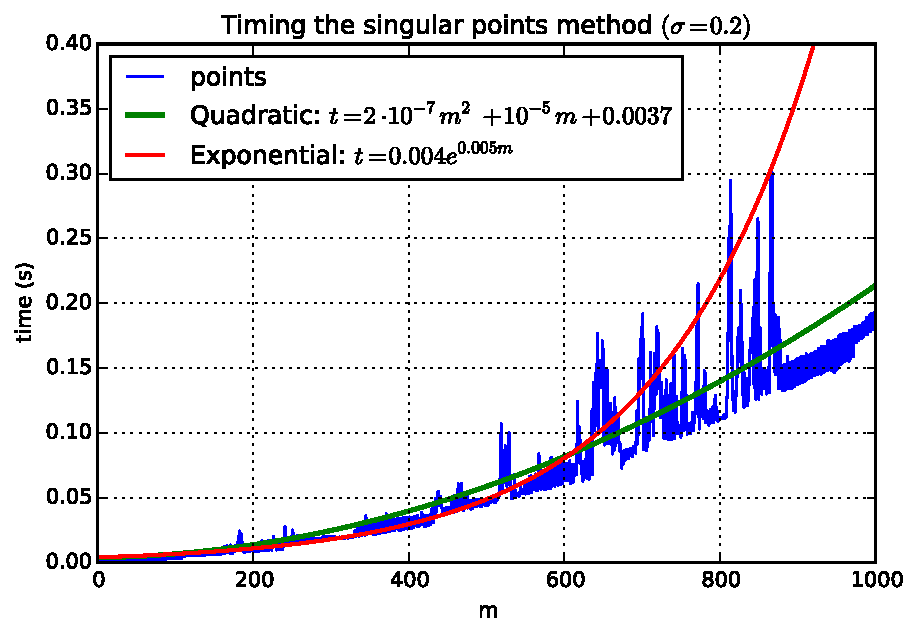
\includegraphics[width=\linewidth]{img/timing-cliquet}
	\caption[Timing -- cliquet]{Timing the singular point method for cliquet option with constant volatility $ \sigma = 0.2 $. The quadratic curve provides a pragmatic bound for the runtimes. The exponential curve is too conservative.}
	\label{fig:clq-timing}
\end{figure}


\begin{rem}[Computational complexity]
	We remarked earlier that although the computational complexity of the algorithm without approximation is the same as that of the binomial model, enabling approximations decreases the complexity to a polynomial time algorithm. In fact, the Figure \ref{fig:clq-timing} corroborates exactly to this. The blue dots denotes the time taken to run the algorithm for constant volatility of $ \sigma = 0.2 $. The green line is a quadratic function of the number of time steps $ m $, whereas the red line is an exponential function of the same. We varied the parameters so that the curves fits the data. We see that the quadratic function serves as an upper bound for the running time for most data points in the plot, except for a few points, which may be treated as outliers. Thus, we may conclude that the computational complexity of the algorithm is $ O(m^2) $ in this case. In fact, our experiments show that this is indeed the general trend. Thus, even though we have not found out the theoretical complexity of the algorithm, in practice the algorithm is competitive.
	
	Note that for the Asian case, the experimental complexity is $ O(n^3) $, whereas in the cliquet case, it is $ O(m^2) $.
\end{rem}


\paragraph{Concluding remarks}
We note that, in all cases, the difference between the prices in obtained by the singular points method and the binomial method is significantly smaller than the theoretical value of $ N \cdot 10^{-6} $. Moreover, as in the case examined $ N C_{loc} < C_{glob} $ (which is equivalent to $ N C_{loc} = C_{glob} $), the price functions $ V_i(Z) $ are always convex and this implies that the approximation procedure will provide an upper estimate of the exact binomial value.

Thus, the singular points method is quite capable in pricing cliquet options in a Black-Scholes framework with piecewise constant interest rates and volatilities. The implementation is quite simple, and the price obtained by the method converges to the price of continuous model. In absence of approximation, the price matches the exact binomial price. The ability to set \emph{a priori} error bounds differentiates it from the alternative algorithms.

Numerical comparisons indicate that the method is accurate both for standard and small volatilities, and that it avoids the computational problems arising from the application of the standard binomial method. For small volatilities and large numbers of observation times in particular, the improvement with respect to the binomial standard technique is very significant. Experimental results show that the computational complexity in practice is around $ O(m^2) $.


%%% Local Variables:
%%% LaTeX-command: "latex -shell-escape"
%%% mode: latex
%%% TeX-master: t
%%% End:


\chapter{Epilogue}
\label{cha:epilogue}
% !TeX root = ../thesis.tex
% !TeX spellcheck = en_GB
% !TeX encoding = UTF-8


In the thesis, our main focus was to develop the ideas behind the pricing of options, and to study two particular classes of path-dependent exotic options, namely Asian options and cliquet options. We saw that these options do not lend themselves to be priced under the Black-Scholes framework, and we have to resort to alternative ways of pricing them. They can be priced in the Cox-Ross-Rubinstein model, but the complexity is exponential with respect to the number of time steps, and is infeasible in practice. The singular points method is a new lattice based method which has the same theoretical complexity as the Cox-Ross-Rubinstein model. But it excels in allowing for approximations, and this reduces the complexity from exponential time to polynomial time of very low orders.

Albeit similar in the basic structure, the theory of how the singular points method may be applied for Asian options and cliquet options are quite different, as are the corresponding algorithms. On the one hand, in the case of Asian options, we saw that the algorithm neither did generalise for Asian options with geometric mean, nor for local volatility models. Moreover, the pre-existing algorithms (some lattice-based) were quite competitive to this method.

On the other hand, for cliquet options, the method was able to handle cases of variable rates of interest, volatility, and local caps and floors with ease. The algorithm is extremely fast in this case, and does in fact outdo most other competing algorithms in terms of simplicity, ease of implementation and low memory requirement. Furthermore, this seems to be one of the very few tree lattice-based methods available to price cliquet options.

As a further research, it might be interesting to explore on the possibility of customising the method for other exotic option types. It would also be interesting to conduct a further study on the theoretical complexity of the algorithm, especially the dependence of the number, closeness and removability of singular point with respect to initial data ($ S_0, K, T, \sigma, r, F_{loc}, C_{loc}, F_{glob}, C_{glob} $) and the computational parameters ($ m, h $).

In conclusion, the method is quite specific; its implementation depends very much on the type of option. Nevertheless, it is a significant leap in the domain of tree methods because of its inherent advantages over other methods.


%%% Local Variables:
%%% mode: latex
%%% TeX-master: t
%%% End:



\appendix
\chapter{Probability Theory}
\label{cha:probability}
% !TeX root = ../thesis.tex
% !TeX spellcheck = en_GB
% !TeX encoding = UTF-8


\section{Probability review}

Probability spaces

Measurability

Random variable

Stochastic process

Conditional expectation

Filtrations

Adaptation

Martingale

Absolutely continuous measure, Radon-Nikodym derivative

measurable functions may be treated as constant under conditional expectation

Characteristic function

Convergence in distribution

Brownian motion

Stochastic calculus and Ito's Lemma

%%% Local Variables:
%%% mode: latex
%%% TeX-master: t
%%% End:



\backmatter

\listoffigures

%\listofalgorithms

\printbibliography


\end{document}



%%% Local Variables:
%%% mode: latex
%%% TeX-master: t
%%% End:
